\documentclass[12pt, a4paper, twoside]{report}
\usepackage{amsmath, amssymb}
\usepackage{geometry}
\usepackage{fancyhdr}
\usepackage{graphicx}
\usepackage{titlesec}
\usepackage{fontspec}
\usepackage{tocloft} 
\usepackage{natbib}
\usepackage{float}
\usepackage{colortbl}
\usepackage{enumitem}
\usepackage[table]{xcolor}

\graphicspath{ {./images/} }

% Page settings
\geometry{
    a4paper,
    top=5cm,
    bottom=4.8cm,
    left=3.7cm,
    right=3.7cm,
    headheight=4.3cm, % Header height set to 4.3 cm
     headsep=0.5cm, % Adjust this value if needed to control spacing between header and text
    footskip=0cm % No extra space for footer
}


\definecolor{lightgreen}{rgb}{0.82, 0.94, 0.75}
\definecolor{lightorange}{rgb}{0.98, 0.84, 0.65}
\newcolumntype{L}{>{\centering\arraybackslash}m{10cm}}
\newcolumntype{l}{>{\centering\arraybackslash}m{7cm}}
\def\BibTeX{{\rm B\kern-.05em{\sc i\kern-.025em b}\kern-.08em
    T\kern-.1667em\lower.7ex\hbox{E}\kern-.125emX}}

\setlist[itemize]{itemsep=0pt, topsep=0pt, parsep=0pt, partopsep=0pt}

% Font settings
\setmainfont{Verdana}
\newfontface\symbolsfont{Symbol} % For unsupported mathematical symbols

% Title and section fonts with sizes
\titleformat{\chapter}[hang]{\fontsize{14pt}{14pt}\selectfont\bfseries}{\thechapter.}{20pt}{\fontsize{14pt}{14pt}\selectfont\bfseries}
\titleformat{\section}[hang]{\fontsize{11pt}{11pt}\selectfont\bfseries}{\thesection.}{12pt}{\fontsize{11pt}{11pt}\selectfont\bfseries}
\titleformat{\subsection}[hang]{\fontsize{10pt}{10pt}\selectfont\bfseries}{\thesubsection.}{10pt}{\fontsize{10pt}{10pt}\selectfont\bfseries}


% Paragraph indent and spacing
\setlength{\parindent}{1.27cm} % Tabs equivalent to 1.27 cm
\setlength{\parskip}{9pt} % Spacing between paragraphs
% Fancy header settings

\pagestyle{fancy}
\fancyhf{} % Clear all header and footer fields

% Header settings

\fancyhead[RO]{\fontsize{9pt}{11pt}\selectfont  \thechapter \hspace{0.1em} - \hspace{0.1em} \rightmark \hspace{1em} \thepage}  % Odd pages: Section title on the right, then page number
\fancyhead[LE]{\fontsize{9pt}{11pt}\selectfont \thepage \hspace{1em} \leftmark \hspace{0.1em} - \hspace{0.1em} \thechapter}  % \thesection Even pages: Page number on the left, then chapter title

\renewcommand{\chaptermark}[1]{\markboth{#1}{}} % Only chapter title in the header
\renewcommand{\sectionmark}[1]{\markright{#1}}

\fancypagestyle{plain}{
    \fancyhf{} % Clear all header and footer fields for chapter start pages
    \renewcommand{\headrulewidth}{0pt} % Remove header line
    \renewcommand{\footrulewidth}{0pt} % Remove footer line
}

% TOC, List of Figures, and List of Tables Customizations

% Suppress the default ToC, LoF, LoT titles by making them empty
\renewcommand{\contentsname}{}
\renewcommand{\listfigurename}{}
\renewcommand{\listtablename}{}

% Manually insert a centered, bold, uppercase title in the respective pages
\addtocontents{toc}{\protect\begin{center}\MakeUppercase{\bfseries\fontsize{9pt}{14pt}\selectfont Contents}\protect\end{center}\vspace*{-1em}\vspace{1\baselineskip}}
\addtocontents{lof}{\protect\begin{center}\MakeUppercase{\bfseries\fontsize{9pt}{14pt}\selectfont List of Figures}\protect\end{center}\vspace*{-1em}\vspace{1\baselineskip}}
\addtocontents{lot}{\protect\begin{center}\MakeUppercase{\bfseries\fontsize{9pt}{14pt}\selectfont List of Tables}\protect\end{center}\vspace*{-1em}\vspace{1\baselineskip}}

% Ensure entries in the Table of Contents, List of Figures, and List of Tables are in normal font
\renewcommand{\cftchapfont}{\normalfont\fontsize{9pt}{11pt}\selectfont} % Chapter entries in normal font
\renewcommand{\cftsecfont}{\normalfont\fontsize{9pt}{11pt}\selectfont} % Section entries in normal font
\renewcommand{\cftsubsecfont}{\normalfont\fontsize{9pt}{11pt}\selectfont} % Subsection entries in normal font
\renewcommand{\cftchappagefont}{\normalfont\fontsize{9pt}{11pt}\selectfont} % Page numbers for chapters in normal font
\renewcommand{\cftsecpagefont}{\normalfont\fontsize{9pt}{11pt}\selectfont} % Page numbers for sections in normal font
\renewcommand{\cftsubsecpagefont}{\normalfont\fontsize{9pt}{11pt}\selectfont} % Page numbers for subsections in normal font
\renewcommand{\cftdotsep}{1} % Set dot separation for entries to be closer together


% Title and section fonts with sizes
\titleformat{\chapter}[block]
  {\centering\normalfont\fontsize{14pt}{14pt}\selectfont\bfseries}
  {\thechapter.} 
  {0.5em} 
  {\MakeUppercase} 
  [\vspace{0pt}] 

% Spacing before and after chapters and sections to control vertical positioning
\titlespacing*{\chapter}{1.27cm}{3pt}{18pt} % 3 spaces of 9pt before chapter, 2 spaces of 9pt after chapter title
\titlespacing*{\section}{1.27cm}{18pt}{9pt} % 2 spaces of 9pt before section, 1 space of 9pt after section title
\titlespacing*{\subsection}{1.27cm}{9pt}{9pt} % 1 space of 9pt before and after subsection


% Adjust Table of Contents Layout


\setlength{\cftchapindent}{0pt} % No indent for chapters
\setlength{\cftsecindent}{1.5em} % Set indent for sections
\setlength{\cftsubsecindent}{3em} % Set indent for subsections
\setlength{\cftsubsubsecindent}{4.5em} 

\setlength{\cftchapnumwidth}{2em} % Set space for chapter numbers
\setlength{\cftsecnumwidth}{3em}  % Set space for section numbers
\setlength{\cftsubsecnumwidth}{4em} % Set space for subsection numbers

\let\origaddcontentsline\addcontentsline
\renewcommand{\addcontentsline}[3]{\origaddcontentsline{#1}{#2}{\numberline{}#3}}

\setlength{\cftbeforechapskip}{0pt}

\renewcommand{\normalsize}{\fontsize{9pt}{11pt}\selectfont}
\normalsize 

\def\BibTeX{{\rm B\kern-.05em{\sc i\kern-.025em b}\kern-.08em
    T\kern-.1667em\lower.7ex\hbox{E}\kern-.125emX}}

\newcommand*{\Comb}[2]{{}^{#1}C_{#2}}%

\begin{document}
\vspace*{-4cm}
\pagestyle{empty}
\tableofcontents
\clearpage

\newpage
\vspace*{-4cm}
\listoftables

\newpage
\vspace*{-4cm}
\listoffigures


\pagestyle{fancy}


\newpage

\chapter{Introduction}
\section{Research scope and motivation}


The domain of the proposed thesis is Automated Software Engineering. The thesis will develop methods for the analysis of legacy software systems, focusing on using historical information describing the evolution of the systems extracted from the versioning systems. 
The methods for analysis will integrate techniques based on computational algorithms as well as data-mining. As proof-of-concept, tool prototypes will implement the proposed methods and validate them by extensive experimentation on several cases of real-life systems.\\

\section{Objectives of the thesis}



\section{Structure of the thesis}

\section{Main Contributions}



%%%%%%%%%%%%%%%%%%%%%%%%%%%%%%%%%%%%%%%%%%%%%%%%%%%%%

\chapter{Software Dependencies: concepts, applications, and current research}
\label{dep}

\section{Software dependencies overview}

\subsection{Structural dependencies}
\hspace{4em} A dependency is created by two elements that are in a relationship and indicates that an element of the relationship, in some manner, depends on the other element of the relationship \cite{Booch:2004:OAD:975416}, \cite{Cataldo2009SoftwareDW}.

Structural dependencies can be found by analyzing the source code \cite{Sangal:2005:UDM:1094811.1094824}, \cite{CalloArias2011}. 
There are several types of relationships between these source code entities and all those create \textit{structural dependencies}:

\textbf{Data Item Dependencies.}
Data items can be variables, records or structures. A dependency is created between two data items when the value held in the first data item is used or affects the value from the second.


\begin{verbatim}
Example:

int a = 10;
int b = a + 5;  // b depends on a
a = 20;         // changing a doesn't impact b
\end{verbatim}

\textbf{Data Type Dependencies.}
Data items are declared to be of a specific data type. Besides the built-in data types that every programming language has, developers can also create new types that they can use. Each time the data type definition is changed it will affect all the data items that are declared to be of that type. 


\begin{verbatim}
Example:

class Rectangle { int width, height; }
//Change posibility: class Rectangle { int width, height, color; }

Rectangle r = new Rectangle();  
r.width = 5;
r.height = 10;
// Existing code will fail to handle color in case of change
\end{verbatim}

\textbf{Subprogram Dependencies.}
A subprogram is a sequence of instructions that performs a certain task. Depending on the programming language a subprogram may also be called a routine, a method, a function or a procedure. When a subprogram is changed, the developer must check the effects of that change in all the places that are calling that subprogram. Subprograms may also have dependencies with the data items that they receive as input or the data items that they are computing.


\begin{verbatim}
Example:

// First implementation:
class Calculator {
    double calculateArea(double side) {
        return side * side;  
    }
}

// Modified implementation:
class Calculator {
    double calculateArea(double radius) {
        return Math.PI * radius * radius; 
    }
}

Calculator calc = new Calculator();
// Code expecting square area now gets circle area.
double area = calc.calculateArea(5);  

\end{verbatim}





\subsection{Lexical dependencies}

\hspace{4em}Lexical dependencies, similar to structural dependencies, are extracted from the source code. The difference lies in the fact that lexical dependencies focus on finding pairs of entities that are similar (and thus connected) from a linguistic point of view. This means they are based on the textual content and naming conventions used in the code rather than explicit structural relationships. The lexical information about an entity (such as a class or interface) can be extracted from class names, method names, parameter names, code comments, source code statements, and others \cite{lexical-dep}, \cite{lexical-dep-Prajapati}.

For example, a class named \texttt{StructuralDependenciesEvaluator} and a class named \texttt{LexicalDependenciesEvaluation} can be related even if they do not directly share dependencies or their connection is not visible from a structural point of view.

To extract lexical dependencies, the code is tokenized, breaking it down into lexical tokens (e.g., words or symbols). A document containing these tokens is created for each source code file. Each document is then split into different parts, such as a class names part, attribute names part, parameter names part, and others. For instance, the class names part will contain the names of all classes found in the source file.

After the tokenization process and splitting into various parts, the similarity between the two documents is estimated. 

Various methods can be used for similarity calculation, such as:
\begin{itemize}
    \item \textit{Term Frequency-Inverse Document Frequency (TF-IDF):} Weighs the importance of words based on their frequency across documents \cite{lexical-dep}, \cite{lexical-dep-Corazza}.
    \item \textit{Cosine Similarity:} Measures the cosine of the angle between two vectors representing the documents \cite{lexical-dep-Prajapati}.
\end{itemize}






\subsection{Semantical dependencies}

\hspace{4em} Podgurski and Clarke define semantic dependencies in source code as follows: if changes in a statement \(s_1\) impact the behavior of another statement \(s_2\), then \(s_1\) and \(s_2\) are \emph{semantically dependent} \cite{Podgurski-semantic}.

Semantic dependencies can be identified from the source code by constructing control flow graphs (CFGs). A control flow graph is a directed graph \(G = (V, E)\), where:
\begin{itemize}
    \item \(V\) is the set of vertices representing program statements (e.g., assignments, method calls, conditions),
    \item \(E\) is the set of edges representing possible transfers of control between statements.
\end{itemize}

A vertex \(u \in V\) is semantically dependent on a vertex \(v \in V\) if changes in \(v\) determine changes in \(u\).

In object-oriented (OO) systems, semantic dependencies are dependencies that are not visible in the static structure of the code. There is no direct reference between two entities (e.g., classes or interfaces), but changes in one entity impact the behavior of the other \cite{Neto-semantic-dep}, \cite{Capiluppi-semantic-dep}.


\textit{Example:}

Let \(A\) a class that uses an object of type \(I\), and let \(B\) a class that implements \(I\). For example, class \(A\) calls a method \texttt{performAction()} via an interface \(I\), while class \(B\) implements the \texttt{performAction()} method.

If \(B\) changes its implementation of \texttt{performAction()}, the behavior of \(A\) might also change when it uses \(B\). This means that \(A\) and \(B\) are semantically dependent.






\subsection{Logical dedependencies}
\hspace{4em} \textit{Logical dependencies} (also known as logical coupling) can be discovered through software history analysis. They reveal relationships between entities that are not always present in the source code's static structure (i.e., structural dependencies).

Software engineering practice has shown that sometimes modules without explicit structural dependencies still appear to be related. \textit{Co-evolution} represents the phenomenon where one component changes in response to changes in another component \cite{Yu:2007:UCC:1231330.1231370, 5166450}. Such changes can be found in the software history maintained by version control systems. Gall et al. defined \textit{logical coupling} as the occurrence of modules that \emph{repeatedly} update together during the evolution of the software system \cite{Gall:1998:DLC:850947.853338, Gall:2003:CRH:942803.943741, 6606615}.

The concepts of logical coupling and logical dependencies have been applied in different analysis tasks related to software changes: for software change impact analysis \cite{1553643}; for identifying potential ripple effects caused by software changes during maintenance and evolution \cite{DBLP:conf/issre/OlivaG15, Oliva:2011:ISL:2067853.2068086, Poshyvanyk2009, posh2010}; and for exploring their link to defects \cite{wiese, Zimmermann:2004:MVH:998675.999460}.

An in-depth analysis of how logical dependencies are identified within the versioning system and their applications is provided in Section \ref{ld-intro}.






\subsection{Additional dependencies}

\hspace{4em} Besides the dependencies mentioned above, there are many other types of dependencies, such as temporal, package, external, and several others.

\textit{Temporal dependencies} represent a type of dependency where certain operations in the code must occur in a specific order. These operations may belong to the same software component or span across different parts of the system \cite{work-dep}.

\begin{verbatim}
Example:

var file = new File();
file.open("example.txt");
file.readContents();
file.close();
\end{verbatim}

In this example, there is a temporal dependency between the \texttt{open}, \texttt{readContents}, and \texttt{close} methods. The \texttt{readContents} method cannot function correctly unless the \texttt{open} method is called first to open the file. Similarly, the \texttt{close} method should be called after \texttt{readContents} to release the file resources.


\textit{Package dependencies} refer to the relationships between different software packages, usually managed using package managers \cite{dep-package}.

\textit{External dependencies} are the relationships between a software system's code and components outside the system, such as third-party services, libraries, APIs, or the programming language itself \cite{dep-external}.






\section{Software change and version control systems}

\subsection{Software change}
\label{change}

\hspace{4em} Software systems have distinctive stages during their life: initial development, evolution, servicing, phase out, and close down \cite{Software-life-cycle}, \cite{model-bennett}.

In the \textit{evolution stage}, iterative changes are made. By changes, we mean additions (new software features), modifications (changes of requirements or misunderstood requirements), or deletions. There are two main reasons for the change: the software team's learning process and new requests from the client.

Suppose new changes are no longer easy to be made or are very difficult and time-consuming. In that case, the software enters the \textit{servicing stage}, also called aging software, decayed software, and legacy \cite{Software-life-cycle}, \cite{363157}.

The main difference between changes made in the evolution and servicing stages is the effort to make changes. In the evolution stage, software changes are made easily and do not require much effort, while in the servicing stage, only a limited number of changes are made and require a lot of effort, so they are time-consuming \cite{Bennett}, \cite{Rajlich}.

The change mini-cycle consists of the following phases \cite{810308}:
\begin{itemize}
\item Phase 1: The change request. This usually comes from the software users, and it can also be a bug report or a request for additional functionality.
\item Phase 2: The planning phase includes program comprehension and change impact analysis. Program comprehension is a mandatory prerequisite of the change, while change
impact analysis indicates how costly the change will be. \cite{Bohner}
\item Phase 3: The change implementation, restructuring for change, and change propagation.
\item Phase 4: Verification and validation.
\item Phase 5: Re-documentation.
\end{itemize}

Understanding these phases is important for ensuring the software system remains maintainable and reliable throughout its lifecycle.


\subsection{Version control systems}

Software evolution implies change which can be triggered either by new feature requests or bug reports \cite{articleEvolution}. As presented also in section \ref{change}, one phase of the change mini-cycle consists of change implementation and propagation (changing source code files). 
Usually, developers use version control when it comes to software development. Version control is a system that records changes to a file or set of files over time so that developers can recall specific versions of those files later \cite{svn}.
Distributed version control systems (such as Git, Mercurial, Bazaar or Darcs) allows many developers to collaboratively develop their projects \cite{7471284}.

Below, we will review some of the operations supported by versioning systems. The operation names in the following text are specific to Git, as Git is the version control system used for data collection in the current work. However, similar operations exist in other versioning systems; for example, Subversion (SVN) and Mercurial also provide operations such as branching, merging, and committing changes.

\textbf{Repository}

A repository serves as a centralized storage location for project files. The entire codebase of a project can be stored within a single repository or be split into a main repository and various modules stored in multiple repositories. Git repositories can be hosted on numerous platforms, such as GitHub, GitLab, Bitbucket, and others.

It is important to differentiate between Git and Git hosting services. Git is a version control system that allows developers to download and modify code on their local devices while hosting services like GitHub provide platforms for teams to host projects that utilize Git \cite{git}, \cite{github}.

\textbf{Commits}

Committing is an operation that allows developers to record the latest changes to the codebase in the repository. A commit saves the current state of the code, including changes made since the last commit.

The changes tracked include:

\begin{itemize}
\item \textit{Additions:} New files or lines of code created.
\item \textit{Modifications:} Updates to existing lines of code or files.
\item \textit{Deletions:} Removal of files or lines of code that are no longer needed.
\end{itemize}

The \textit{push} operation uploads these changes to the remote repository on the hosting service.

A unique identifier, also known as a commit hash, is assigned to each commit. This hash allows developers to track specific changes or revert to earlier code versions. When a developer commits the changes, a commit message is required. This message serves as documentation for the changes, enhancing code traceability and maintainability \cite{git}.

Figure~\ref{fig:gitflow} illustrates how changes are made to the code over time through commits, starting from the initial commit to the latest version.

\begin{figure}[h!]
\centering
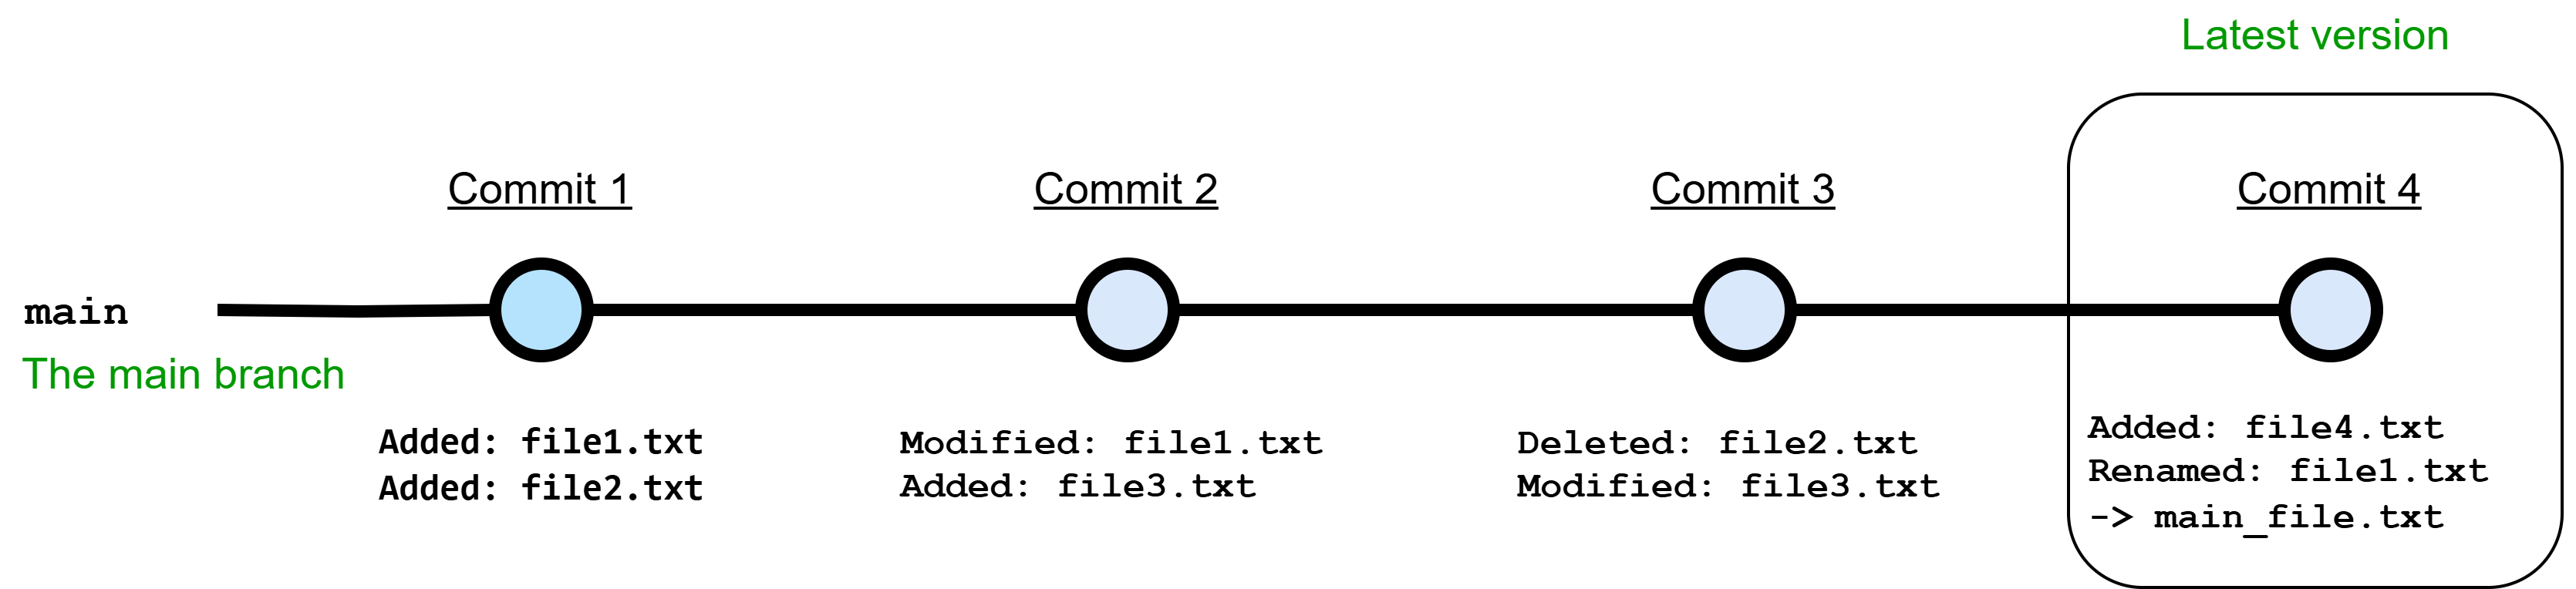
\includegraphics[width=\textwidth]{gitflow.png}
\caption{Tracking changes through commits.}
\label{fig:gitflow}
\end{figure}

\textbf{Branches and Merging}

By default, every repository comes with a main (or master) branch. This branch represents the central timeline for code changes and serves as the main integration point for stable code. Other branches can be created for parallel development from this branch.

Branches allow developers to encapsulate changes without affecting the main branch. In most software projects, it is standard practice for developers to use branches for development, with the main branch being locked for direct commits. Changes to the main branch can be integrated through merges from other branches.

Software projects often have multiple branches running in parallel, including branches from other branches. The main branch is not the only branch that supports branching; any branch can be a base for creating other branches.

The operation of integrating changes from one branch into another (usually into the main branch) is called \textit{merging}.

There are three main types of merges in Git \cite{git}:

\begin{itemize}
    \item \textit{Git Merge:} This is the most commonly used type of merging. It creates a new merge commit that combines all the changes from the branch being merged. Additionally, it retains the history of all the individual commits in the branch.
    \begin{verbatim}
    git checkout main
    git merge feature-branch
    \end{verbatim}

    \item \textit{Git Rebase and Merge:} This operation is typically used when the branch contains a single commit or a small number of commits. It moves all the commits from the source branch to the top of the target branch. The main disadvantage of this operation is that it rewrites the commit history.
    \begin{verbatim}
    git checkout feature-branch
    git rebase main
    git checkout main
    git merge feature-branch
    \end{verbatim}

    \item \textit{Git Squash and Merge:} This operation compresses all commits from the source branch into a single commit before merging it into the target branch. It results in a cleaner commit history but has the disadvantage of losing individual commits from the source branch.
    \begin{verbatim}
    git checkout main
    git merge --squash feature-branch
    git commit
    \end{verbatim}
\end{itemize}


Figure~\ref{fig:merging} illustrates the differences between these three types of merging. 

\begin{figure}[h!]
    \centering
    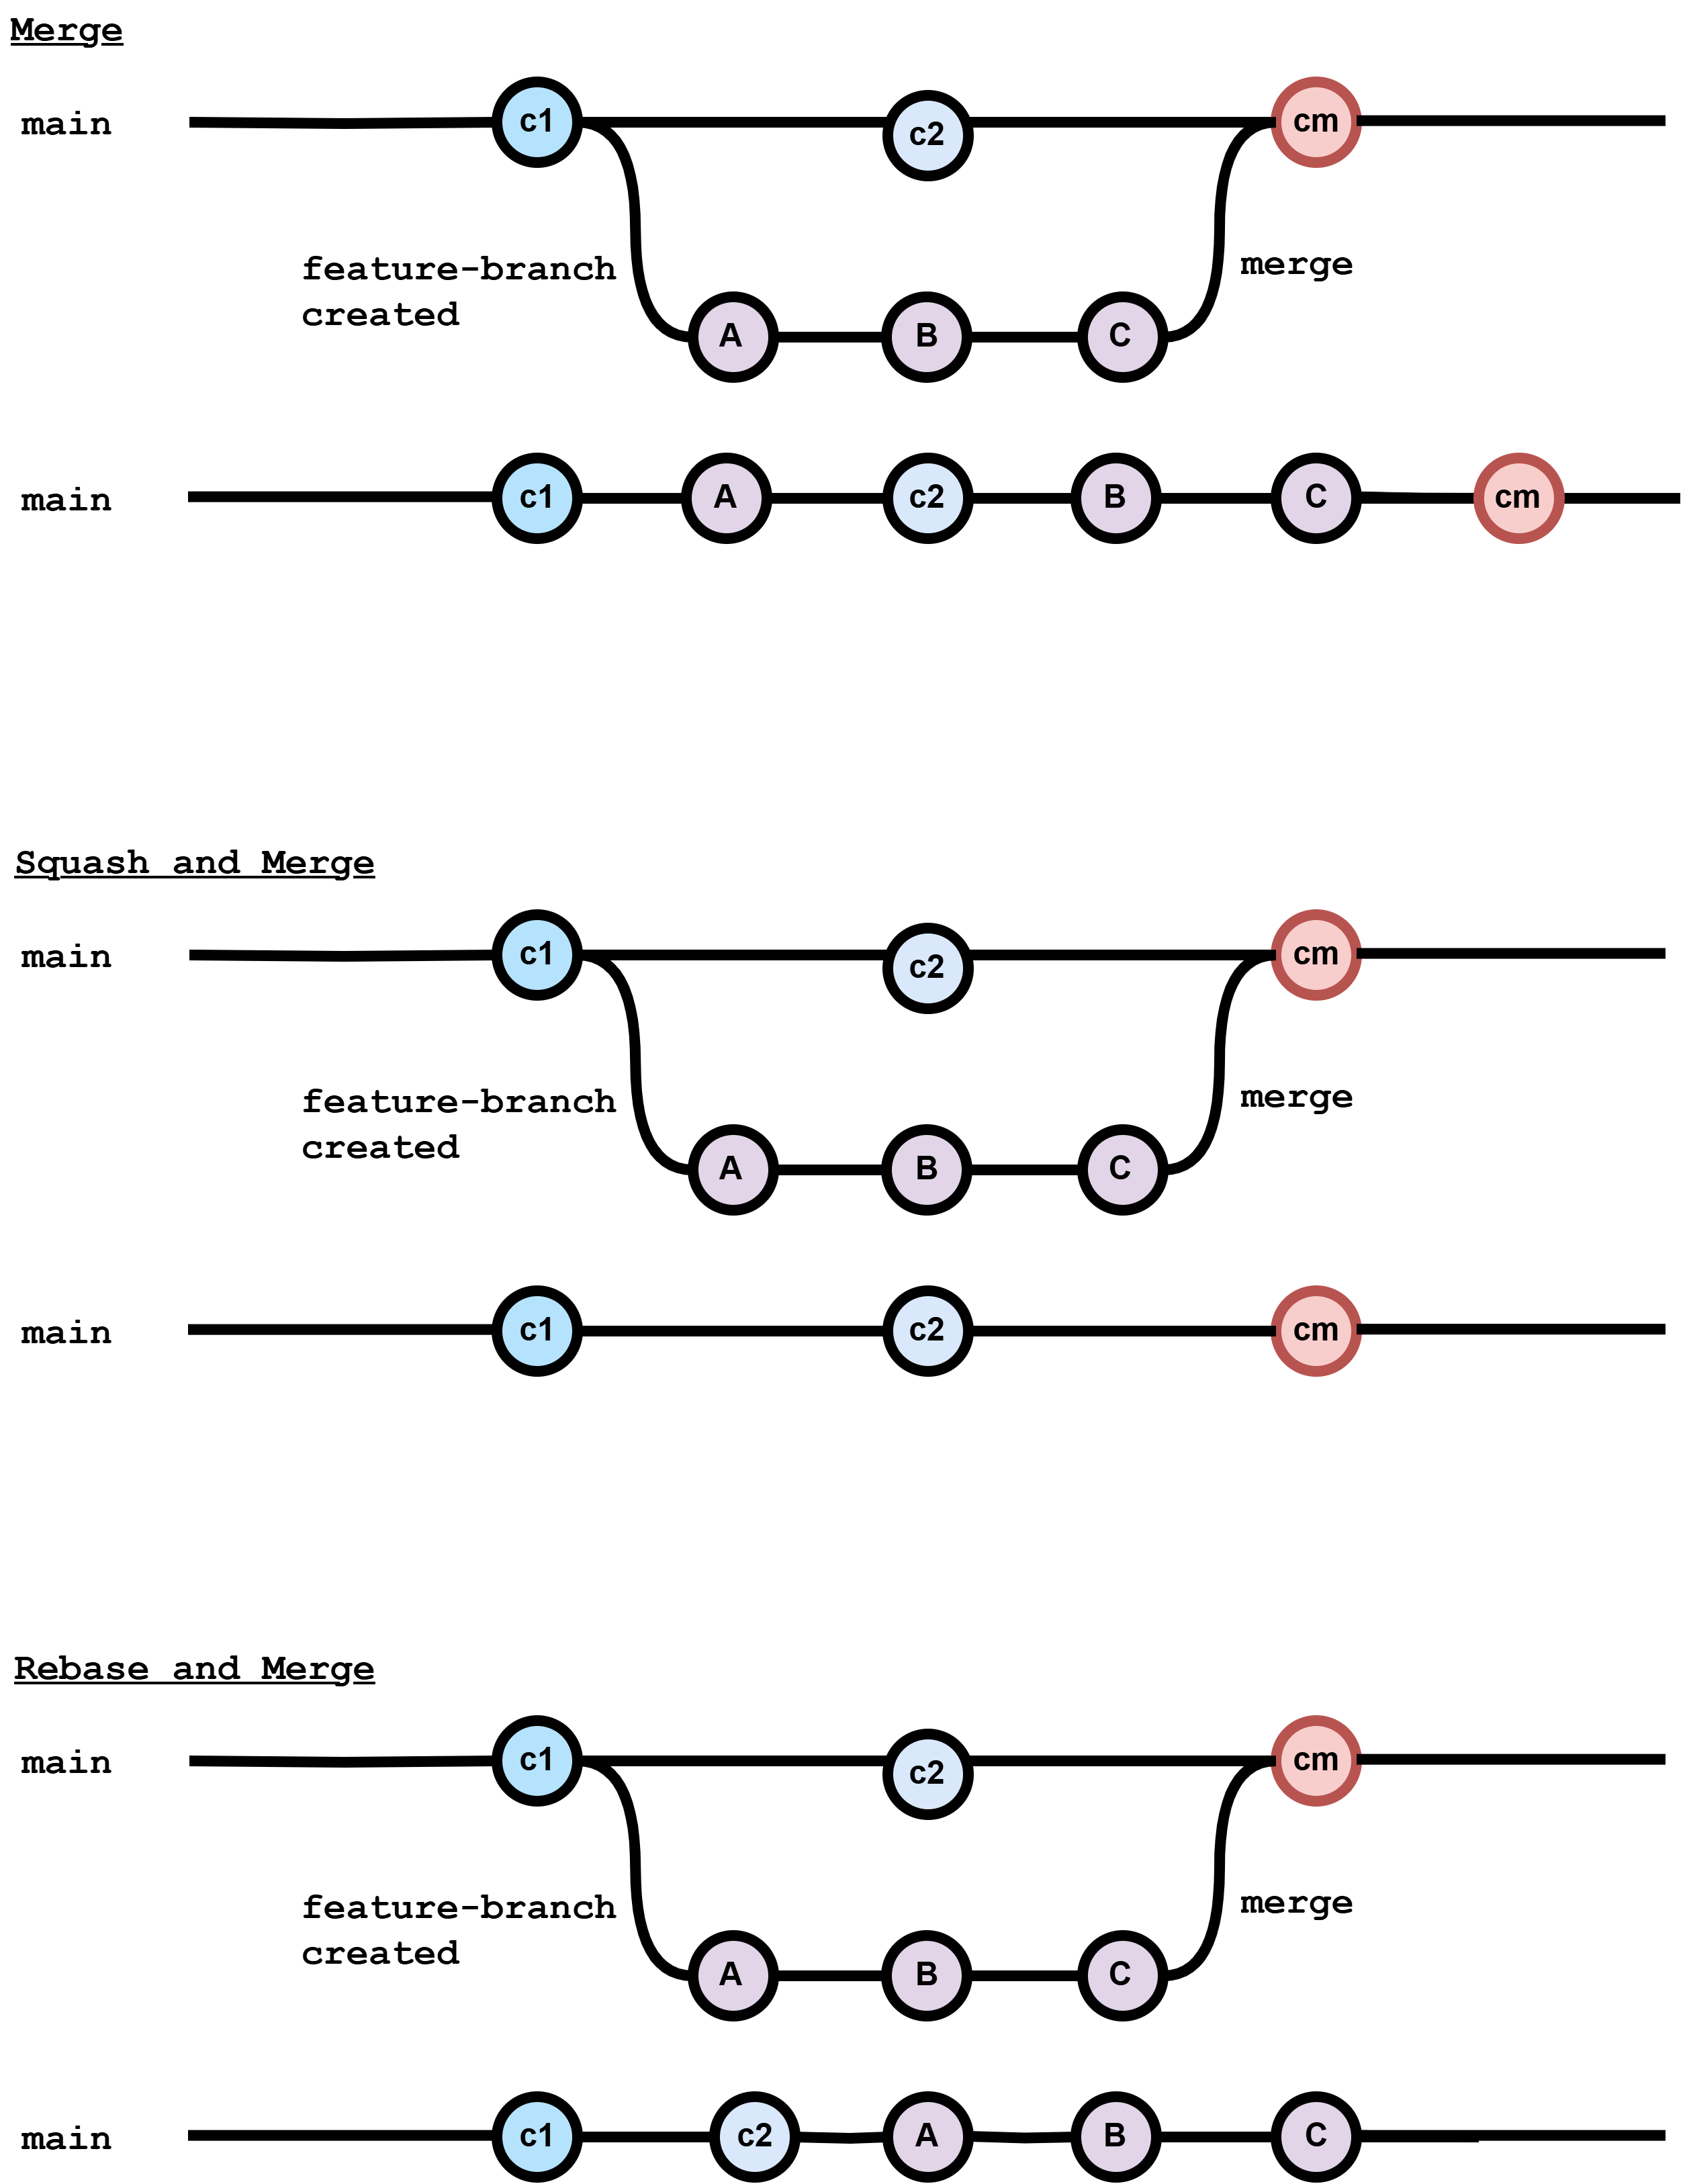
\includegraphics[width=\textwidth]{merging.png}
    \caption{Comparison of Git merge types.}
    \label{fig:merging}
\end{figure}

\textbf{Tagging}

Another helpful operation in Git is tagging. Developers use the tagging operation to mark a specific code version at a particular commit. This is usually done for important milestones, such as a new release version or a stable build \cite{git}.

Tags provide a way to create a human-readable reference to a specific commit (e.g., \texttt{v1.0.0}), as the commit hash can be hard to remember (e.g., \texttt{a1b2c3d4e5f6g7h8i9})

Git supports two types of tags:
\begin{itemize}
    \item \textit{Lightweight Tags:} Simple references to a commit that do not contain any additional metadata.
    \item \textit{Annotated Tags:} These include additional metadata such as the author's name, date, and message, making them more suited for marking releases.
\end{itemize}



\section{Current status of research on logical dependencies}
\label{ld-intro}

\subsection{Logical dependencies in software systems}

Oliva and Gerosa \cite{Oliva:2011:ISL:2067853.2068086}, \cite{DBLP:conf/issre/OlivaG15} have found first that the set of co-changed classes was much larger compared to the set of structurally coupled classes. They identified structural and logical dependencies from 150000 revisions from the Apache Software Foundation SVN repository. Also they concluded  that in at least 91\% of the cases, logical dependencies involve files that are not structurally related. This implies that not all of the change dependencies are related to structural dependencies and there could be other reasons for software artifacts to be change dependent.

Ajienka and Capiluppi also studied the interplay between logical and structural coupling of software classes. In \cite{DBLP:journals/jss/AjienkaC17} they  perform experiments on 79 open source systems: for each system, they determine the sets of structural dependencies, the set of logical dependencies and the intersections of these sets. They quantify the overlapping or intersection of these sets, coming to the conclusion that not all co-changed class pairs (classes with logical dependencies) are also linked by structural dependencies. One other interesting aspect which has not been investigated by the authors in \cite{DBLP:journals/jss/AjienkaC17}  is the total number of logical dependencies, reported to the total number of structural dependencies of a software systems. However, they provide the raw data of their measurements and we calculated the ratio between the number of logical dependencies and the number of structural dependencies for all the projects analyzed by them: the average ratio resulted 12.  This means that, using their method of detecting logical dependencies for a system, the number of logical dependencies outnumbers by one order of magnitude the number of structural dependencies. We consider that such a big number of logical dependencies needs additional filtering. 


Another kind of non-structural dependencies are the semantic or conceptual dependencies \cite{Poshyvanyk2009}, \cite{posh2010}. Semantic coupling is given by the degree to which the identifiers and comments from different classes are similar to each other. Semantic coupling could be an indicator for logical dependencies, as studied by Ajienka et al in \cite{DBLP:journals/ese/AjienkaCC18}. The experiments showed that a large number of co-evolving classes do not present semantic coupling, adding to the earlier research which showed that a large number of co-evolving classes do not present structural coupling. All these experimental findings rise the question whether it is a legitimate approach to accept all co-evolving classes as logical coupling.

Zimmermann et al \cite{Zimmermann:2004:MVH:998675.999460} introduced data mining techniques to obtain association rules from version histories.
The mined association rules  have a probabilistic interpretation based on the amount of evidence in the transactions they are derived from. This amount of evidence is determined by two measures: support and confidence.  They developed a tool to predict future or missing changes.

Different applications based on dependency analysis could be improved if, beyond structural dependencies, they also take into account the hidden non-structural dependencies. For example, works  which investigate different methods for architectural reconstruction \cite{SoraConti}, \cite{SoraSem13}, \cite{PagerankENASE},  all of them based on the information provided by structural dependencies, could enrich their dependency models by taking into account also logical dependencies. However, a thorough survey \cite{sar} shows that historical information has been rarely used in architectural reconstruction. 

Another survey \cite{Shtern:2012:CMS:2332427.2332428} mentions one possible explanation why historical information have been rarely used in architectural reconstruction: the size of the extracted information. One problem is the size of the extraction process, which has to analyze many versions from the historical evolution of the system. Another problem is the big number of pairs of classes which record co-changes and how they relate to the number of pairs of classes with structural dependencies.

The software architecture is important in order to understand and maintain a system. Often code updates are made without checking or updating the architecture. This kind of updates cause the architecture to drift from the reality of the code over time \cite{sar}.
So reconstructing the architecture and verifying if still matches the reality is important \cite{Kalliamvakou2016}. 

Surveys also show that architectural reconstruction is mainly made based on structural dependencies \cite{Shtern:2012:CMS:2332427.2332428}, \cite{sar}, the main reason why historical information is rarely used in architectural reconstruction is the size of the extracted information.

Logical dependencies should integrate harmoniously with structural dependencies in an unitary dependency model: valid logical dependencies should not be omitted from the dependency model, but structural dependencies should not be engulfed by questionable logical dependencies generated by casual co-changes.  
Thus, in order to add logical dependencies besides structural dependencies in dependency models, class co-changes must be filtered until they remain only a reduced but relevant set of valid logical dependencies. 

Currently there is no set of rules or best practices that can be applied to the extracted class co-changes and can guarantee their filtering into a set of valid logical dependencies.
This is mainly because not all the updates made in the versioning system are code related. For example a commit that has as participants a big number of files can indicate that a merge with another branch or a folder renaming has been made. In this case, a series of irrelevant co-changing pairs of entities can be introduced. So, in order to exclude this kind of situations the information extracted from the versioning system has to be filtered first and then used.

Other works have tried to filter co-changes \cite{Oliva:2011:ISL:2067853.2068086}, \cite{DBLP:journals/jss/AjienkaC17}. One of the used co-changes filter is the commit size.The commit size is the number of code files changed in that particular commit. 
Ajienka and Capiluppi established a threshold of 10 for the maximum accepted size for a commit \cite{DBLP:journals/jss/AjienkaC17}. This means that all the commits that had more than 10 code files changed where discarded from the research. But setting a harcoded threshold for the commit size is debatable because in order to say that a commit is big or small you have to look first at the size of the system and at the trends from the versioning system. Even thought the best practices encourage small and often commits, the developers culture is the one that influences the most the trending size of commits from one system.

Filtering only after commit size is not enough, this type of filtering can indeed have an impact on the total number of extracted co-changes, but will only shrink the number of co-changes extracted without actually guaranteeing that the remaining ones have more relevancy and are more logical linked.

Although, some unrelated files can be updated by human error in small commits, for example: one file was forgot to be commited in the current commit and will be commited in the next one among some unrelated files. This kind of situation can introduce a set of co-changing pairs that are definitely not logical liked. In order to avoid this kind of situation a filter for the occurrence rate of co-changing pairs must be introduced. Co-changing pairs that occur multiple times are more prone to be logically dependent than the ones that occur only once. Currently there are no concrete examples of how the threshold for this type of filter can be calculated. In order to do that, incrementing the threshold by a certain step will be the start and then studying the impact on the remaining co-changing pairs for different systems. 

Taking into account also structural dependencies from all the revisions of the system was not made in previous works, this step is important in order to filter out the old, out-of-date logical dependencies. Some logical dependencies may have been also structural in previous revisions of the system but not in the current one. If we take into consideration also structural dependencies from previous revisions then the overlapping rate between logical and structural dependencies could probably increase. Another way to investigate this problem could be to study the trend of concurrences of co-changes: if co-changes between a pair of classes used to happen more often in the remote past than in the more recent past, it may be a sign that the problem causing the logical coupling has been removed in the mean time. 

\subsection{Existing filtering techniques}
tbd


\section{Applications of software dependencies}
\label{app}

\subsection{Reverse engineering}
The term reverse engineering was first defined by Chikofsky and Cross \cite{ChikofskyReverse} as the \textit{"process of analyzing a system to (i) identify the system’s components and
their inter-relationships and (ii) create representations of the system in another form or at a higher level of abstraction."} 

Reverse engineering is viewed as a two step process: information extraction and abstraction. \cite{FoSEReverseEngineering} 
The firs step, information extraction, is made by source code analysis which generates dependencies between software artifacts. So, reverse engineering uses dependencies in order to create new representations of the system or provide a higher level of abstraction \cite{struct_dep}, \cite{Gueheneuc}.

\subsection{Architecture reconstruction}
Currently, the software systems contain tens of thousands of lines of code and are updated multiple times a day by multiple developers.  
The software architecture is important in order to understand and maintain a system. Often code updates are made without checking or updating the architecture.
This kind of updates cause the architecture to drift from the reality of the code over time. So reconstructing the architecture and verifying if still matches the reality is important. \cite{sar},\cite{PagerankENASE}, \cite{Bass-archreconstruction} ,\cite{RecoverySartipi}, \cite{model-bennett}.

\subsection{Identifying clones}
Research suggests that a considerable part (around 5-10\%) of the source code of large-scale software is duplicate code (“clones”). Source code is often duplicated for a variety of reasons, programmers may simply be reusing a piece of code by copy and paste or they may be “reinventing the wheel” \cite{ClonesMayrand}, \cite{clones}.
Detection and removal of clones can decrease software maintenance costs \cite{CloneDetection}, \cite{cloneKamiya}.

\subsection{Code smells }
Code smells have been defined by Fowler \cite{bookFowler} and describe patterns that are generally associated with bad design and bad programming practices.
Originally, code smells are used to find the places in software may need refactoring \cite{articlesmells}. Studies have found that smells may affect comprehension and possibly increase change and fault proneness \cite{5741260}, \cite{5328703}, \cite{articlefault-proneness}.
Examples of code smells:
\begin{itemize}
	\item Large Class: one class with many fields.
	\item Feature Envy:  methods that access more methods and fields of another class than of its own class.
	\item Data Class: classes that only fields and do not contain functionality.
	\item Refused Bequest: classes that leave many of the fields and methods they inherit unused
	\item Parallel Inheritance: every time you make a subclass of one class you also have to make a subclass of the other.
	\item Shotgun Surgery: one method is changing together with other methods contained other classes.
\end{itemize}

Previous studies already explored the idea of using history information in order to detect code smells \cite{6963448}. 

\subsection{Comprehension}
Software comprehension is the process of gaining knowledge about a software system.
An increased knowledge of the software system help activities such as bug correction, enhancement, reuse and documentation \cite{Comprehension}, \cite{1199197}, \cite{2003:XLC:851042.857028}.
Previous studies show that the proportion of resources and time allocated to maintenance may vary from 50\% to 75\% \cite{articleLientz}.
Regarding maintenance, the greatest part of the software maintenance process is the activity of understanding the
system. 
Thanking into consideration the previous statements we can say that if we want to improve software maintenance we have to improve software comprehension \cite{article-cognitive-processes}.

\subsection{Fault location}
Debugging software is an expensive and mostly manual process. Of all debugging activities, fault localization, is the most expensive \cite{articleDebugging}. 

Software developers locate faults in their programs using a manual process. This process begins when the developers observe failures in the program. The developers choose a set of data to inject in the system(a set of data that most likely replicate previous failures or may generate new ones) and place breakpoints using a debugger. Then they observe the system's state until an failed state is reached, and then backtrack until the fault is found. 

As we said, this process has high costs so because of this high cost, any improvement in the process can decrease the cost of debugging.\cite{fault-localization} \cite{program-failures}


\subsection{Error proneness}
Research has shown that based on the software error history and simple metrics related to the amount of data and the structural complexity of software,
modules that are most likely to contain errors can be identified \cite{67595}, \cite{1702015}.


\subsection{Empirical software engineering research}
Empirical research tries to explore, describe, predict, and explain natural or social phenomena by using evidence based on observation or experience.
It involves obtaining and interpreting evidence by experimentation, systematic observation, interviews, surveys, or by the careful examination of documents and artifacts. \cite{inproceedingsEmpirical}

\chapter{Methodology for extracting and filtering logical dependencies}
\label{extraction}

\section{Overview of the approach}
\label{sec:overview_approach}

\hspace{4em}This chapter investigates the process of extracting and refining logical dependencies. The process is organized into three steps: collecting data, extracting dependencies, and applying filters.

A set of 27 open-source projects were used to perform the investigations. These projects have different sizes, complexities, and programming languages (Java and C\#). Section \ref{subsec:data_sets_used} provides an overview of the systems used.

The extraction process targets two types of dependencies:\\
- \textit{Structural dependencies} are obtained by analyzing the static structure of the source code. Using the \textit{srcML} tool, source code files are converted into an XML format to extract relationships between entities. \\
- \textit{Logical dependencies} are derived from the version control history. \\

After extraction, filtering techniques are applied to refine the logical dependencies:\\
- \textit{Commit size filtering} removes co-changing pairs from large commits, such as branch merges or formatting updates.\\
- \textit{Support filtering} ensures co-changing pairs occur a minimum number of times.\\
- \textit{Strength filtering} uses metrics like support, confidence, and a system factor to identify pairs with stronger relationships, scaling the results to the reality of the system.
- \textit{Code comments filtering} excludes co-changing pairs that involve only changes to code comments, as these are non-functional modifications.  

Each filtering step helps reduce the number of co-changing pairs while keeping meaningful dependencies. Figure \ref{fig:figworkflow} shows the workflow of the tool, which handles data collection, dependency extraction, and filtering. 



\section{Data collection}
\label{sec:data_collection}


\subsection{Data set used}
\label{subsec:data_sets_used}

\hspace{4em}To investigate logical dependencies extraction and filtering techniques and their interplay with structural dependencies, 27 open-source projects from GitHub\footnote{http://github.com/} were selected. Table \ref{table:1} provides an overview of all the software systems analyzed. The columns in the table represent the following information:

\hspace{-4em}- \textit{ID}: A unique identifier assigned to each project. \\
- \textit{Project name}: The name of the project as it appears on GitHub. \\
- \textit{Number of entities}: The total number of entities (classes and interfaces) extracted from the source code. \\
- \textit{Number of commits}: The total number of commits analyzed from the active branch (main/master) of each project. \\
- \textit{Type}: The programming language used in the development of the project.


This selection includes projects implemented in two programming languages: Java and C\#. The systems vary in size and complexity. From a structural perspective, the smallest project is \textit{shipkit}, which contains only 639 entities, while the largest is \textit{EntityFrameworkCore}, with 50,179 entities.

Regarding commit history, \textit{shipkit} is again the smallest, with 1,563 commits analyzed, while \textit{aeron} is the largest, with 5,977 commits. This selection of projects allows a better investigation of how filtering techniques affect systems of different sizes and commit histories.


\begin{table}[!h]
\renewcommand{\arraystretch}{1}
\caption{Summary of open source projects used for logical dependencies extraction and filtering.}
\label{table:1}
\centering
\scalebox{0.9}{
\begin{tabular}{|c|c|c|c|c|c|}
\hline
   ID  & Project name   & Number of & Number of& Type\\
     &     & entites & commits & \\
\hline
1	&	bluecove	&	2685	&	894	&	Java	\\
2	&	aima-java	&	5232	&	1006	&	Java	\\
3	&	powermock	&	2801	&	949	&	Java	\\
4	&	restfb	&	3350	&	1391	&	Java	\\
5	&	rxjava	&	21097	&	4398	&	Java	\\
6	&	metro-jax-ws	&	6482	&	2927	&	Java	\\
7	&	mockito	&	5189	&	3330	&	Java	\\
8	&	grizzly	&	10687	&	3113	&	Java	\\
9	&	shipkit	&	639	&	1563	&	Java	\\
10	&	OpenClinica	&	9655	&	3276	&	Java	\\
11	&	robolectric	&	8922	&	5912	&	Java	\\
12	&	aeron	&	4159	&	5977	&	Java	\\
13	&	antlr4	&	4747	&	4431	&	Java	\\
14	&	mcidasv	&	3272	&	4136	&	Java	\\
15	&	ShareX	&	4289	&	5485	&	C\#	\\
16	&	aspnetboilerplate	&	9712	&	4323	&	C\#	\\
17	&	orleans	&	16963	&	3995	&	C\#	\\
18	&	cli	&	2063	&	4488	&	C\#	\\
19	&	cake	&	12260	&	2518	&	C\#	\\
20	&	Avalonia	&	16732	&	5264	&	C\#	\\
21	&	EntityFrameworkCore	&	50179	&	5210	&	C\#	\\
22	&	jellyfin	&	8764	&	5433	&	C\#	\\
23	&	PowerShell	&	2405	&	3250	&	C\#	\\
24	&	WeiXinMPSDK	&	7075	&	5729	&	C\#	\\
25	&	ArchiSteamFarm	&	702	&	2497	&	C\#	\\
26	&	VisualStudio	&	4869	&	5039	&	C\#	\\
27	&	CppSharp	&	17060	&	4522	&	C\#	\\
\hline
\end{tabular}
}
\end{table}




\subsection{Extracting structural dependencies}
\label{subsec:extracting_structural_dependencies}

\hspace{4em}A dependency is created between two elements that are in a relationship, indicating that one element of the relationship, in some manner, depends on the other \cite{Booch:2004:OAD:975416}, \cite{Cataldo2009SoftwareDW}.

Structural dependencies can be identified by analyzing the source code \cite{structdep}. A structural dependency between two entities (e.g., a class and an interface) exists if one entity statically depends on the other, meaning it cannot be compiled without the dependent entity. In object-oriented systems, this dependency can be given by various types of relationships: one entity extends another (for classes), implements another (for interfaces), has attributes of the other entity's type, has methods with the other entity's type in their signature, uses local variables of the other entity's type, or calls methods of the other entity \cite{Sangal:2005:UDM:1094811.1094824, CalloArias2011, 1199197}.

We use an external tool called \textit{srcML} \cite{srcML} to convert all source code files into XML files. We then extract all information about classes, interfaces, methods, or calls to other classes by parsing the XML files and building a dependency data structure. 

Maletic and Collard \cite{srcMLCollard, Collard:2011:LTF:2067850.2068011, CollardsrcML2005} developed the \textit{srcML} tool to offer an XML-based representation of the source code. The tool preserves all source code information, including comments and formatting. The tool supports languages such as C, C++, Java, and C\#, and provides command-line utilities for converting an entire project to and from the \textit{srcML} format. 

Another advantage of the \textit{srcML} tool is that it uses consistent markup for different programming languages, making it easier to extract structural dependencies from source code written in languages like Java, C++, Python, or C\#.



\subsection{Extracting Logical Dependencies}
\label{subsec:extracting_logical_dependencies}

\hspace{4em}\textit{Logical dependencies} (logical couplings) can be identified through software history analysis. Version control repositories (such as Git) store not only the source code of the system but also its change history. By examining both, we can extract structural and logical dependencies. The source code structure provides \textit{structural dependencies}, while the system’s change history reveals \textit{logical dependencies} formed by pairs of files or components that co-evolve.

As illustrated in Figure~\ref{fig:extracting_data_with_git}, the \texttt{git clone} command retrieves the entire repository, including its code and commit history. The \texttt{git diff} command then highlights differences between two specific commits, generating a text file that contains the differences between the two commits: code differences, the number of files changed, and the names of changed files.

\begin{figure}[H]
\centering
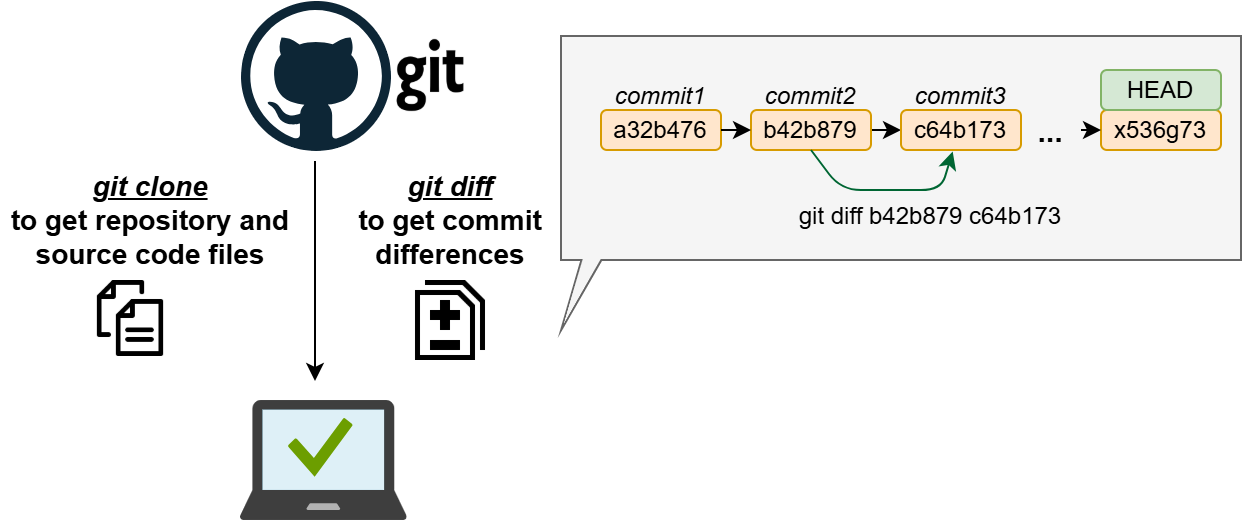
\includegraphics[width=\textwidth]{gitdata.png}
\caption{Using Git commands (\texttt{clone} and \texttt{diff}) to retrieve source code and commit changes.}
\label{fig:extracting_data_with_git}
\end{figure}


Listing \ref{lst:git_diff} provides an example of a \texttt{git diff} output for three files: \texttt{User.java}, \texttt{Calculator.java}, and \texttt{Utils.java}. From the diff output, we can identify the names of the changed files and information about added or deleted lines of code, but not the specific entities (e.g., classes or interfaces) from those files. 

To determine the changed entities, we first extract the structural dependencies of the system and create a mapping between the entities defined in each file and the file. Later, we associate the changed files with their corresponding entities when processing the diff files using this mapping \cite{DepSACI, b4, icstcc-2024, enase19}. 

For instance, in this example, the mapping can reveal that \texttt{User.java} contains the class \texttt{User}, \texttt{Calculator.java} contains the class \texttt{Calculator}, and \texttt{Utils.java} contains the class \texttt{Utils}. Even if Java typically enforces a standardized relationship between file and entity names, this is not always the case for other programming languages, so we need a uniform approach.

Using this mapping, we can say that the commit presented in Listing \ref{lst:git_diff} generates three pairs of co-changed entities: \texttt{Utils-Calculator}, \texttt{Utils-User}, and \texttt{Calculator-User}.

\begin{lstlisting}[language=diff, caption={Example output of \texttt{git diff} between two commits.}, label={lst:git_diff}]
commit 1a2b3c4d5e (HEAD -> main)
Author: Developer <developer@example.com>
Date:   Wed Dec 13 12:34:56 2024 +0000

    Refactored code and added new features.

diff --git a/src/User.java b/src/User.java
index abc1234..def5678 100644
--- a/src/User.java
+++ b/src/User.java
@@ -1,5 +1,6 @@
+    public User(String name) {
+        this.name = name;
+    }

-    public void greet() {
+    public void displayGreeting() {
         System.out.println("Hello, " + name + "!");
     }
 }

diff --git a/src/Calculator.java b/src/Calculator.java
index 9876543..2345678 100644
--- a/src/Calculator.java
+++ b/src/Calculator.java
@@ -5,7 +5,7 @@ 
-    public int subtract(int a, int b) {
+    public int subtractNumbers(int a, int b) {
         return a - b;
     }
 }

diff --git a/src/Utils.java b/src/Utils.java
index 56789ab..789abcd 100644
--- a/src/Utils.java
+++ b/src/Utils.java
@@ -3,7 +3,7 @
-    public static String getCurrentTime() {
+    public static String getFormattedTime() {
         return java.time.LocalTime.now().toString();
     }
 }
\end{lstlisting}




\section{Tool for measuring software dependencies}
\label{subsec:tool_measuring_dependencies}

\hspace{4em}To extract structural and logical dependencies, we developed a tool that takes as input the source code repository URL of a given system and extracts the corresponding software dependencies \cite{DepSACI, enase19}. 

From a workflow perspective, the tool performs three main activities: downloading the necessary data from the repository, extracting structural dependencies from the source code, and identifying and filtering co-changing pairs from the repository's commit history. Figure \ref{fig:figworkflow} illustrates these activities, with each block representing a different step from the process.


To get the source code files and the change history, we first need to know the repository URL from GitHub (GitHub is a Git repository cloud-based hosting service). With the GitHub URL and a series of Git commands, the tool can download all the necessary data for dependencies extraction.


As presented in figure \ref{fig:extracting_data_with_git}, the \textit{"git clone"} command will download a repository, including the source code files. The \textit{"git diff"} command will get the differences between two existing commits in the Git repository. 
The tool gets the Git repository and the source code files by executing the "clone" command. Afterward, it gets all the existing commits within the Git repository. The commits are ordered by date, beginning with the oldest one and ending with the most recent one. The tool executes the "diff" command between each commit and its parent (the previous commit). The "diff" command generates a text file that contains the differences between the two commits: code differences, the number of files changed and changed file names.


The first step involves downloading the source code files and change history. This requires the GitHub repository URL, as GitHub is a cloud-based hosting service for Git repositories. Using this URL and Git commands, the tool downloads all the data necessary for dependency extraction.

\begin{figure}[H]
\centering
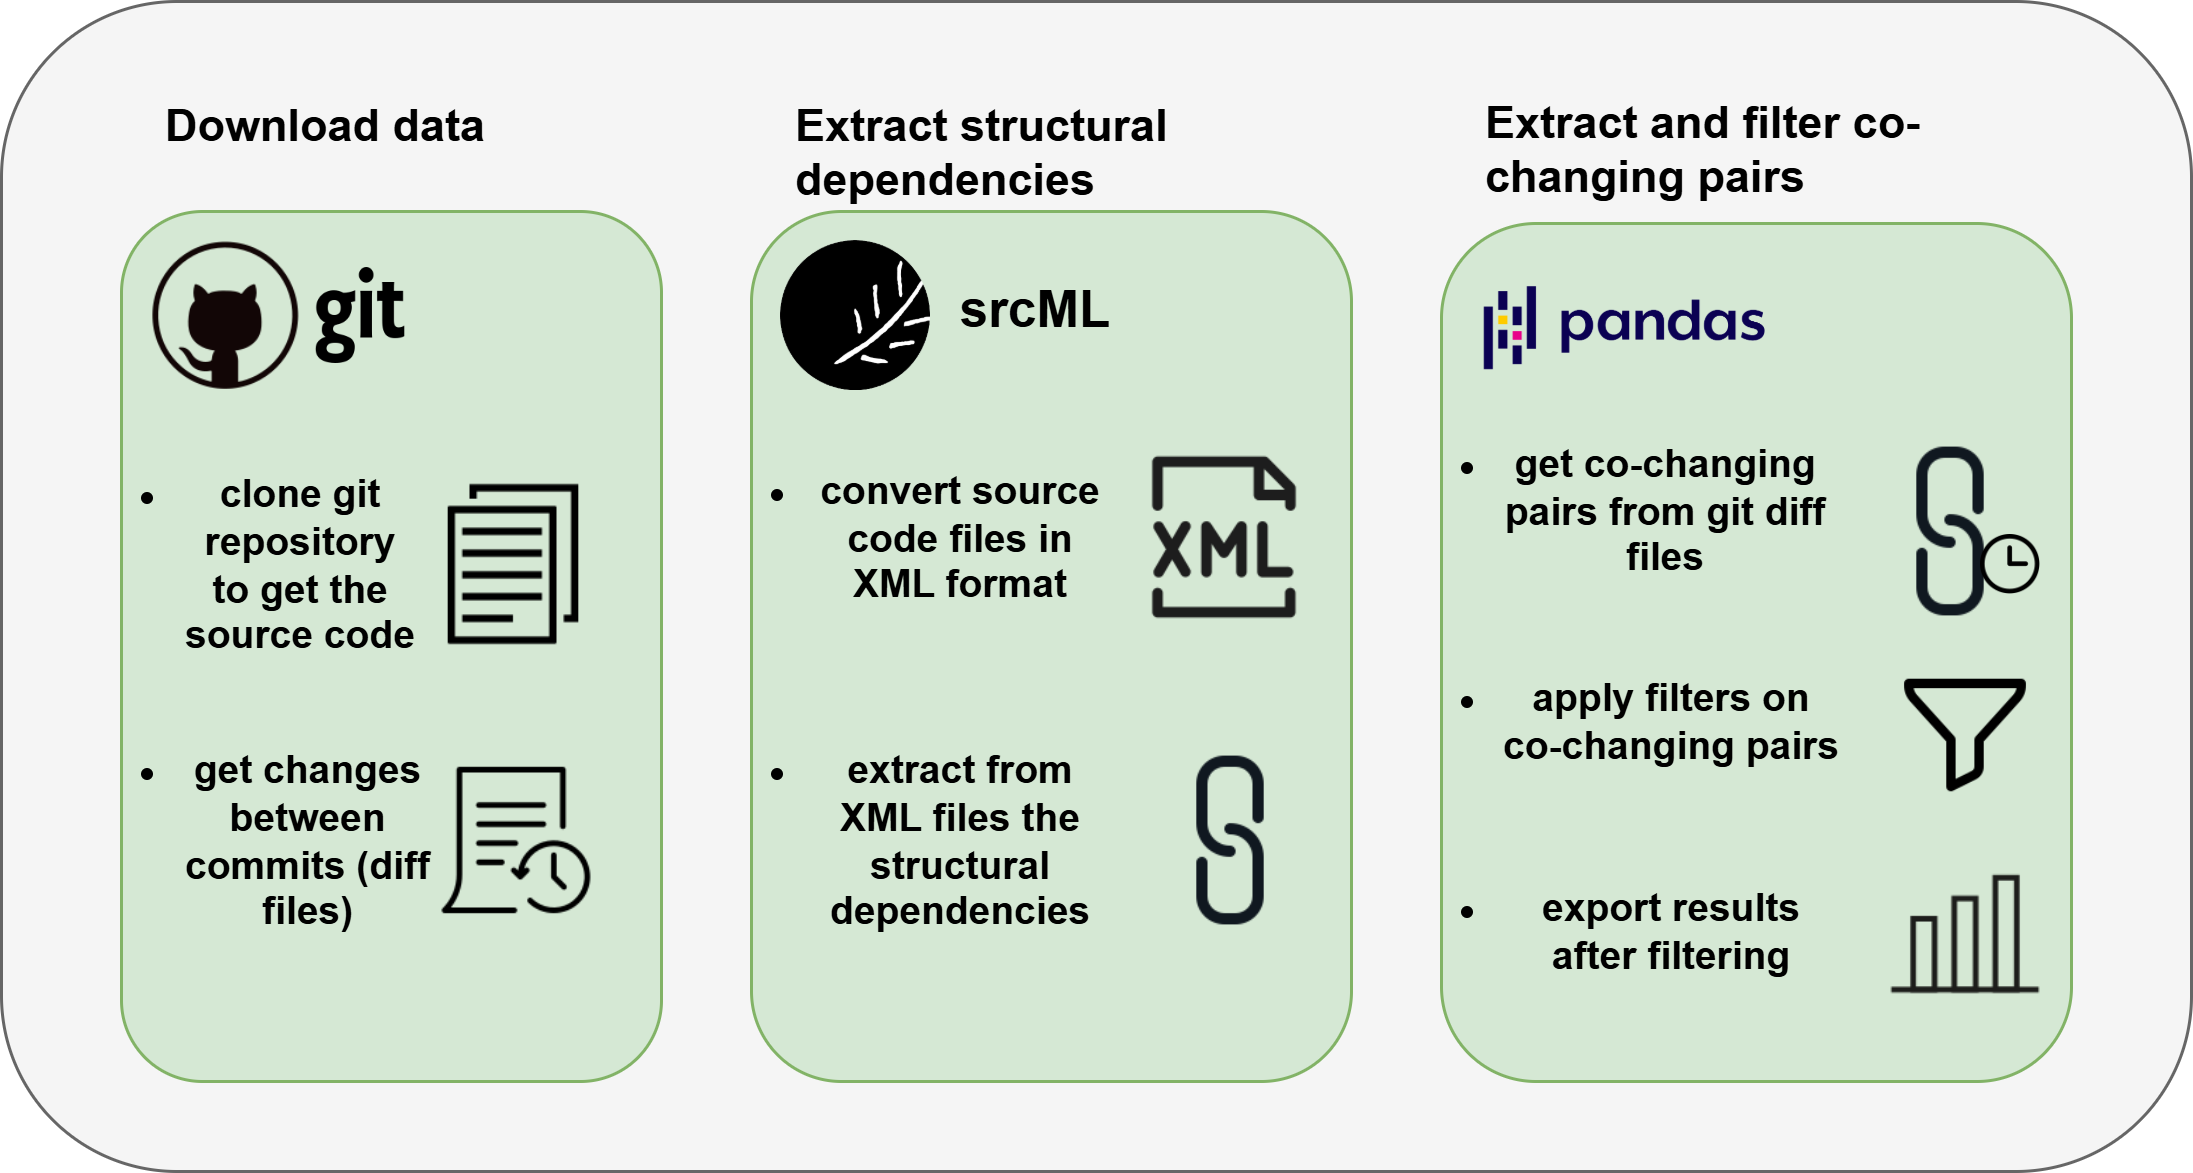
\includegraphics[width=\textwidth]{tool_workflow.png}
\caption{Tool workflow and major activities.}
\label{fig:figworkflow}
\end{figure}



\textbf{Extract structural dependencies.}

To extract structural dependencies from the source code, the tool first converts each source file into the srcML format using the method introduced in subsection \ref{subsec:extracting_structural_dependencies}. The srcML format provides an XML representation of the source code, with markup tags identifying elements of the programming language syntax\cite{srcML}. 

Once converted, the tool parses each file to identify all defined entities (such as classes, interfaces, and enums) from the file. It also detects all entities used by the defined entities. The connections between the defined and used entities form the structural dependencies.


\textbf{Extract and filter co-changing pairs.}

The process of extracting and filtering co-changing pairs is illustrated in Figure \ref{fig:figfiltering}.

To analyze the changes between commits, the tool uses the \texttt{"git diff"} command. All existing commits in the repository are collected and chronologically ordered, starting with the oldest and ending with the most recent. For each commit, the tool runs the \texttt{"git diff"} command to compare it with its parent (the preceding commit). This generates a text file containing the details of the changes between the two commits.

To extract co-changing pairs, the tool parses each generated diff file. From each file, it identifies the number of changed files and their names. Since the tool already knows the software entities contained in each file (from the structural dependencies extraction), it can determine co-changing pairs by linking entities from changed files. Once all the co-changing pairs for a diff file are extracted, the tool moves to the next diff file and repeats the process.

Explained in more detail in subsections \ref{subsec:filtering_transaction_size}, \ref{subsec:filtering_support}, \ref{subsec:filtering_connection_strength}, and \ref{subsec:filtering_comments}, not every extracted co-changing pair is considered a logical dependency. For a pair to be considered a logical dependency, it must pass some criteria. These criteria are implemented as filters in the tool. Each filter processes the extracted co-changing pairs and outputs the pairs that meet the filter requirements. The filters can also be combined to ensure that only meaningful logical dependencies remain after filtering.

\begin{figure}[H]
\centering
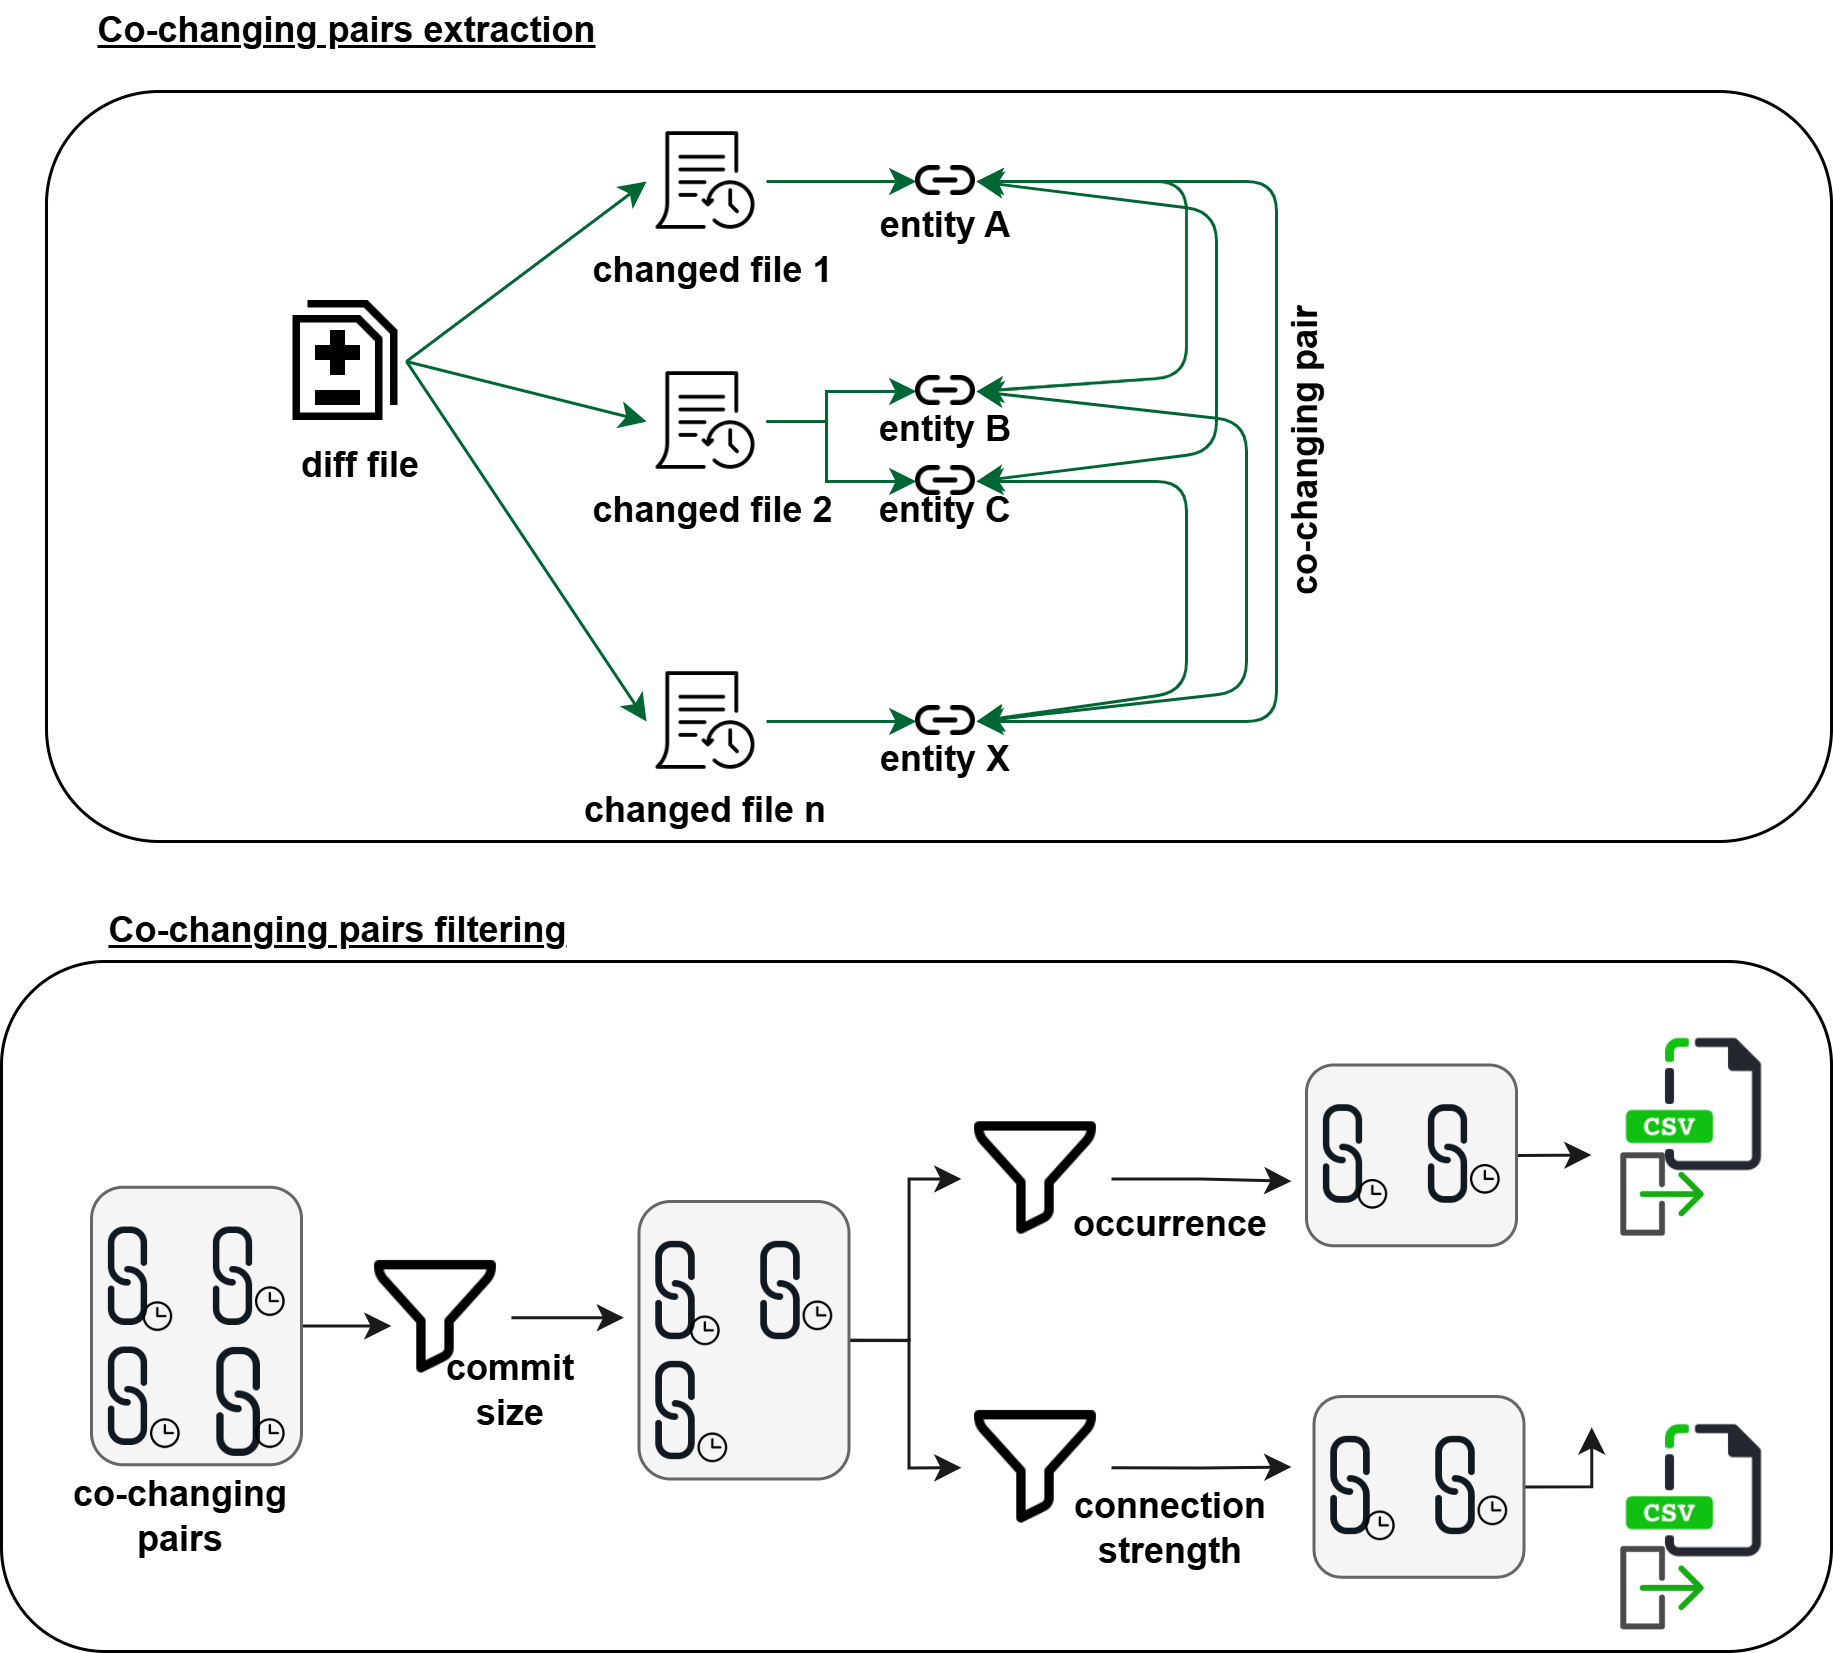
\includegraphics[width=\textwidth]{pairs_filtering.png}
\caption{Co-changing pairs extraction and filtering.}
\label{fig:figfiltering}
\end{figure}



\section{Filtering logical dependencies}
\label{sec:filtering_logical_dependencies}

\hspace{4em}As discussed in Section \ref{ld-intro}, the number of co-changing pairs extracted from software repositories can be quite large, often reaching millions. This quantity, combined with noise in the data, makes it important to apply filtering techniques to identify meaningful co-changing pairs.

This section presents three filtering techniques used to refine the extracted co-changing pairs. The filter based on commit transaction size, discussed in Section \ref{subsec:filtering_transaction_size}, is always applied. The experiments are performed by combining this filter with one of the other two filters: the support filter presented in Section \ref{subsec:filtering_support} or the connection strength filter discussed in Section \ref{subsec:filtering_connection_strength}. The commit size filter aims to reduce the overall size of the co-changing pairs, while the support and connection strength filters aim to minimize noise in the data.

\subsection{Filtering based on commit transaction size}
\label{subsec:filtering_transaction_size}

With this filtering approach, the goal is to reduce the total number of extracted co-changing pairs and move closer to identifying meaningful logical dependencies. 

Large commits often involve many files due to non-functional changes like branch merges, folder restructuring, or formatting updates. These types of commits can introduce noise by creating irrelevant co-changing pairs. Dependencies are more meaningful when extracted from commits that involve feature development or bug fixes, where developers modify related code files. However, if multiple unrelated features or fixes are solved into a single commit, it can add false relationships between the entities.

One example of this issue is the initial commit when a system is migrated to a new versioning platform. These commits typically include many files but no functional changes. Another example is merge commits, created automatically during branch integrations. These commits combine changes from multiple smaller commits, which often address different issues or features. In such cases, analyzing the smaller, individual commits provides more accurate information than the overall merge commit \cite{cluster-access}.

Different studies have used various threshold values for filtering commit sizes. Cappiluppi and Ajienka \cite{DBLP:journals/jss/AjienkaC17, DBLP:journals/ese/AjienkaCC18} only considered commits with fewer than 10 modified source code files. Similarly, Kagdi et al. used the same threshold, excluding commits with more than 10 source files. Ying et al. \cite{Ying-co-change} took a different approach, excluding commits involving over 100 files. Zimmermann et al. \cite{Zimmermann:2004:MVH:998675.999460} configured the ROSE tool to exclude commits larger than 30 files. Moonen et al. \cite{Moonen-commit} explored seven different transaction filtering sizes (2, 4, 6, 8, 10, 20, and 30), recommending a threshold of 8 files.



We analyzed the overall transaction size trend for 27 open-source C\# and Java systems with a total of 74,332 commits. The results are presented in Figure \ref{fig:fig_cs} and in Table \ref{table:cs_values}. Based on the analysis, we observed that 90\% of the total commit transactions involved fewer than 10 source code files. This percentage indicates that setting a threshold of 10 files for the maximum size of commit transactions will not affect too much the total number of commits available for extracting co-changing pairs, 90\% of the transactions still remain available for analysis \cite{DepSACI, enase19}.

Table \ref{table:cs_values} provides more details of the commit transaction size distribution for each system. The columns in the table represent the following information:

\hspace{-4em}- \textit{$cs\leq 5$}: The number of commits with a transaction size of 5 or fewer files. \\
- \textit{$cs\leq 10$}: The number of commits with a transaction size of 10 or fewer files. \\
- \textit{$cs\leq 20$}: The number of commits with a transaction size of 20 or fewer files. \\
- \textit{$cs<\infty$}: The total number of commits for the system. \\
- \textit{$Avg$}: The average transaction size for the system.


\begin{figure}[!h]
\centering
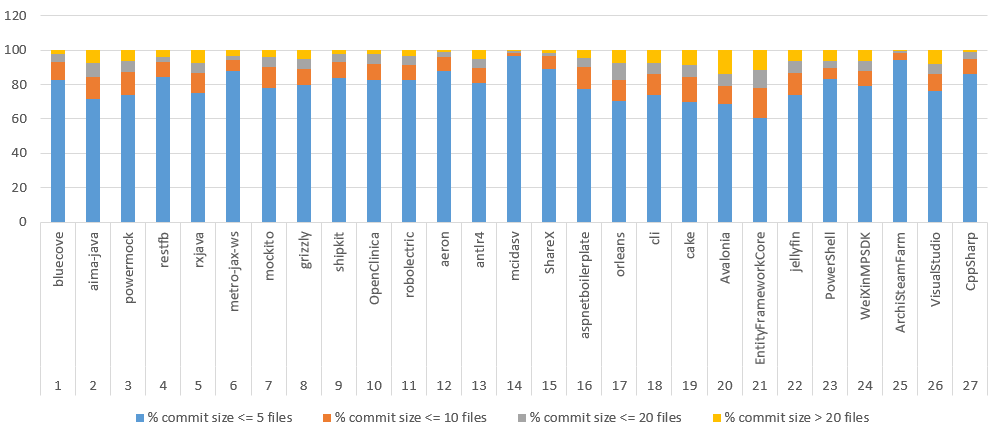
\includegraphics[width=\textwidth]{commit_distribution.png}
\caption{Commit transaction size(cs) trend in percentages.}
\label{fig:fig_cs}
\centering
\end{figure}


\begin{figure}[!h]
\centering
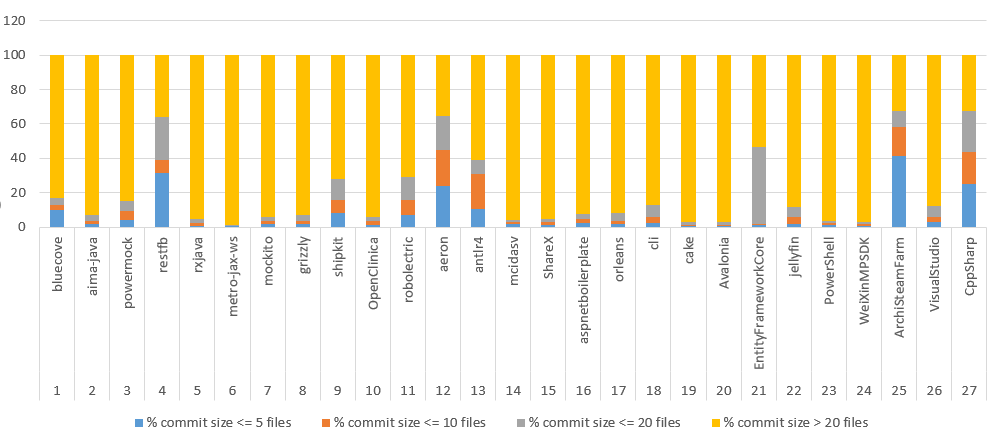
\includegraphics[width=\textwidth]{ld_distribution.png}
\caption{Percentages of co-changing pairs extracted from each commit transaction size(cs) group.}
\label{fig:fig_ld_cs}
\centering
\end{figure}

As we can see in Figure \ref{fig:fig_ld_cs}, even though only 5\% of the commit transactions have more than 20 files changed ($20<cs<\infty$), they generate, on average, 80\% of the total amount of co-changing pairs extracted from the systems.  
The high number of co-changing pairs extracted from such a small number of commit transactions is caused by the number of files involved in those commit transactions.  

One single commit transaction can lead to a large amount of co-changing pairs. For example, in RxJava, we have commit transactions with 1030 source code files. This means that those commits can generate  
\[
\Comb{n}{k}=\frac{n!}{k!(n-k)!} = \frac{1030!}{2!(1028)!} = 529 935
\]
logical dependencies. By setting a threshold on the commit transaction size, we can avoid the introduction of those co-changing pairs into the system.  

Filtering 10\% of the total amount of commit transactions can significantly decrease the number of co-changing pairs. That is why we choose the value of 10 files as our fixed threshold for the maximum size of a commit transaction \cite{DepSACI}.



\begin{table}[!h]
\renewcommand{\arraystretch}{1}
\caption{Commit transaction size(cs) trend and average per system.}
\label{table:cs_values}
\centering
\scalebox{0.9}{
\begin{tabular}{|c|c|c|c|c|c|c|}
\hline
$Nr.$	  & $Project $   &	$cs\leq 5$	&	$cs\leq 10$	&	$cs\leq 20$	&	$cs<\infty$ & Avg	\\ 
\hline
1	&	bluecove	&	738	&	97	&	37	&	22	&	4.9	\\
2	&	aima-java	&	733	&	134	&	74	&	65	&	7.24	\\
3	&	powermock	&	685	&	128	&	66	&	70	&	9.61	\\
4	&	restfb	&	1160	&	127	&	44	&	60	&	9.9	\\
5	&	rxjava	&	3395	&	447	&	253	&	303	&	8.46	\\
6	&	metro-jax-ws	&	2583	&	198	&	78	&	68	&	4.33	\\
7	&	mockito	&	2522	&	433	&	222	&	153	&	6.33	\\
8	&	grizzly	&	2487	&	302	&	180	&	144	&	5.28	\\
9	&	shipkit	&	1311	&	151	&	64	&	37	&	4.26	\\
10	&	OpenClinica	&	2837	&	250	&	119	&	70	&	3.31	\\
11	&	robolectric	&	4827	&	503	&	264	&	318	&	7.43	\\
12	&	aeron	&	4844	&	684	&	300	&	149	&	4.6	\\
13	&	antlr4	&	3426	&	437	&	304	&	264	&	8.5	\\
14	&	mcidasv	&	3996	&	81	&	35	&	24	&	2.47	\\
15	&	ShareX	&	4731	&	529	&	145	&	80	&	4.69	\\
16	&	aspnetboilerplate	&	3208	&	569	&	321	&	225	&	6.61	\\
17	&	orleans	&	2780	&	518	&	369	&	328	&	8.95	\\
18	&	cli	&	3377	&	551	&	308	&	252	&	6.43	\\
19	&	cake	&	1785	&	359	&	174	&	200	&	9.89	\\
20	&	Avalonia	&	3806	&	641	&	371	&	446	&	8.43	\\
21	&	EntityFrameworkCore	&	2866	&	878	&	644	&	822	&	15.38	\\
22	&	jellyfin	&	4007	&	662	&	419	&	345	&	6.25	\\
23	&	PowerShell	&	2702	&	224	&	133	&	191	&	7.33	\\
24	&	WeiXinMPSDK	&	4604	&	526	&	296	&	303	&	9.01	\\
25	&	ArchiSteamFarm	&	2357	&	92	&	28	&	20	&	2.24	\\
26	&	VisualStudio	&	3902	&	521	&	295	&	321	&	6.71	\\
27	&	CppSharp	&	3870	&	390	&	203	&	59	&	3.28	\\
\hline
\end{tabular}
}
\end{table}





\subsection{Filtering based on support}
\label{subsec:filtering_support}

\hspace{4em}In the previous section, we filtered the co-changing pairs based on commit size. Although this reduced the number of extracted co-changing pairs, this type of filtering does not guarantee that the remaining co-changing pairs are valid logical dependencies. A single occurrence of a co-changing pair could represent a valid logical dependency, but it could also be a coincidence.  

To address this, the \textit{support metric} is applied. The support metric of a rule $(A \rightarrow B)$, where $A$ is the antecedent and $B$ is the consequent, is defined as the number of commits (transactions) in which both entities are changed together. Many studies have used the support metric to filter logical dependencies. For example, \textit{Zimmermann et al.} \cite{Zimmermann:2004:MVH:998675.999460} applied minimum support thresholds of 1, 3, and 5 in their ROSE tool, while \textit{Kagdi et al.} \cite{article-Kagdi-commit} used thresholds of 1, 2, 4, and 8.

Considering only co-changing pairs with a minimum support threshold can help improve accuracy. However, for projects with a smaller number of commits, it becomes less likely to find co-changing pairs with high support, which could end up filtering out all the extracted co-changes.

We performed a series of analyses on the test systems, incrementing the support threshold (\textit{support}) from 1 to 4. Co-changing pairs were extracted only from commits with a transaction size of a maximum of 10 files. For each threshold mentioned above, the extracted co-changing pairs were then filtered based on the specified support threshold. Any co-changing pairs that did not meet the minimum support criteria were discarded.


Tables \ref{table:ld_ratio} and \ref{table:sd_percentages} provide detailed results for the support filtering applied to co-changing pairs. Table \ref{table:sd_percentages} presents the percentages of co-changing pairs that are also structural dependencies, and Table \ref{table:ld_ratio} presents the ratio of the number of co-changing pairs to the number of structural dependencies (SD). The columns in the tables represent the following information:

\hspace{-4em}- \textit{$Project\ nr.$}: The unique identifier assigned to each system. \\
- \textit{$support\geq 1$}: Represents the results when the minimum support threshold is set to 1, the ratio of co-changing pairs to structural dependencies (Table \ref{table:ld_ratio}) or the percentage of co-changing pairs that are also structural dependencies (Table \ref{table:sd_percentages}). \\
- \textit{$support\geq 2$}: Represents the results when the minimum support threshold is set to 2. \\
- \textit{$support\geq 3$}: Represents the results when the minimum support threshold is set to 3. \\
- \textit{$support\geq 4$}: Represents the results when the minimum support threshold is set to 4.


\begin{table}[!h]
\renewcommand{\arraystretch}{1}
\caption{Percentage of co-changing pairs that are also structural dependencies.}
\label{table:sd_percentages}
\centering
\scalebox{0.9}{
\begin{tabular}{|c|c|c|c|c|}
\hline
$Project\ nr.$ & $support\geq 1$ & $support\geq 2$ & $support\geq 3$ & $support\geq 4$  \\
\hline
1	&	7,13	&	7,77	&	7,99	&	19,71	\\
2	&	19,54	&	25,76	&	29,55	&	32,16	\\
3	&	6,66	&	8,58	&	11,82	&	14,87	\\
4	&	1,16	&	1,17	&	0,91	&	0,80	\\
5	&	3,99	&	3,96	&	7,75	&	7,49	\\
6	&	13,92	&	20,16	&	22,91	&	22,77	\\
7	&	8,38	&	9,28	&	14,93	&	14,58	\\
8	&	6,70	&	9,73	&	14,20	&	15,60	\\
9	&	16,98	&	23,34	&	29,22	&	32,89	\\
10	&	8,94	&	9,15	&	11,05	&	10,59	\\
11	&	4,99	&	6,92	&	8,88	&	11,08	\\
12	&	13,19	&	17,15	&	18,60	&	19,57	\\
13	&	2,43	&	5,59	&	8,33	&	8,21	\\
14	&	13,27	&	18,88	&	19,02	&	19,28	\\
15	&	12,90	&	21,95	&	25,51	&	27,01	\\
16	&	13,33	&	17,34	&	18,53	&	16,24	\\
17	&	6,09	&	6,18	&	6,41	&	6,44	\\
18	&	9,73	&	10,60	&	14,27	&	18,80	\\
19	&	10,26	&	13,54	&	13,64	&	12,60	\\
20	&	12,83	&	18,36	&	21,00	&	25,72	\\
21	&	2,86	&	4,65	&	5,70	&	4,98	\\
22	&	5,20	&	6,56	&	8,18	&	8,90	\\
23	&	8,23	&	13,64	&	17,04	&	17,65	\\
24	&	6,77	&	10,89	&	14,47	&	16,05	\\
25	&	9,85	&	10,15	&	11,65	&	11,33	\\
26	&	8,65	&	10,79	&	12,78	&	14,34	\\
27	&	7,04	&	8,78	&	9,87	&	10,08	\\
\hline
Avg	&	8,93	&	11,88	&	14,23	&	15,55	\\
\hline
\end{tabular}
}
\end{table}


\begin{table}[!h]
\renewcommand{\arraystretch}{1}
\caption{Ratio of number of co-changing pairs to number of structural dependencies. }
\label{table:ld_ratio}
\centering
\scalebox{0.9}{
\begin{tabular}{|c|c|c|c|c|}
\hline
$Project\ nr.$  & $support\geq 1$ & $support\geq 2$ & $support\geq 3$ & $support\geq 4$  \\
\hline
1	&	4,13	&	1,94	&	1,23	&	0,26	\\
2	&	0,81	&	0,33	&	0,16	&	0,10	\\
3	&	5,12	&	1,93	&	0,78	&	0,38	\\
4	&	53,36	&	42,00	&	38,31	&	36,30	\\
5	&	4,27	&	2,90	&	0,88	&	0,72	\\
6	&	1,07	&	0,46	&	0,30	&	0,23	\\
7	&	4,09	&	2,38	&	0,99	&	0,73	\\
8	&	4,06	&	1,57	&	0,76	&	0,49	\\
9	&	3,64	&	2,03	&	1,14	&	0,77	\\
10	&	1,41	&	1,01	&	0,47	&	0,34	\\
11	&	7,91	&	4,47	&	2,93	&	2,03	\\
12	&	3,92	&	2,15	&	1,47	&	1,07	\\
13	&	10,15	&	3,18	&	1,22	&	1,03	\\
14	&	3,07	&	1,53	&	1,16	&	0,97	\\
15	&	2,34	&	0,84	&	0,48	&	0,33	\\
16	&	1,21	&	0,47	&	0,26	&	0,19	\\
17	&	2,99	&	1,83	&	1,11	&	0,84	\\
18	&	2,26	&	1,37	&	0,67	&	0,40	\\
19	&	2,32	&	1,38	&	0,76	&	0,67	\\
20	&	1,24	&	0,58	&	0,35	&	0,18	\\
21	&	5,33	&	2,12	&	1,27	&	1,05	\\
22	&	3,38	&	1,88	&	0,99	&	0,74	\\
23	&	3,62	&	1,22	&	0,76	&	0,37	\\
24	&	2,57	&	1,22	&	0,67	&	0,46	\\
25	&	7,47	&	5,36	&	4,16	&	3,73	\\
26	&	4,03	&	2,16	&	1,50	&	1,15	\\
27	&	7,46	&	4,26	&	2,99	&	2,43	\\
\hline
Avg	&	5,67	&	3,43	&	2,51	&	2,15	\\
\hline
\end{tabular}
}
\end{table}
Based on Table \ref{table:sd_percentages}, we observe that only a small percentage of the extracted co-changing pairs overlap with structural dependencies. This observation is consistent with findings from related works \cite{DBLP:journals/jss/AjienkaC17, DBLP:journals/ese/AjienkaCC18}. The percentage of co-changing pairs that are structural dependencies increases as the minimum support threshold rises.

We calculate the overlap between co-changing pairs and structural dependencies not only to understand how many structural dependencies are reflected in the versioning system through co-changing pairs but also to filter out co-changing pairs that are structural dependencies, as they do not provide new information about the system.

We stopped the minimum support threshold at 4 because, as observed in Table \ref{table:ld_ratio}, systems with IDs 2, 6, 10, and 16 show a ratio below 1, indicating that the number of structural dependencies exceeds the number of co-changing pairs. For systems with IDs 4, 11, 25, and 27, increasing the threshold to 4 does not significantly reduce the difference between the number of co-changing pairs and structural dependencies.

Raising the support threshold beyond 4 might cause filtering out all co-changing pairs for some systems. Therefore, while applying a threshold of 4 filters co-changing pairs to identify logical dependencies, the remaining number of co-changing pairs still significantly exceeds the number of structural dependencies for certain systems.


\subsection{Filtering based on connection strength}
\label{subsec:filtering_connection_strength}

\hspace{4em}In Section \ref{subsec:filtering_transaction_size}, we applied a filtering rule to exclude co-changing pairs extracted from commits involving more than 10 changed files. This decision was based on the results obtained from analyzing the commit size.

In Section \ref{subsec:filtering_support}, we introduced an additional filter based on the support metric of a co-changing pair. This filter was applied after the commit size filter. However, the results highlighted a challenge: using a fixed threshold for filtering may not be effective across systems of varying sizes. A threshold that works well for smaller systems may need to be increased for medium-sized systems and vice versa.

To address this issue, we introduced another filter complementary to the commit size filter described in Section \ref{subsec:filtering_transaction_size}. This new filter focuses on the connection strength of co-changing pairs. A co-changing pair that appears only once in a system's history may be less reliable than one that occurs more frequently \cite{cluster-access}.

Zimmermann et al. proposed the support and confidence metrics to measure the reliability of co-changes \cite{Zimmermann:2004:MVH:998675.999460}.

The \textit{support metric} for a rule $(A \rightarrow B)$, where A is the antecedent, and B is the consequent, is defined as the number of commits (transactions) in which both entities are modified together.

The \textit{confidence metric} of the same rule $(A \rightarrow B)$, as expressed in Equation \eqref{eq:confidence}, measures the proportion of commits involving both entities relative to the total number of commits where A appears.

\[
\text{$confidence$}(A \rightarrow B) = \frac{\text{$Nr.\ of\ commits\ containing$} A \text{ $and$ } B}{\text{$Nr.\ of\ commits\ containing$ } A}
\tag{\ref{eq:confidence}}
\]



The confidence metric focuses on entities that are modified less frequently but consistently together, rather than entities that are modified more often but with multiple other entities.

For example, assuming that entity \( A \) was changed in 10 commits and, of these 10 commits, 9 also included changes to entity \( B \), the confidence for the rule \( (A \rightarrow B) \) would be 0.9. On the other hand, if entity \( C \) was changed in 100 commits and, of these 100 commits, 50 also included changes to entity \( D \), the confidence for the rule \( (C \rightarrow D) \) would be 0.5. This means we would have more confidence in the first pair \( (A \rightarrow B) \) than in the second pair \( (C \rightarrow D) \), even though the second pair has more than five times the number of updates together \cite{cluster-access}.


This observation was also made by \textit{Ying et al.} \cite{Ying-co-change}, who analyzed co-change patterns to recommend potentially relevant source code to developers during development tasks. In their study, they did not use the confidence metric, as they considered it misleading when some files are changed much more frequently than others. Instead, they used only support thresholds from 5 to 30.
 

To favor entities that frequently appear in commits together, we calculated a \textit{system factor}. This factor represents the average support metric value for all entity pairs within the system \cite{cluster-access}.

The system factor is then incorporated into the confidence metric calculation by multiplying the two values. To ensure the metric can also serve as a weight alongside structural dependency weights, we scale the resulting value by 100 to make it supraunitary and limit the range between 0 and 100.

This modified formula is referred to as the strength metric, which is defined in Equation \eqref{eq:strength}.

\begin{equation}
\text{$strength$}(A \rightarrow B) = \text{$confidence$}(A \rightarrow B) \times 100 \times \text{$system\ factor$}
\label{eq:strength}
\end{equation}



\begin{table}[!h]
\renewcommand{\arraystretch}{1}
\caption{Ratio of number of filtered co-changing pairs to number of structural dependencies, when strength A and strength B $\geq threshold \%$}
\label{tab:commitstrengthAND}
\centering
\scalebox{0.8}{
\begin{tabular}{|c|cccccccccc|c|}
\hline
$Project\ nr.$  & $\geq10\%$ & $\geq20\%$ & $\geq30\%$ & $\geq40\%$ & $\geq50\%$ & $\geq60\%$ & $\geq70\%$ & $\geq80\%$ & $\geq90\%$ & $\geq100\%$ \\
\hline
1  & 1.326 & 0.658 & 0.433 & 0.401 & 0.244 & 0.199 & 0.195 & 0.022 & 0.011 & 0.011 \\
2  & 0.266 & 0.137 & 0.070 & 0.044 & 0.036 & 0.019 & 0.005 & 0.004 & 0.003 & 0.003 \\
3  & 0.505 & 0.243 & 0.147 & 0.086 & 0.061 & 0.031 & 0.031 & 0.031 & 0.031 & 0.031 \\
4  & 0.822 & 0.163 & 0.045 & 0.017 & 0.011 & 0.002 & 0.001 & 0.001 & 0.001 & 0.001 \\
5  & 0.234 & 0.119 & 0.054 & 0.037 & 0.034 & 0.018 & 0.013 & 0.011 & 0.007 & 0.007 \\
6  & 0.227 & 0.155 & 0.101 & 0.077 & 0.070 & 0.036 & 0.018 & 0.017 & 0.016 & 0.016 \\
7  & 1.590 & 0.804 & 0.357 & 0.288 & 0.215 & 0.088 & 0.052 & 0.036 & 0.032 & 0.032 \\
8  & 2.073 & 0.293 & 0.170 & 0.111 & 0.093 & 0.050 & 0.039 & 0.034 & 0.021 & 0.007 \\
9  & 1.495 & 0.479 & 0.271 & 0.142 & 0.108 & 0.059 & 0.047 & 0.011 & 0.008 & 0.008 \\
10 & 0.253 & 0.135 & 0.093 & 0.078 & 0.062 & 0.042 & 0.024 & 0.019 & 0.019 & 0.017 \\
11 & 0.114 & 0.086 & 0.064 & 0.037 & 0.027 & 0.025 & 0.001 & 0.000 & 0.000 & 0.000 \\
12 & 0.277 & 0.136 & 0.085 & 0.069 & 0.053 & 0.045 & 0.039 & 0.015 & 0.007 & 0.004 \\
13 & 11.363 & 0.721 & 0.031 & 0.010 & 0.007 & 0.004 & 0.000 & 0.000 & 0.000 & 0.000 \\
14 & 3.225 & 0.805 & 0.660 & 0.533 & 0.493 & 0.454 & 0.386 & 0.356 & 0.005 & 0.005 \\
15 & 6.097 & 0.725 & 0.663 & 0.564 & 0.500 & 0.242 & 0.176 & 0.170 & 0.001 & 0.001 \\
16 & 1.302 & 0.333 & 0.219 & 0.146 & 0.094 & 0.045 & 0.014 & 0.008 & 0.007 & 0.007 \\
17 & 0.816 & 0.640 & 0.551 & 0.503 & 0.496 & 0.196 & 0.159 & 0.152 & 0.142 & 0.142 \\
18 & 1.676 & 0.233 & 0.159 & 0.118 & 0.102 & 0.062 & 0.058 & 0.029 & 0.026 & 0.026 \\
19 & 2.335 & 0.753 & 0.614 & 0.337 & 0.075 & 0.021 & 0.007 & 0.004 & 0.004 & 0.004 \\
20 & 0.846 & 0.117 & 0.098 & 0.018 & 0.013 & 0.002 & 0.001 & 0.001 & 0.001 & 0.001 \\
21 & 3.377 & 1.691 & 1.608 & 1.584 & 1.576 & 1.310 & 0.001 & 0.001 & 0.001 & 0.001 \\
22 & 0.132 & 0.006 & 0.003 & 0.002 & 0.002 & 0.000 & 0.000 & 0.000 & 0.000 & 0.000 \\
23 & 1.732 & 1.299 & 0.158 & 0.053 & 0.007 & 0.001 & 0.000 & 0.000 & 0.000 & 0.000 \\
24 & 3.295 & 0.334 & 0.188 & 0.061 & 0.017 & 0.006 & 0.003 & 0.001 & 0.000 & 0.000 \\
25 & 0.897 & 0.479 & 0.429 & 0.423 & 0.412 & 0.403 & 0.339 & 0.009 & 0.001 & 0.000 \\
26 & 1.281 & 0.090 & 0.053 & 0.028 & 0.020 & 0.013 & 0.006 & 0.001 & 0.001 & 0.001 \\
27 & 99.528 & 1.020 & 0.992 & 0.980 & 0.972 & 0.927 & 0.078 & 0.075 & 0.073 & 0.072 \\
\hline
\end{tabular}
}
\end{table}



\begin{table}[!h]
\renewcommand{\arraystretch}{1}
\caption{Ratio of number of filtered co-changing pairs to number of structural dependencies, when strength A or strength B $\geq threshold \%$}
\label{tab:commitstrengthOR}
\centering
\scalebox{0.8}{
\begin{tabular}{|c|cccccccccc|c|}
\hline
$Project\ nr.$ & $\geq10\%$ & $\geq20\%$ & $\geq30\%$ & $\geq40\%$ & $\geq50\%$ & $\geq60\%$ & $\geq70\%$ & $\geq80\%$ & $\geq90\%$ & $\geq100\%$ \\
\hline
1  & 1.312 & 1.181 & 0.700 & 0.599 & 0.419 & 0.235 & 0.219 & 0.046 & 0.045 & 0.045 \\
2  & 0.430 & 0.280 & 0.176 & 0.118 & 0.103 & 0.056 & 0.022 & 0.020 & 0.020 & 0.020 \\
3  & 0.508 & 0.328 & 0.234 & 0.179 & 0.150 & 0.092 & 0.091 & 0.091 & 0.091 & 0.091 \\
4  & 0.662 & 0.336 & 0.122 & 0.067 & 0.059 & 0.016 & 0.015 & 0.015 & 0.015 & 0.015 \\
5  & 0.279 & 0.206 & 0.145 & 0.100 & 0.099 & 0.047 & 0.044 & 0.039 & 0.034 & 0.034 \\
6  & 0.271 & 0.261 & 0.204 & 0.172 & 0.160 & 0.106 & 0.082 & 0.081 & 0.080 & 0.080 \\
7  & 2.481 & 1.521 & 0.904 & 0.623 & 0.411 & 0.199 & 0.128 & 0.107 & 0.101 & 0.101 \\
8  & 1.332 & 0.838 & 0.515 & 0.320 & 0.288 & 0.142 & 0.117 & 0.106 & 0.090 & 0.076 \\
9  & 1.376 & 1.083 & 0.725 & 0.515 & 0.424 & 0.191 & 0.149 & 0.105 & 0.094 & 0.094 \\
10 & 0.830 & 0.434 & 0.314 & 0.256 & 0.217 & 0.130 & 0.093 & 0.082 & 0.080 & 0.072 \\
11 & 0.366 & 0.122 & 0.088 & 0.046 & 0.031 & 0.027 & 0.003 & 0.002 & 0.002 & 0.002 \\
12 & 0.781 & 0.449 & 0.265 & 0.190 & 0.160 & 0.096 & 0.062 & 0.031 & 0.021 & 0.018 \\
13 & 11.363 & 0.798 & 0.055 & 0.022 & 0.011 & 0.007 & 0.002 & 0.002 & 0.002 & 0.002 \\
14 & 1.932 & 1.203 & 0.858 & 0.682 & 0.579 & 0.473 & 0.396 & 0.365 & 0.013 & 0.013 \\
15 & 2.681 & 1.292 & 0.916 & 0.730 & 0.593 & 0.287 & 0.210 & 0.201 & 0.017 & 0.017 \\
16 & 1.055 & 0.759 & 0.493 & 0.364 & 0.273 & 0.130 & 0.067 & 0.050 & 0.046 & 0.046 \\
17 & 1.120 & 0.962 & 0.849 & 0.750 & 0.744 & 0.559 & 0.482 & 0.476 & 0.466 & 0.466 \\
18 & 1.676 & 0.762 & 0.560 & 0.434 & 0.375 & 0.269 & 0.237 & 0.149 & 0.142 & 0.142 \\
19 & 1.883 & 1.197 & 1.001 & 0.541 & 0.185 & 0.103 & 0.019 & 0.013 & 0.013 & 0.013 \\
20 & 0.510 & 0.224 & 0.138 & 0.037 & 0.028 & 0.011 & 0.006 & 0.003 & 0.003 & 0.003 \\
21 & 2.636 & 1.888 & 1.695 & 1.623 & 1.608 & 1.317 & 0.006 & 0.006 & 0.006 & 0.006 \\
22 & 0.132 & 0.030 & 0.016 & 0.011 & 0.008 & 0.003 & 0.002 & 0.002 & 0.002 & 0.002 \\
23 & 3.454 & 1.648 & 0.232 & 0.081 & 0.021 & 0.004 & 0.003 & 0.003 & 0.003 & 0.003 \\
24 & 1.342 & 0.603 & 0.327 & 0.144 & 0.080 & 0.047 & 0.015 & 0.008 & 0.007 & 0.007 \\
25 & 5.472 & 1.416 & 0.830 & 0.677 & 0.575 & 0.450 & 0.353 & 0.023 & 0.016 & 0.014 \\
26 & 1.281 & 0.236 & 0.142 & 0.092 & 0.060 & 0.040 & 0.031 & 0.020 & 0.019 & 0.019 \\
27 & 55.038 & 1.343 & 1.106 & 1.044 & 1.030 & 0.983 & 0.449 & 0.443 & 0.441 & 0.439 \\
\hline
\end{tabular}
}
\end{table}

In Table \ref{tab:commitstrengthOR}, the columns represent the ratio between the number of structural dependencies and the number of co-changing pairs that remain after filtering out pairs where at least one factor falls below the specified threshold in the column header.
In Table \ref{tab:commitstrengthAND}, the columns represent the ratio between the number of structural dependencies and the number of co-changing pairs that remain after filtering out pairs where both factors fall below the specified threshold in the column header.

We calculate this ratio between co-changing pairs and structural dependencies to assess the size of the extracted co-changing pairs compared to the structural dependencies in the system. According to surveys \cite{Shtern:2012:CMS:2332427.2332428}, \cite{sar}, the primary reason logical dependencies (i.e., filtered co-changes) are not used together with structural dependencies is their size. Therefore, it is important to evaluate the ratio between the sizes of co-changes and structural dependencies at each filtering step.

The results in Tables \ref{tab:commitstrengthAND} and \ref{tab:commitstrengthOR} show that the number of co-changing pairs is reduced. In most cases, the number of structural dependencies exceeds the number of co-changing pairs after filtering. However, the goal of filtering is not just to reduce the size of co-changing pairs but to ensure that the remaining co-changing pairs truly indicate logical dependencies.

We keep a manageable number of co-changing pairs by filtering out all co-changing pairs that do not co-occur at least 50\% of the time (factor A and factor B $\geq 50\%$). Considering both the output size and the connection strength of these pairs, the remaining co-changing pairs can be regarded as logical dependencies at this stage.



\subsection{Filtering based on code comments changes}
\label{subsec:filtering_comments}

\hspace{4em}Code comment changes are not directly related to the functional aspects of the source code, as they do not affect the system's behavior. These changes can be classified as non-functional modifications, similar to formatting.

Comment changes are visible in the diff files generated. When parsing the diff files to extract co-changes, detecting whether a change impacts only comments or involves actual source code modifications is straightforward. In this way, we can evaluate whether filtering out comment-only modifications influences the overall results. To assess the influence of code comment changes on logical dependencies, we compared two scenarios:

\hspace{-4em}- \textit{With comments}: Changes in source code files are considered, even if the modifications are only within comments. \\  
- \textit{Without comments}: Changes in source code files are ignored if they involve only editing comments.  

\hspace{-4em}In all cases, the following threshold values were varied: \\  
- \textit{Commit size} ($cs$): The maximum size of commit transactions that are accepted to generate co-changes. The values for this threshold were 5, 10, 20, and no threshold (infinity). \\  
- \textit{Support}: The minimum number of repeated occurrences (support) for a co-change to be considered a logical dependency. The values for this threshold were 1, 2, 3, and 4.  

\hspace{-4em}The six tables below present a summary of our experiments. We have computed the following values: \\  
- The mean ratio of the number of co-changes to the number of structural dependencies (SD). \\  
- The mean percentage of structural dependencies that are also co-changes (calculated as the number of overlaps divided by the number of structural dependencies). \\  
- The mean percentage of co-changes that are also structural dependencies (calculated as the number of overlaps divided by the number of co-changes).  



\begin{table}[!h]
\renewcommand{\arraystretch}{1}
\caption{Ratio of co-changes to structural dependencies (SD) with comments included, for varying commit size ($cs$) and support thresholds.}
\label{tab:ratio:comm}
\centering
\begin{tabular}{|c|c|c|c|c|}
\hline
$condition$	      &	$cs\leq 5$	&	$cs\leq 10$	&	$cs\leq 20$	&	$cs<\infty$	\\
\hline
$support\geq 1$	&	3,39	&	5,67	&	9,00	&	80,31	\\
$support\geq 2$	&	2,24	&	3,47	&	5,02	&	60,14	\\
$support\geq 3$	&	1,04	&	2,53	&	3,52	&	44,68	\\
$support\geq 4$	&	0,90	&	2,16	&	2,88	&	33,47	\\
\hline
\end{tabular}
\end{table}

\begin{table}[!h]
\renewcommand{\arraystretch}{1}
\caption{Ratio of co-changes to structural dependencies (SD) without comments, for varying commit size ($cs$) and support thresholds.}
\label{tab:ratio:nocomm}
\centering
\begin{tabular}{|c|c|c|c|c|}
\hline
$condition$	      &	$cs\leq 5$	&	$cs\leq 10$	&	$cs\leq 20$	&	$cs< \infty$	\\
\hline
$support\geq 1$	&	3,24	&	5,33	&	7,90	&	67,16	\\
$support\geq 2$	&	1,35	&	3,27	&	4,72	&	47,39	\\
$support\geq 3$	&	1,00	&	1,67	&	2,49	&	32,39	\\
$support\geq 4$	&	0,43	&	1,26	&	1,93	&	22,15	\\
\hline
\end{tabular}
\end{table}

\begin{table}[!h]
\renewcommand{\arraystretch}{1}
\caption{Percentage of structural dependencies (SD) that are also co-changes with comments included, for varying commit size ($cs$) and support thresholds.}
\label{tab:percSD:comm}
\centering
\begin{tabular}{|c|c|c|c|c|}
\hline
$condition$	      &	$cs\leq 5$	&	$cs\leq 10$	&	$cs\leq 20$	&	$cs< \infty$	\\
\hline
$support\geq 1$	&	19,75	&	29,86	&	39,29	&	76,59	\\
$support\geq 2$	&	12,50	&	20,20	&	27,68	&	66,11	\\
$support\geq 3$	&	8,49	&	14,22	&	19,94	&	55,99	\\
$support\geq 4$	&	6,58	&	10,95	&	15,76	&	47,12	\\
\hline
\end{tabular}
\end{table}

\begin{table}[!h]
\renewcommand{\arraystretch}{1}
\caption{Percentage of structural dependencies (SD) that are also co-changes without comments, for varying commit size ($cs$) and support thresholds.}
\label{tab:percSD:nocomm}
\centering
\begin{tabular}{|c|c|c|c|c|}
\hline
$condition$	      &	$cs\leq 5$	&	$cs\leq 10$	&	$cs\leq 20$	&	$cs< \infty$	\\
\hline
$support\geq 1$	&	18,88	&	28,47	&	37,44	&	71,12	\\
$support\geq 2$	&	11,87	&	19,03	&	25,93	&	59,58	\\
$support\geq 3$	&	8,00	&	13,09	&	18,15	&	48,65	\\
$support\geq 4$	&	5,85	&	9,94	&	14,27	&	39,07	\\
\hline
\end{tabular}
\end{table}

\begin{table}[!h]
\renewcommand{\arraystretch}{1}
\caption{Percentage of co-changes that are also structural dependencies (SD) with comments included, for varying commit size ($cs$) and support thresholds.}
\label{tab:percLD:comm}
\centering
\begin{tabular}{|c|c|c|c|c|}
\hline
$condition$	      &	$cs\leq 5$	&	$cs\leq 10$	&	$cs\leq 20$	&	$cs< \infty$	\\
\hline
$support\geq 1$	&	12,02	&	8,86	&	6,72	&	1,79	\\
$support\geq 2$	&	15,05	&	11,71	&	9,38	&	2,21	\\
$support\geq 3$	&	17,45	&	13,97	&	11,57	&	2,86	\\
$support\geq 4$	&	18,96	&	15,28	&	12,94	&	3,67	\\
\hline
\end{tabular}
\end{table}

\begin{table}[!h]
\renewcommand{\arraystretch}{1}
\caption{Percentage of co-changes that are also structural dependencies (SD) without comments, for varying commit size ($cs$) and support thresholds.}
\label{tab:percLD:nocomm}
\centering
\begin{tabular}{|c|c|c|c|c|}
\hline
$condition$      &	$cs\leq 5$	&	$cs\leq 10$	&	$cs\leq 20$	&	$cs< \infty$	\\
\hline
$support\geq 1$	&	12,05	&	9,02	&	6,98	&	1,93	\\
$support\geq 2$	&	15,08	&	12,03	&	9,66	&	2,42	\\
$support\geq 3$	&	17,78	&	14,37	&	12,24	&	3,28	\\
$support\geq 4$	&	19,22	&	15,59	&	13,30	&	4,21	\\
\hline
\end{tabular}
\end{table}

In all six tables (\ref{tab:ratio:comm}, \ref{tab:ratio:nocomm}, \ref{tab:percSD:comm}, \ref{tab:percSD:nocomm}, \ref{tab:percLD:comm}, \ref{tab:percLD:nocomm}), the columns represent the values used for the commit size threshold $cs$, while the rows represent the values for the support threshold $support$. The tables display median values obtained from experiments conducted under all combinations of the two thresholds across all test systems. In each table, the upper-right corner corresponds to the most relaxed filtering conditions, and the lower-left corner represents the most restrictive filtering conditions.

In order to evaluate the influence of comments, we compare pairwise Tables \ref{tab:ratio:comm} and \ref{tab:ratio:nocomm}, Tables \ref{tab:percSD:comm} and \ref{tab:percSD:nocomm} and Tables \ref{tab:percLD:comm} and \ref{tab:percLD:nocomm}. 
The comparison reveals that comment-only changes slightly increase the size of co-changing pairs with minimal impact on the overlap with structural dependencies across different thresholds. The differences between results with and without comments are more noticeable under relaxed conditions, such as ($support \geq 1$) and ($cs < \infty$). However, as the thresholds become stricter, these differences become negligible.
Excluding comments would add unnecessary complexity and increase runtime for the analysis. Due to this, we choose to include comments in the analysis for performance reasons, as their impact on the final results is minimal.



\subsection{Filtering recomandations}
\label{filtering_recomandations}

\noindent
\fbox{
\parbox{0.98\textwidth}{
- \textit{\textbf{Commit size threshold ($cs \leq 10$):}} \\  
Filtering out commits with more than 10 changed files helps reduce noise. This threshold, supported by our experiments and prior studies, filters out only a small percentage of the total commits. Our analysis shows that over 90\% of commits involve 10 or fewer files, meaning the majority of commits remain available for extracting logical dependencies.

\vspace{0.3em}

- \textit{\textbf{Include changes in code comments:}} \\  
Our analysis shows that ignoring comment-only changes has minimal impact on the results. Considering these changes simplifies the process and avoids unnecessary filtering.

\vspace{0.3em}

- \textit{\textbf{Connection strength filtering:}} \\  
This method identifies entities that co-change frequently, prioritizing stronger co-changes over incidental ones. Although a fixed threshold is not yet defined, connection strength filtering has proven to be more reliable than support filtering.
}}

%%%%%%%%%%%%%%%%%%%%%%%%%%%%%%%%%%%%%%%%%%%%%%%%%%%%%%%%%%%%%%%%%%%%%%%%%

\chapter{Combining structural and logical dependencies}
\label{chap:combining_dependencies}


\section{Overlaps between structural and logical dependencies}
\label{sec:dependency_overlaps}

\hspace{4em}A logical dependency can also be a structural dependency and vice versa. Therefore, studying the overlap between logical and structural dependencies during filtering is important, especially when the plan is to combine them for tasks such as key class detection and software clustering for architectural reconstruction. A significant overlap in this case could raise questions about whether logical dependencies provide much new information about the system.
Several studies have shown that the overlap between logical and structural dependencies is relatively small, with and without filtering \cite{DBLP:journals/jss/AjienkaC17}. This suggests that many unrelated entities are updated together in the versioning system \cite{enase19, cluster-access}.

The overlap between structural dependencies and co-changes is defined as the number of pairs that have both types of relationships: structural and logical dependencies. This overlap is analyzed in two ways:
\hspace{-4em}- \textit{as a percentage relative to the number of structural dependencies (SD).}
- \textit{as a percentage relative to the number of co-changes.}

The connection strength filtering was applied in addition to a fixed commit size threshold of \(cs \leq 10\) under two conditions:   

\hspace{-4em}- \textit{AND condition}: Both entities of the association rule (A and B) must meet the specified connection strength threshold. \\  
- \textit{OR condition}: At least one entity of the association rule (A or B) must meet the specified connection strength threshold.

Table \ref{tab:percSDstrength} presents the \textit{percentage of structural dependencies (SD)} that are also co-changing pairs, while Table \ref{tab:percLDtrength} shows the \textit{percentage of co-changing pairs} that are also structural dependencies. In both tables, the columns represent the connection strength thresholds, ranging from \( \geq 10\% \) to \( \geq 100\% \), and the rows represent the applied conditions (AND or OR).



\begin{table}[!h]
\renewcommand{\arraystretch}{1}
\caption{Percentage of structural dependencies (SD) that are also co-changing pairs after applying connection strength filtering in addition to a commit size threshold of $cs \leq 10$.}
\label{tab:percSDstrength}
\centering
\scalebox{0.8}{
\begin{tabular}{|c|cccccccccc|c|}
\hline
$condition$ &	$\geq10\%$	&	$\geq20\%$		&	$\geq30\%$		&	$\geq40\%$		&	$\geq50\%$		&	$\geq60\%$		&	$\geq70\%$		&	$\geq80\%$		&	$\geq90\%$		&	$\geq100\%$	 \\
\hline
							
$A\ AND\ B$	&	11.20	&	6.80		&	4.44	&	3.25	&	2.58	&	1.74		&	1.16	&	0.57	&	0.35	&	0.33	\\
$A\ OR\ B$	&	15.94	&	11.02	&	7.56	&	5.59		&	4.52	&	2.90	&	2.00	&	1.33	&	1.04	&	1.02	\\
								
\hline
\end{tabular}
}
\end{table}

\begin{table}[!h]
\renewcommand{\arraystretch}{1}
\caption{Percentage of co-changing pairs that are structural dependencies (SD) after applying connection strength filtering in addition to a commit size threshold of $cs \leq 10$.}
\label{tab:percLDtrength}
\centering
\scalebox{0.8}{
\begin{tabular}{|c|cccccccccc|c|}
\hline
$condition$ &	$\geq10\%$	&	$\geq20\%$		&	$\geq30\%$		&	$\geq40\%$		&	$\geq50\%$		&	$\geq60\%$		&	$\geq70\%$		&	$\geq80\%$		&	$\geq90\%$		&	$\geq100\%$	 \\
\hline
$A\ AND\ B$&	10.95	&	20.61	&	23.73	&	26.75	&	28.57	&	33.31	&	33.43	&	38.34	&	42.52	&	39.41	\\
$A\ OR\ B$	&	12.19	&   16.85	&	19.41	&	20.70	&	21.63	&	22.84	&	21.86	&	23.08	&	24.00	&	22.73	\\						

\hline
\end{tabular}
}
\end{table}

A first observation from Table \ref{tab:percSDstrength} is that only a small percentage of structural dependencies are also co-changing pairs. Under the most relaxed condition (\(\geq 10\%\) and OR), the overlap reaches a maximum of 15.94\%. As the connection strength threshold increases, the percentage of structural dependencies that are also co-changes decreases, with the most restrictive condition (\(\geq 100\%\) and AND) resulting in just 0.33\%. This confirms that many structural dependencies do not co-evolve in the versioning system.

Table \ref{tab:percLDtrength} shows that the percentage of co-changes that are also structural dependencies is higher but remains below 50\%. Under relaxed conditions (\(\geq 10\%\) and OR), the overlap is approximately 12.19\%. As the connection strength threshold increases, the overlap rises, peaking at 42.52\% for the \(\geq 90\%\) threshold. This increase is mainly because stricter thresholds significantly reduce the size of the remaining co-changes while the number of structural dependencies stays constant. However, even at its highest, the percentage indicates that many co-changes still occur between entities without structural relationships.

Overall, these results highlight that co-changes are often not captured by structural dependencies. The OR condition gives higher overlap percentages than the AND condition, as the AND condition is stricter by requiring both entities to meet the connection strength threshold.

\section{Weight Assignment}
\label{sec:weight_assignment}

\subsection{Structural dependencies weights}
\label{subsec:structural_weights}

Structural dependencies are important for understanding the architecture of a software system because they reveal how different modules interact at the code level. In our research, we extract structural dependencies using a tool from our previous work \cite{b4}. This tool analyzes the source code to identify various relationships between software entities and exports them in CSV format.

Structural dependencies do not all have the same level of influence on a software system’s architecture and behavior. For instance, the relationship between a variable and the class that uses it is not the same as the relationship between a class and the interface it implements. To reflect these differences, we assign different weights to each type of dependency.

The dependency types and weights were previously defined in related works on clustering \cite{SoraConti}, \cite{Finding-key-classes}.

Table \ref{tab:structural_weights} shows the weights assigned to different categories of structural dependencies, as proposed in previous works.

\begin{table}[htbp]
\centering
\begin{tabular}{|c|l|}
\hline
\textbf{Weight} & \textbf{Dependency types} \\
\hline
4 & Interface realization \\
3 & Inheritance, parameter, return type, field, cast, type binding \\
2 & Method call, field access, instantiation \\
1 & Local variable \\
\hline
\end{tabular}
\caption{Weights assigned to different structural dependency types. \cite{Finding-key-classes}}
\label{tab:structural_weights}
\end{table}

The weights are assigned based on the following considerations:

\textit{Weight 4 – Interface Realization:} Assigned the highest weight because it signifies a strong architectural relationship. Implementing an interface means classes are expected to provide specific functionalities.

\textit{Weight 3 – Inheritance, Parameter, Return Type, Field, Cast, Type Binding:} These dependencies represent significant connections between entities. They include inheritance relationships and shared data or types, which affect the behavior and properties of entities.

\textit{Weight 2 – Method Call, Field Access, Instantiation:} These indicate interactions between classes but are less impactful than higher weights. They involve using methods or fields of other classes or creating instances. When a method call, field access, or instantiation occurs multiple times between the same pair of entities, the weight is multiplied by the number of occurrences. For example, if Class A calls a method in Class B three times, the assigned weight would be 6 (weight 2 multiplied by 3).

\textit{Weight 1 – Local Variable:} Given the lowest weight, local variables are the most basic level of interaction.






\subsection{Logical dependencies weights}
\label{subsec:logical_weights}


We refer to logical dependencies as the filtered co-changes between software entities. A co-change occurs when two or more software entities are modified together during the same commit in the version control system. Co-changes indicate that these entities are likely directly or indirectly related or dependent on each other.

Co-changes are associated with a degree of uncertainty. Compared to structural dependencies, where a dependency is certain, co-changes are less reliable. For example, if the system was migrated from one version control system to another, the first commit will include all the entities from the system at that point in time. Should we consider all these entities related to one another in this case? This would introduce false dependencies and reduce the likelihood of achieving accurate results when combining them with more reliable types of dependencies.

Even if we address the issue of the first commit, a developer can still resolve multiple unrelated issues in the same commit (even though development processes do not recommend this).

To solve this problem, in our previous works, we refined some filtering methods to ensure that the co-changes that remain after filtering are more reliable and suitable for use with other dependencies or individually \cite{b4}, \cite{DepSACI}, \cite{enase19}. Based on our previous results, the filters we decided to use further in our research are the commit size filter and the strength filter. Both filters are used together, and the result is the set of logical dependencies that we use to generate software clusters.

It is important to note that the strength metric is only used for filtering and is \textit{not considered as a weight} of the dependencies. The \textit{weight assigned to each dependency is the number of commits in which both entities were updated together}.



\section{Integration techniques}
\label{sec:integration_techniques}



\begin{figure}[t!]
  \centering
  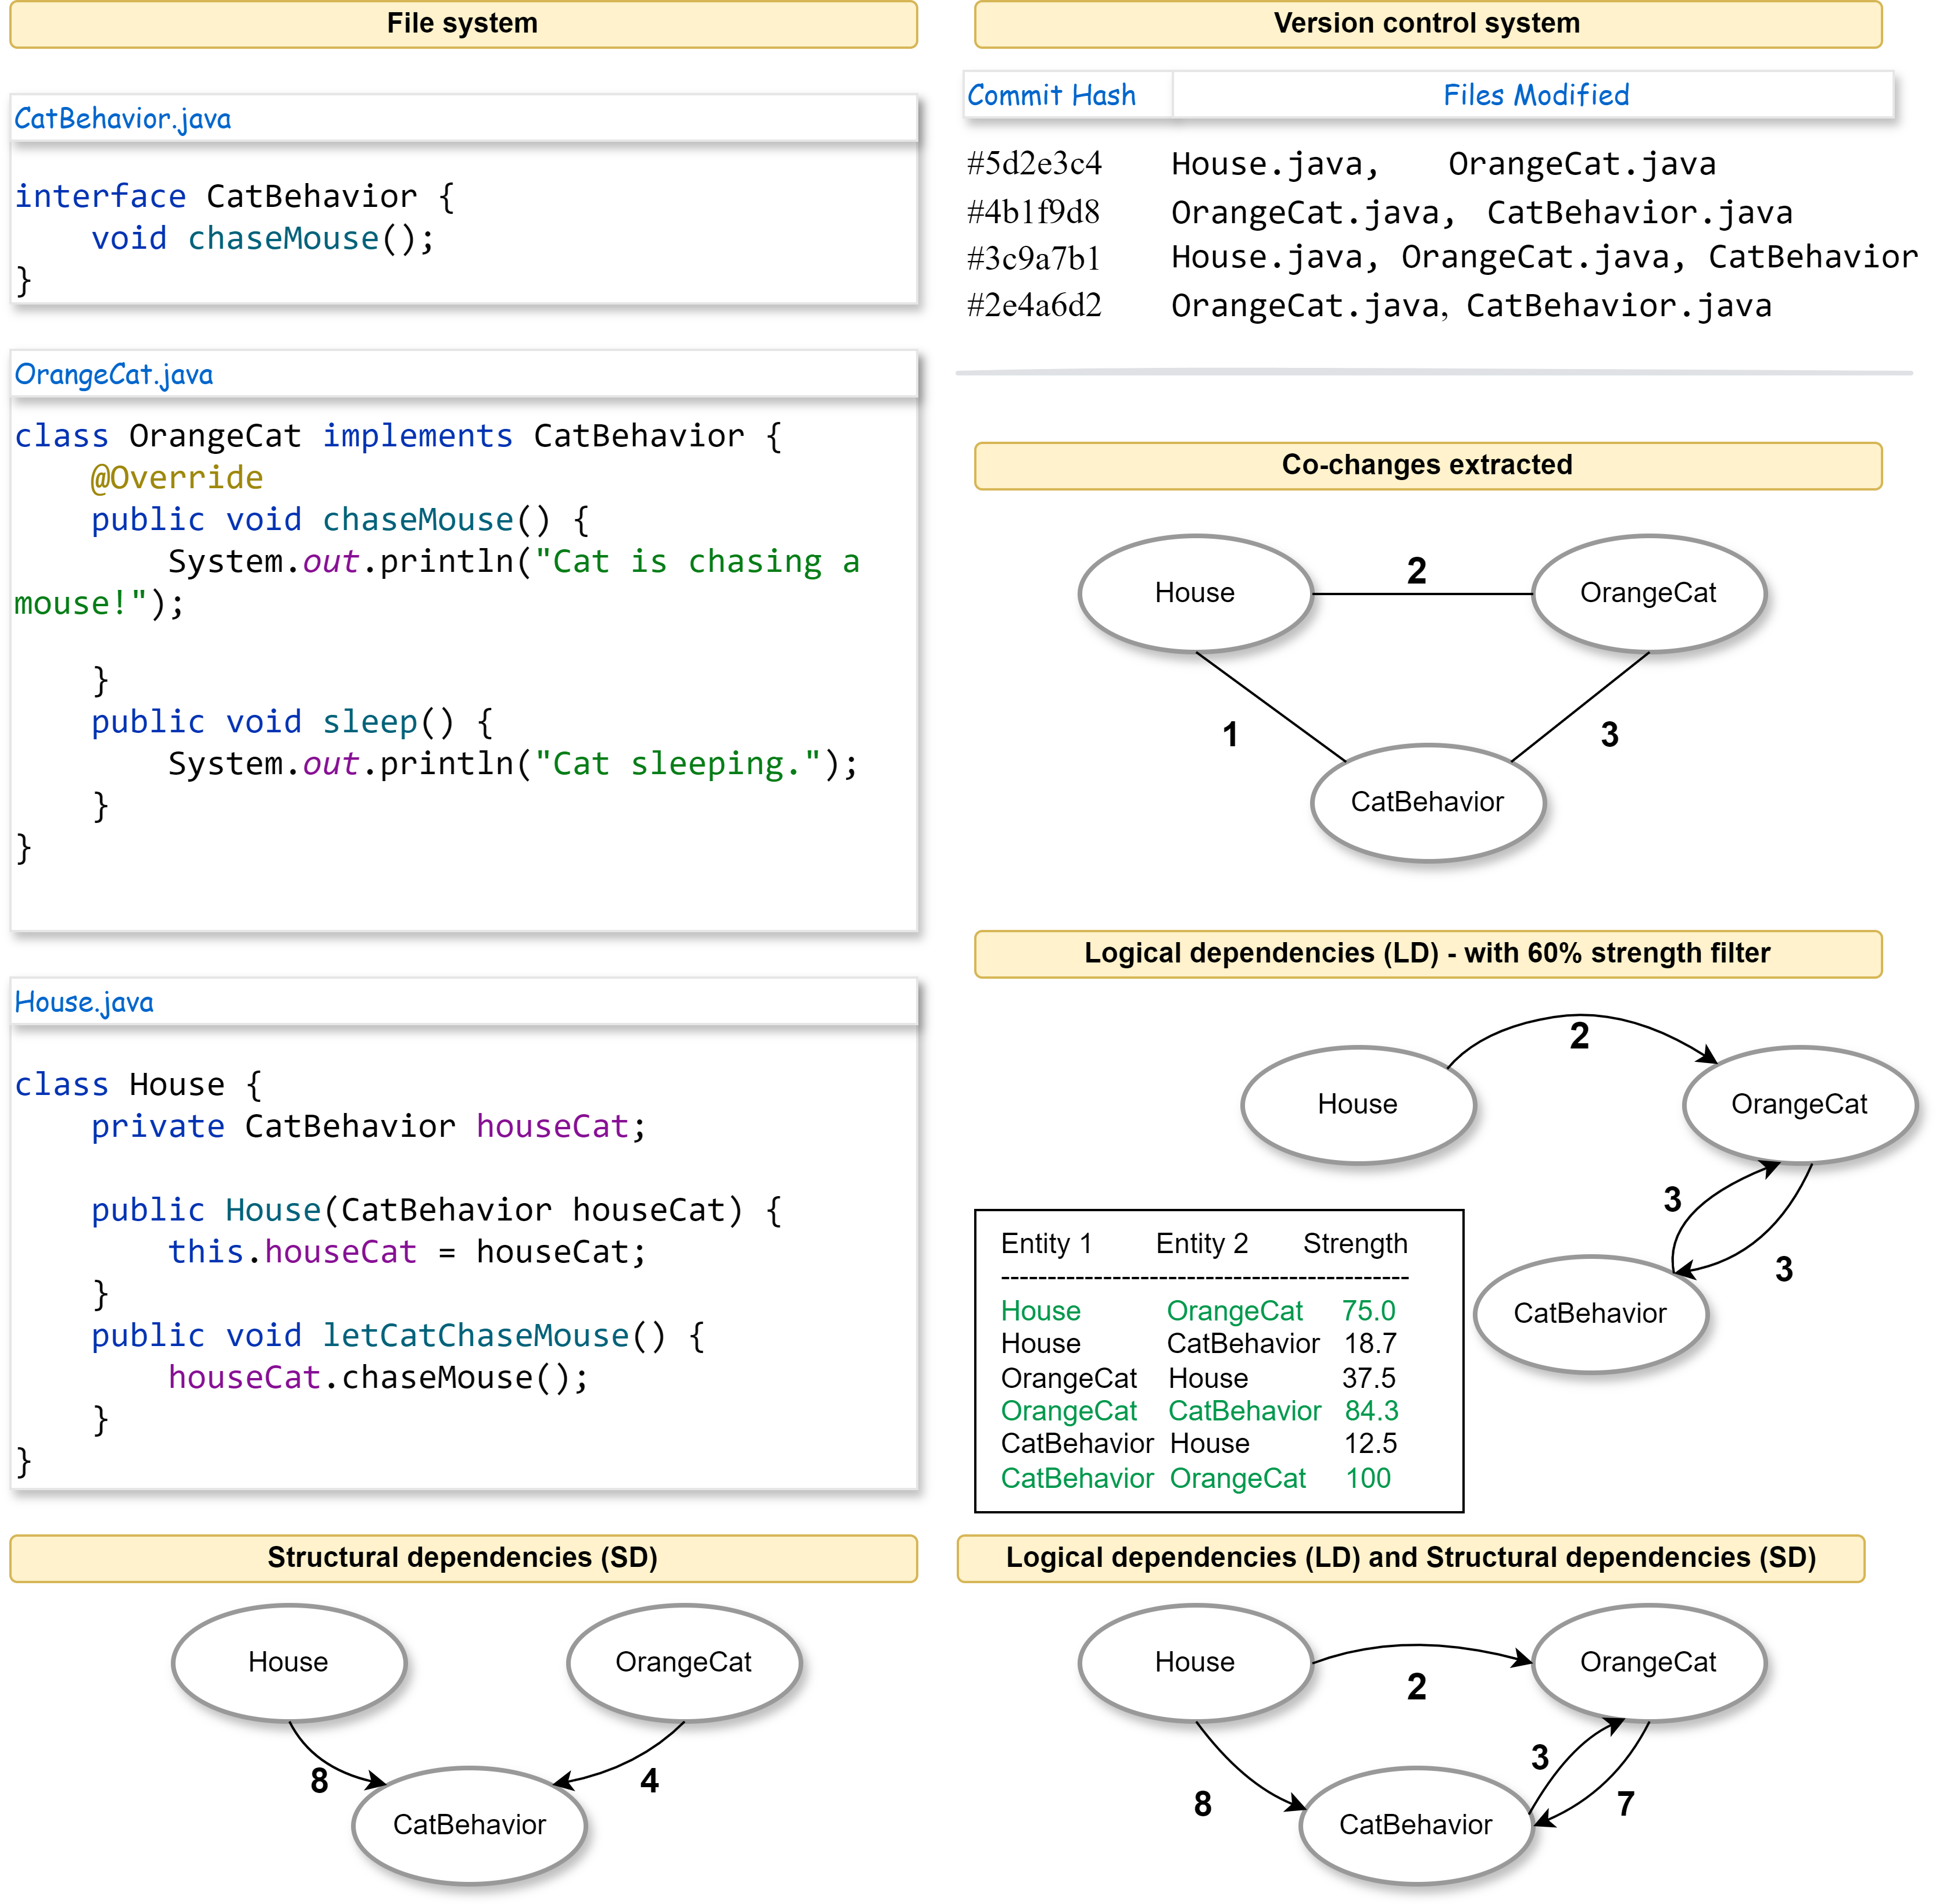
\includegraphics[width=\columnwidth]{codegraph.png}
  \caption{Dependency Graph: Combining structural and logical dependencies.}
  \label{fig:codegraph}
\end{figure}

When structural dependencies (SD) and logical dependencies (LD) are combined in software clustering, both types of relationships are represented within the same graph.

Each entity in the system is represented as a node in the graph, and the dependencies between them are represented as directed weighted edges.

\textit{SD and LD weights are combined} when the same pair of entities appear in both dependencies. In this case, the weights from SD and LD are summed, giving more influence to those entity pairs. When a pair of entities appear only in SD or only in LD, the edge is added to the graph together with its corresponding weight.

Figure \ref{fig:codegraph} illustrates combining structural and logical dependencies in the same dependency graph. The structural dependencies between \texttt{House}, \texttt{OrangeCat}, and \texttt{CatBehavior} entities are visible from the source code analysis.

However, the combination of SD and LD reveals additional insights. One important observation is the logical dependency between \texttt{House} and \texttt{OrangeCat}, which is not observed from the structural analysis. This relation is extracted from version control and filtered using a 60\% strength filter. The strength metric reveals that \texttt{House} and \texttt{OrangeCat} have a significant co-change value of 75.0, usually associated with a strong relationship.

When SD and LD overlap, such as between \texttt{OrangeCat} and \texttt{CatBehavior}, their weights are summed. This summation increases the weight of the dependency, making it more important in the dependency graph.



\chapter{Logical dependencies in key class detection}
\label{cap:usage}

\section{Introduction}
\label{sec:introduction}
Zaidman et al \cite{ZaidmanJurnal} were the first to introduce the concept of key classes and it refers to classes that can be found in documents written to provide an architectural overview of the system or an introduction to the system structure. 
Tahvildari and Kontogiannis have a more detailed definition regarding key classes concept: “Usually, the most important concepts of a system are implemented by very few key classes which can be characterized by the specific properties. These classes, which we refer to as key classes, manage many other classes or use them in order to implement their functionality. The key classes are tightly coupled with other parts of the system. Additionally, they tend to be rather complex, since they implement much of the legacy system’s functionality” \cite{Tahvildari2004ImprovingDQ}.
Also, other researchers use a similar concept as the one defined by Zaidman but under different terms like important classes  \cite{Meyer2014IdentifyingIC} or central software classes \cite{CentralClassesSteidl}.


The key class identification can be done by using different algorithms with different inputs. In the research of Osman et al., the key class identification is made by using a machine learning algorithm and class diagrams as input for the algorithm \cite{6676885}. Thung et al. builds on top of Osman et al.’s approach and adds network metrics and optimistic classification in order to detect key classes \cite{rocclasification}.  

Zaidman et al. use a webmining algorithm and dynamic analysis of the source code to identify the key classes \cite{ZaidmanJurnal}.

Sora et al. use a page ranking algorithm for finding key classes and static analysis of the source code \cite{PagerankENASE}, \cite{enase15}, \cite{SoraSpringer}, \cite{PagerankSACI}. In \cite{Finding-key-classes} the authors use in addition to the previous research also other class attributes to identify important classes.
The page ranking algorithm is a customization of PageRank, the algorithm used to rank web pages \cite{ilprints422}.
The PageRank algorithm works based on a recommendation system. If one node has a connection with another node, then it recommends the second node. In previous works, connections are established based on structural dependencies extracted from static code analysis. If A has a structural dependency with B, then A recommends B, and also B recommends A.

The ranking algorithm ranks all the classes from the source code of the system analyzed according to their importance. To identify the important classes from the rest of the classes a threshold for TOP classes from the top of the ranking is set. The TOP threshold value can go from 1 to the total number of classes found in the system. 

Some researchers \cite{ZaidmanJurnal}, \cite{Ding2016AnIA}, \cite{PAN2018188} consider that 15\% of the total number of classes of the system is a suited value for the TOP threshold. Other researchers \cite{Finding-key-classes} consider that 15\% of the total number of classes is a too high value for the TOP threshold and suggest that a value in the range of 20–30 is better.


\section{Metrics for results evaluation}
\label{sec:evalmetrics}
To evaluate the quality of the key classes ranking algorithm and solution produced, the key classes found by the algorithm are compared with a reference solution.

The reference solution is extracted from the developer documentation.  Classes mentioned in the documentation are considered key classes and form the reference solution (ground truth) used for validation \cite{7551990}. 


For the comparison between both solutions, is used a classification model. The quality of the solution produced is evaluated by using metrics that evaluate the performance of the classification model, such as Precision-Recall and Receiver Operating Characteristic Area Under Curve (ROC-AUC).

A classification model (or "classifier") is a mapping between expected results and predicted results \cite{ROCIntro}, \cite{ROCBRADLEY19971145}. Both results can be labeled as positive or negative, which leads us to the confusion matrix from figure \ref{fig:confusion}. 
\begin{figure}[h]
\centering
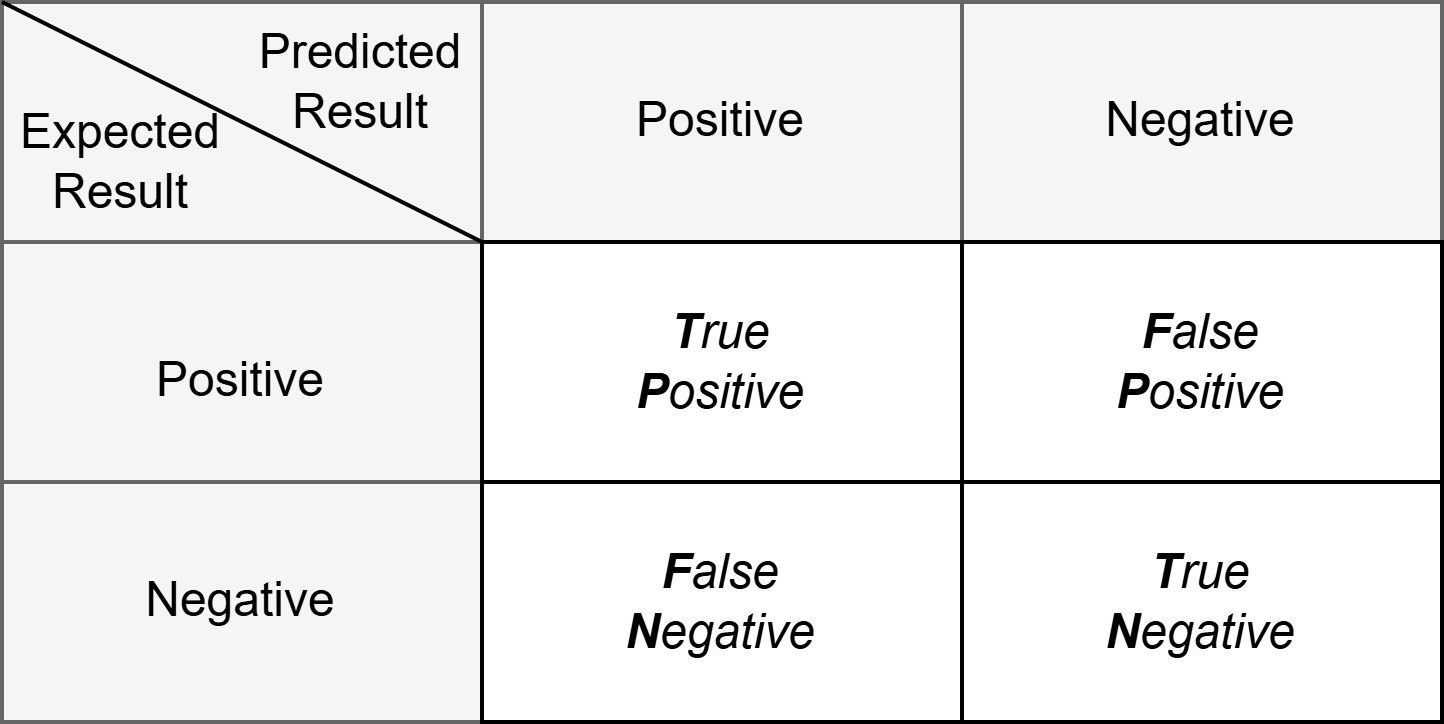
\includegraphics[scale=0.9]{confusion.png}
\caption{Confusion matrix}
\label{fig:confusion}
\centering
\end{figure}
The confusion matrix has the following outcomes:
		\begin{itemize}
			\item \textit{true positive}, if the expected result is positive and the predicted result is also positive.
			\item \textit{false positive}, if the expected result is positive but the predicted result is negative.
			\item \textit{false negative}, if the expected result is negative but the predicted result is positive.
			\item \textit{true negative}, if the expected result is negative and the predicted result is also negative.
		\end{itemize}


\textit{Precision-recall}


Precision is the ratio of True Positives to all the positives of the result set.

\begin{equation}
 precision = \frac{TP}{TP+FN}
\end{equation}
The recall is the ratio of True Positives to all the positives of the reference set.

\begin{equation}
 recall = \frac{TP}{TP+FP}
\end{equation}

As mentioned in section \ref{sec:introduction}, to distinguish the key classes from the rest of the classes a TOP threshold is used. Some researchers consider that 15\% of the total classes is the best value for the TOP threshold and others consider that the value should be in the range of 20-30. 

The precision-recall metric is suited if the threshold value is fixed. If the threshold value is variable, then metrics that capture the behavior over all possible values must be used. Such metric is the Receiver Operating Characteristic metric.

\textit{Receiver Operating Characteristic Area Under Curve}


The ROC graph is a two-dimensional graph that has on the X-axis plotted the false positive rate and on the Y-axis the true positive rate. By plotting the true positive rate and the false positive rate at thresholds that vary between a minimum and a maximum possible value we obtain the ROC curve. The area under the ROC curve is called Area Under the Curve (AUC).

The true positive rate of a classifier is calculated as the division between the number of true positive results identified and all the positive results identified:

\begin{equation}
 True\ positive\ rate (TPR) = \frac{TP}{TP+FN}
\end{equation}
The false positive rate of a classifier is calculated as the division between the number of false positive results identified and all the negative results identified:

\begin{equation}
 False\ positive\ rate (FPR) = \frac{FP}{FP+TN}
\end{equation}


In multiple related works, the ROC-AUC metric has been used to evaluate the results for finding key classes of software systems.
For a classifier to be considered good, its ROC-AUC metric value should be as close to 1 as possible, when the value is 1 then the classifier is considered to be perfect.

Osman et al. obtained in their research an average Area Under the Receiver Operating Characteristic Curve (ROC-AUC) score of 0.750 \cite{6676885}. Thung et al. obtained an average ROC-AUC score of 0.825 \cite{rocclasification}  and Sora et al. obtained an average ROC-AUC score of 0.894 \cite{Finding-key-classes}.


\section{Data set used}
\label{sec:dataset}
In this section, we will look over all the systems studied in the baseline research presented in section \ref{sec:previous_measurements}, and we will try to identify the systems that could be used also in our current research involving logical dependencies.


The research of I. Sora et al \cite{Finding-key-classes} takes into consideration structural public dependencies that are extracted using static analysis techniques and was performed on the object-oriented systems presented in table \ref{tab:keyclass:overview}.

The requirements for a system to qualify as suited for investigations using logical dependencies are: has to be on GitHub, has to have release tags to identify the version, and also has to have an increased number of commits. 
From the total of 14 object-oriented systems listed in the paper \cite{Finding-key-classes}, 13 of them have repositories in Github \ref{tab:gitfoundsystems}. And from the found repositories we identified only 6 repositories that have the same release tag as the specified version from table \ref{tab:keyclass:overview}. It is important to identify the correct release tag for each repository to limit the commits further analyzed by date. Only commits that were made until the specified release are considered and analyzed.
The commits number found on the remaining 6 repositories varies from 19108 commits for Tomcat Catalina to 149 commits for JHotDraw. In order to have more accurate results, we need a significant number of commits, so we reached the conclusion that only 3 systems can be used for key classes detection using logical dependencies: Apache Ant, Hibernate, and Tomcat Catalina.  From all the systems mentioned in table \ref{tab:keyclass:overview} Apache Ant is the most used and analyzed in other  works \cite{enase19}, \cite{7332515}, \cite{1402122}, \cite{Kamran2016IdentificationOC}.

\begin{table}[H]
\renewcommand{\arraystretch}{1}
\caption{Analyzed software systems in previous research paper.}
\label{tab:keyclass:overview}
\centering
\resizebox{\textwidth}{!}{
\begin{tabular}{|c|c|p{7cm}|c|}
\hline
ID	&	System	&	Description	&	Version	\\
\hline
Sl	&	Apache Ant	&	Java library and command line tool that drive the build processes as targets and extension points depending upon each other	&	1.6.1	\\ \hline
S2	&	Argo UML	&	UML modelling tool with support for all UML diagrams.	&	0.9.5	\\ \hline
S3	&	GWT Portlets	&	Open source web framework for building GWT (Google Web Toolkit) Applications.	&	0.9.5 beta	\\ \hline
S4	&	Hibernate 	&	Persistence framework for Java.	&	5.2.12	\\ \hline
S5	&	javaclient	&	Java distributed application for playing with robots	&	2.0.0	\\ \hline
S6	&	jEdit	&	Java mature text editor for programmers.	&	5.1.0	\\ \hline
S7	&	JGAP	&	Genetic Algorithms and Genetic Programming Java library.	&	3.6.3	\\ \hline
S8	&	JHotDraw	&	JHotDraw is a two-dimensional graphics framework for structured drawing editors that is written in Java.	&	6.0b.1	\\ \hline
S9	&	JMeter	&	JMeter is a Java application designed to load test functional behavior and measure performance	&	2.0.1	\\ \hline
S10	&	Log4j	&	Logging Service	&	2.10.0	\\ \hline
S11	&	Mars	&	The Mars Simulation Project is a Java project that models and simulates human settlements on Mars planet	&	3.06.0	\\ \hline
S12	&	Maze	&	The Maze-solver project simulates an artificial intelligence algorithm on a maze	&	1.0.0	\\ \hline
S13	&	Neuroph	&	Neuroph is a Java neural network framework.	&	2.2.0	\\ \hline
S14	&	Tomcat Catalina	&	The Apache Tomcat project is an open-source implementation of JavaServlet and JavaServerPages technologies	&	9.0.4	\\ \hline
S15	&	Wro4J	&	The Wro4J is a web resource (JS and CSS) optimizer for Java.	&	1.6.3	\\ 
\hline
\end{tabular}
}
\end{table}



\begin{table}[H]
\renewcommand{\arraystretch}{1}
\caption{Found systems and versions of the systems in GitHub. }
\label{tab:gitfoundsystems}
\centering
\scalebox{0.8}{
\begin{tabular}{|c|c|c|c|c|}
\hline
ID	&	System	&	Version	&	Release Tag name	&	Commits number	\\
\hline
\rowcolor{lightgreen}
Sl	&	Apache Ant	&	1.6.1	&	rel/1.6.1	&	6713	\\
S2	&	Argo UML	&	0.9.5	&	not found	&	0	\\
S3	&	GWT Portlets	&	0.9.5 beta	&	not found	&	0	\\
\rowcolor{lightgreen}
S4	&	Hibernate 	&	5.2.12	&	5.2.12	&	6733	\\
S5	&	javaclient	&	2.0.0	&	not found	&	0	\\
S6	&	jEdit	&	5.1.0	&	not found	&	0	\\
S7	&	JGAP	&	3.6.3	&	not found	&	0	\\
S8	&	JHotDraw	&	6.0b.1	&	not found	&	149	\\
S9	&	JMeter	&	2.0.1	&	v2\_1\_1	&	2506	\\
S10	&	Log4j	&	2.10.0	&	v1\_2\_10-recalled	&	634	\\
S11	&	Mars	&	3.06.0	&	not found	&	0	\\
S12	&	Maze	&	1.0.0	&	not found	&	0	\\
S13	&	Neuroph	&	2.2.0	&	not found	&	0	\\
\rowcolor{lightgreen}
S14	&	Tomcat Catalina	&	9.0.4	&	9.0.4	&	19108	\\
S15	&	Wro4J	&	1.6.3	&	v1.6.3	&	2871	\\
\hline
\end{tabular}
}
\end{table}



\section{Measurements using logical dependencies}
\label{sec:current_measurements}

As we mentioned in the beginning the purpose is to check if the logical dependencies can improve key class detection. 

As presented in section \ref{sec:previous_measurements}, and section \ref{sec:introduction} the key class detection was done by using structural dependencies of the system. 
In this section, we will use the same tool used in the baseline approach presented in section \ref{sec:previous_measurements}, and we will add a new input to it, the logical dependencies. 

Below is a comparison between the new approach and baseline approach, how we collect the logical dependencies, the results obtained previously, and the new results obtained. 
The new results are separated into two categories, the results obtained by using structural and logical dependencies and the results obtained by using only logical dependencies. 


\subsection{Baseline approach}
\label{sec:previous_measurements}

We use the research of I. Sora et al \cite{Finding-key-classes} as a baseline for our research involving the usage of logical dependencies to find key classes. 
The baseline approach uses a tool that takes as an input the source code of the system and applies ranking strategies to rank the classes according to their importance. 

In order to rank the classes according to their importance, different class metrics are used \cite{Ding2016AnIA}, \cite{ZaidmanJurnal}, \cite{PAN2018188}. Below are presented some of the class metrics used in the baseline approach in order to rank the classes according to their importance.



\subsubsection{Class attributes that characterize key classes}
The metrics used in the baseline research can be grouped into the following categories: 

\begin{itemize}
	\item class size metrics: number of fields (NoF),  number of methods (NoM), global size (Size = NoF+NoM).
	\item class connection metrics, any structural dependency between two classes:
		\begin{itemize}
			\item CONN-IN, the number of distinct classes that use a class;
			\item CONN-OUT, the total number of distinct classes that are used by a class;
			\item CONN-TOTAL, the total number of distinct classes that a class uses or are used by a class (CONN-IN + CONN-OUT).
			\item CONN-IN-W, the total weight of distinct classes that use a class. 
			\item CONN-OUT-W, the total weight of distinct classes that are used by a class. 
			\item CONN-TOTAL-W, the total weight of all connections of the class (CONN-IN-W + CONN-OUT-W) \cite{Finding-key-classes}.
		\end{itemize}
	\item class pagerank values, previous research use pagerank values computed on both directed and undirected, weighted and unweighted graphs:
		\begin{itemize}
			\item PR - value computed on the directed and unweighted graph;
			\item PR-W - value computed on the directed and weighted graph;
			\item PR-U - value computed on the undirected and unweighted graph;
			\item PR-U-W - value computed on the undirected and weighted graph;
			\item PR-U2-W - value computed on the weighted graph with back-recommendations \cite{PagerankENASE}, \cite{enase15}, \cite{Finding-key-classes}, \cite{PagerankSACI}.
		\end{itemize}
\end{itemize}


Based on the class attributes presented, all the classes of the system are ranked. To differentiate the important (key) classes from the rest of the classes, a TOP threshold for the top classes found is set. 
The threshold vary between 20 and 30 classes.



The baseline approach not only identifies the key classes but also evaluates the performance of the solution produced. 
The same approach as the one presented in section \ref{sec:evalmetrics} is used for the evaluation of the results. The key classes found by the ranking algorithm are compared with a reference solution that is extracted from the developer documentation by using a classification model.

The true positives (TP) are the classes found in the reference solution and also in the top TOP ranked classes. False positives (FP) are the classes that are not in the reference solution but are in the TOP ranked classes.
True Negatives (TN) are classes that are found neither in the reference solution nor in the TOP ranked classes. False Negatives (FN) are classes that are found in the reference solution but not found in the TOP ranked classes.


Due to the fact that the TOP threshold is varied, the Receiver Operating Characteristic Area Under Curve metric is used for the evaluation of the results.

The entire workflow of the baseline approach that was presented above is also presented in figure \ref{fig:baseline_approach}.

\begin{figure}[H]
\centering
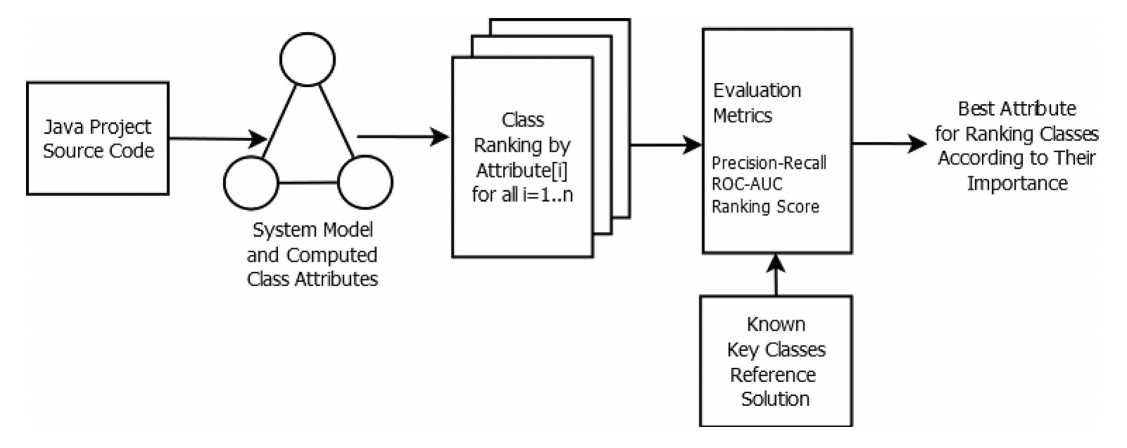
\includegraphics[width=\textwidth]{baseline_approach.PNG}
\caption{Overview of the baseline approach. Reprinted from “Finding key classes in object-oriented
software systems by techniques based on static analysis.” by Ioana Sora and Ciprian-Bogdan Chirila, 2019, Information and Software Technology, 116:106176. Reprinted with permission. }
\label{fig:baseline_approach}
\centering
\end{figure}




\subsection{Comparison with the baseline approach}
\label{sec:comparison}

The baseline approach uses a tool that takes as input the source code of the system to identify the key classes and the reference solution to evaluate the quality of the solution. 
We modified the tool such that it can also take as input the logical dependencies. 

In order to rank the classes according to their importance, the tool uses different class metrics. The list of the metrics used in the baseline approach is presented in section \ref{sec:previous_measurements}.  
The difference in the metrics used compared with the baseline approach is that we use a subset of those metrics. The reason why we are not using all the metrics is that the extracted logical dependencies are undirected. The metrics used by the current approach are CONN-TOTAL, CONN-TOTAL-W, PR-U, PR-U-W, and PR-U2-W.

We did not change the rest of the workflow of the tool. Meaning that the TOP threshold is varied between 20 and 30 and the resulting solution is evaluated by using the ROC-AUC metric. The goal being a ROC-AUC (Receiver Operating Characteristic - Area Under the Curve) metric value as close to 1 as possible.

\begin{figure}[H]
\centering
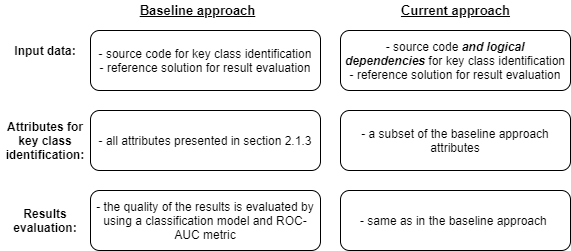
\includegraphics[width=\textwidth]{baseline_comparison.png}
\caption{ Comparison between the new approach and the baseline }
\label{fig:baseline_comparison}
\centering
\end{figure}

\subsection{Logical dependencies collection and current workflow used}

The logical dependencies are those co-changing pairs extracted from the versioning system history that remain after filtering. The filtering part consists of applying two filters: the filter based on commit size and the filter based on connection strength. 

To determine the connection strength of a pair, we first need to calculate the connection factors for both entities that form a co-changing pair.
Assuming that we have a co-changing pair formed by entities A and B, the connection factor of entity A with entity B is the percentage from the total commits involving A that contains entity B. The connection factor of entity B with entity A is the percentage from the total commits involving B that contain also entity A.

\begin{equation}
 connection\ factor\ for\ A = \frac{100 * commits\ involving\ A\ and\ B}{total\ nr\ of\ commits\ involving\ A}
\end{equation}

\begin{equation}
 connection\ factor\ for\ B = \frac{100 * commits\ involving\ A\ and\ B}{total\ nr\ of\ commits\ involving\ B}
\end{equation}

We calculated the connection factor for each entity involved in a co-changing pair and filtered the co-changing pairs based on it. The rule set is that both entities had to have a connection factor with each other greater than the threshold value.

After the filtering part, the remaining co-changing pairs, now called logical dependencies, are exported in CSV files.

The entire process of extracting co-changing pairs from the versioning system, filter them, and export the remaining ones into CSV files is done with a tool written in Python.

The next step is to use the exported logical dependencies for key classes detection. In order to do that we used the same key class detection tool used in the previous research presented in section \ref{sec:previous_measurements}. We adapted the tool to be able to process also logical dependencies because previously the tool used only structural dependencies extracted from the source code of the software systems. 
The workflow is presented in figure \ref{fig:workflow_key}

\begin{figure}[H]
\centering
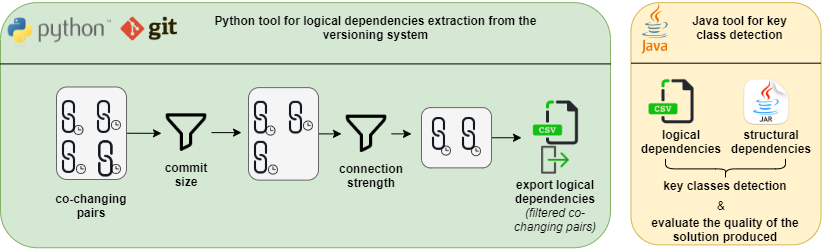
\includegraphics[width=\textwidth]{key_class_workflow.png}
\caption{Workflow for key classes detection}
\label{fig:workflow_key}
\centering
\end{figure}


\subsection{Measurements using only the baseline approach}


In table \ref{tab:previousresults} are presented the ROC-AUC values for different attributes computed for the systems Ant, Tomcat Catalina, and Hibernate by using the baseline approach. We intend to compare these values with the new values obtained by using also logical dependencies in key class detection.

\begin{table}[!h]
\renewcommand{\arraystretch}{1}
\caption{ROC-AUC metric values extracted. }
\label{tab:previousresults}
\centering
\scalebox{0.9}{
\begin{tabular}{|c|ccc|}
\hline
Metrics &	Ant	&	Tomcat Catalina	&	Hibernate	\\
\hline

PR\_U2\_W	&	0.95823	&	0.92341	&	0.95823	\\
PR	&	0.94944	&	0.92670	&	0.94944	\\
PR\_U	&	0.95060	&	0.93220	&	0.95060	\\
CONN\_TOTAL\_W	&	0.94437	&	0.92595	&	0.94437	\\
CONN\_TOTAL	&	0.94630	&	0.93903	&	0.94630	\\

\hline
\end{tabular}
}
\end{table}





\subsection{Measurements using combined structural and logical dependencies}

The tool used in the baseline approach runs a graph-ranking algorithm. 
The graph used contains the structural dependencies extracted from static source code analysis.
Each edge in the graph represents a dependency, the entities that form a structural dependency are represented as vertices in the graph. 
As mentioned in section \ref{sec:comparison}, we modified the tool to read also logical dependencies and add them to the graph. 
In this section, we add in the graph the logical dependencies together with the structural dependencies. 

In tables \ref{tab:measurementscombined:ant}, \ref{tab:measurementscombined:tomcat}, and \ref{tab:measurementscombined:hibernate}, on each line, we have the metric that is calculated and on each column, we have the connection strength threshold that was applied to the logical dependencies used in identifying the key classes.
We started with logical dependencies that have a connection strength greater than 10\%, which means that in at least 10\% of the commits involving A or B, A and B update together. Then we increased the threshold value by 10 until we remained only with entities that update in all the commits together. The last column contains the results obtained previously by the tool by only using structural dependencies.

As for the new results obtained by combining structural and logical dependencies, highlighted with orange are the values that are close to the previously registered values but did not surpass them. Highlighted with green are values that are better than the previously registered values. At this step, we can also observe that for all three systems measured in tables \ref{tab:measurementscombined:ant}, \ref{tab:measurementscombined:tomcat}, and \ref{tab:measurementscombined:hibernate}, the best values obtained are for connection strength between 40-70\%.

\begin{table}[!h]
\renewcommand{\arraystretch}{1}
\caption{Measurements for Ant using structural and logical dependencies combined}
\label{tab:measurementscombined:ant}
\centering
\scalebox{0.7}{
\begin{tabular}{|c|cccccccccc|c|}
\hline
Metrics &	$\geq10\%$	&	$\geq20\%$		&	$\geq30\%$		&	$\geq40\%$		&	$\geq50\%$		&	$\geq60\%$		&	$\geq70\%$		&	$\geq80\%$		&	$\geq90\%$		&	$\geq100\%$		&	Baseline \\
\hline

PR\_U2\_W	&	0.924	&	0.925	&	0.926	&	0.927	&	0.927	&	0.927	&	\cellcolor{lightgreen}0.929	&	0.928	&	0.928	&	0.928	&	0.929	\\
PR	&	0.914	&	0.854	&	0.851	&	\cellcolor{lightgreen}0.866	&	\cellcolor{lightgreen}0.876	&	\cellcolor{lightgreen}0.882	&	\cellcolor{lightgreen}0.887	&	0.854	&	0.852	&	0.852	&	0.855	\\
PR\_U	&	0.910	&	0.930	&	0.933	&	0.933	&	\cellcolor{lightgreen}0.935	&	\cellcolor{lightgreen}0.934	&	\cellcolor{lightgreen}0.939	&	0.933	&	0.933	&	0.933	&	0.933	\\
CON\_T\_W	&	0.924	&	0.928	&	0.931	&	0.932	&	0.933	&	0.934	&	\cellcolor{lightgreen}0.936	&	0.934	&	0.934	&	0.934	&	0.934	\\
CON\_T	&	0.840	&	0.886	&	0.904	&	0.909	&	0.915	&	0.923	&	0.932	&	0.935	&	\cellcolor{lightorange}0.936	&	\cellcolor{lightorange}0.936	&	0.942	\\

\hline
\end{tabular}
}
\end{table}


\begin{table}[!h]
\renewcommand{\arraystretch}{1}
\caption{Measurements for Tomcat using structural and logical dependencies combined}
\label{tab:measurementscombined:tomcat}
\centering
\scalebox{0.7}{
\begin{tabular}{|c|cccccccccc|c|}
\hline
Metrics &	$\geq10\%$	&	$\geq20\%$		&	$\geq30\%$		&	$\geq40\%$		&	$\geq50\%$		&	$\geq60\%$		&	$\geq70\%$		&	$\geq80\%$		&	$\geq90\%$		&	$\geq100\%$		&	Baseline \\
\hline

PR\_U2\_W	&	0.910	&	0.917	&	0.923	&	\cellcolor{lightgreen}0.924	&	\cellcolor{lightgreen}0.924	&	\cellcolor{lightgreen}0.924	&	\cellcolor{lightgreen}0.924	&	\cellcolor{lightgreen}0.924	&	\cellcolor{lightgreen}0.924	&	\cellcolor{lightgreen}0.924	&	0.923	\\
PR	&	0.811	&	0.800	&	0.815	&	0.834	&	0.847	&	0.852	&	0.853	&	0.858	&	0.858	&	0.858	&	0.927	\\
PR\_U	&	0.910	&	0.921	&	0.931	&	\cellcolor{lightgreen}0.933	&	\cellcolor{lightgreen}0.933	&	0.932	&	\cellcolor{lightgreen}0.933	&	0.932	&	0.932	&	0.932	&	0.932	\\
CON\_T\_W	&	0.914	&	0.920	&	0.924	&	\cellcolor{lightorange}0.926	&	0.926	&	0.926	&	0.926	&	0.926	&	0.926	&	0.926	&	0.926	\\
CON\_T	&	0.868	&	0.906	&	0.930	&	0.936	&	0.937	&	\cellcolor{lightorange}0.938	&	0.938	&	0.938	&	0.938	&	0.938	&	0.939	\\
																												

\hline
\end{tabular}
}
\end{table}


\begin{table}[!h]
\renewcommand{\arraystretch}{1}
\caption{Measurements for Hibernate using structural and logical dependencies combined}
\label{tab:measurementscombined:hibernate}
\centering
\scalebox{0.7}{
\begin{tabular}{|c|cccccccccc|c|}
\hline
Metrics &	$\geq10\%$	&	$\geq20\%$		&	$\geq30\%$		&	$\geq40\%$		&	$\geq50\%$		&	$\geq60\%$		&	$\geq70\%$		&	$\geq80\%$		&	$\geq90\%$		&	$\geq100\%$		&	Baseline \\
\hline

PR\_U2\_W	&	0.954	&	0.957	&	\cellcolor{lightorange}0.958	&	0.958	&	0.958	&	0.958	&	0.958	&	0.958	&	0.958	&	0.958	&	0.958	\\
PR	&	0.929	&	0.929	&	0.933	&	0.939	&	0.939	&	0.946	&	\cellcolor{lightorange}0.947	&	0.947	&	0.947	&	0.947	&	0.949	\\
PR\_U	&	0.942	&	0.947	&	0.948	&	0.949	&	0.949	&	\cellcolor{lightorange}0.950	&	0.950	&	0.950	&	0.950	&	0.950	&	0.951	\\
CON\_T\_W	&	0.939	&	0.942	&	0.943	&	0.944	&	0.944	&	\cellcolor{lightgreen}0.945	&	\cellcolor{lightgreen}0.945	&	\cellcolor{lightgreen}0.945	&	\cellcolor{lightgreen}0.945	&	\cellcolor{lightgreen}0.945	&	0.944	\\
CON\_T	&	0.924	&	0.933	&	0.938	&	0.941	&	0.941	&	0.944	&	\cellcolor{lightorange}0.945	&	0.945	&	0.945	&	0.945	&	0.946	\\


\hline
\end{tabular}
}
\end{table}





\subsection{Measurements using only logical dependencies}
In the previous section, we added in the graph based on which the ranking algorithm works the logical and structural dependencies. In the current section, we will add only the logical dependencies to the graph.

In tables \ref{tab:measurementshistory:ant}, \ref{tab:measurementshistory:tomcat}, and \ref{tab:measurementshistory:hibernate}, are presented the results obtained by using only logical dependencies to detect key classes. The measurements obtained are not as good as using logical and structural dependencies combined or using only structural dependencies. But, all the values obtained are above 0.5, which means that a good part of the key classes is detected by only using logical dependencies.  As mentioned in section \ref{sec:evalmetrics}, a classifier is good if it has the ROC-AUC value as close to 1 as possible. 


One possible explanation for the less performing results is that the key classes may have a better design than the rest of the classes, which means that are less prone to change. If the key classes are less prone to change, this implies that the number of dependencies extracted from the versioning system can be less than for other classes.

\begin{table}[!h]
\renewcommand{\arraystretch}{1}
\caption{Measurements for Ant using only logical dependencies}
\label{tab:measurementshistory:ant}
\centering
\scalebox{0.7}{
\begin{tabular}{|c|cccccccccc|c|}
\hline
Metrics &	$\geq10\%$	&	$\geq20\%$		&	$\geq30\%$		&	$\geq40\%$		&	$\geq50\%$		&	$\geq60\%$		&	$\geq70\%$		&	$\geq80\%$		&	$\geq90\%$		&	$\geq100\%$		&	Baseline \\
\hline

PR\_U2\_W	&	0.720	&	0.627	&	0.718	&	0.703	&	0.732	&	0.824	&	0.852	&	\cellcolor{lightorange}0.881	&	0.876	&	0.876	&	0.929	\\
PR	&	0.720	&	0.627	&	0.718	&	0.703	&	0.732	&	0.824	&	0.852	&	\cellcolor{lightorange}0.881	&	0.876	&	0.876	&	0.855	\\
PR\_U	&	0.720	&	0.627	&	0.718	&	0.703	&	0.732	&	0.824	&	0.852	&	\cellcolor{lightorange}0.881	&	0.876	&	0.876	&	0.933	\\
CON\_T\_W	&	0.722	&	0.581	&	0.644	&	0.676	&	0.727	&	0.819	&	0.842	&	0.874	&	\cellcolor{lightorange}0.876	&	0.876	&	0.934	\\
CON\_T	&	0.722	&	0.581	&	0.644	&	0.676	&	0.727	&	0.819	&	0.842	&	0.874	&	\cellcolor{lightorange}0.876	&	0.876	&	0.942	\\

\hline
\end{tabular}
}
\end{table}


\begin{table}[!h]
\renewcommand{\arraystretch}{1}
\caption{Measurements for Tomcat using only logical dependencies}
\label{tab:measurementshistory:tomcat}
\centering
\scalebox{0.7}{
\begin{tabular}{|c|cccccccccc|c|}
\hline
Metrics &	$\geq10\%$	&	$\geq20\%$		&	$\geq30\%$		&	$\geq40\%$		&	$\geq50\%$		&	$\geq60\%$		&	$\geq70\%$		&	$\geq80\%$		&	$\geq90\%$		&	$\geq100\%$		&	Previous \\
\hline

PR\_U2\_W	&	0.672	&	0.656	&	0.645	&	0.697	&	0.754	&	0.776	&	0.786	&	\cellcolor{lightorange}0.799	&	0.799	&	0.799	&	0.923	\\
PR	&	0.685	&	0.643	&	0.642	&	0.697	&	0.754	&	0.776	&	0.786	&	\cellcolor{lightorange}0.799	&	0.799	&	0.799	&	0.927	\\
PR\_U	&	0.685	&	0.643	&	0.644	&	0.697	&	0.754	&	0.776	&	0.786	&	\cellcolor{lightorange}0.799	&	0.799	&	0.799	&	0.932	\\
CON\_T\_W	&	0.694	&	0.636	&	0.636	&	0.697	&	0.754	&	0.776	&	0.786	&	\cellcolor{lightorange}0.799	&	0.799	&	0.799	&	0.926	\\
CON\_T	&	0.654	&	0.611	&	0.636	&	0.697	&	0.754	&	0.776	&	0.786	&	\cellcolor{lightorange}0.799	&	0.799	&	0.799	&	0.939	\\

				
\hline
\end{tabular}
}
\end{table}


\begin{table}[!h]
\renewcommand{\arraystretch}{1}
\caption{Measurements for Hibernate using only logical dependencies}
\label{tab:measurementshistory:hibernate}
\centering
\scalebox{0.7}{
\begin{tabular}{|c|cccccccccc|c|}
\hline
Metrics &	$\geq10\%$	&	$\geq20\%$		&	$\geq30\%$		&	$\geq40\%$		&	$\geq50\%$		&	$\geq60\%$		&	$\geq70\%$		&	$\geq80\%$		&	$\geq90\%$		&	$\geq100\%$		&	Baseline \\
\hline

PR\_U2\_W	&	0.657	&	0.564	&	0.601	&	0.619	&	0.622	&	0.650	&	0.653	&	\cellcolor{lightorange}0.654	&	0.654	&	0.654	&	0.958	\\
PR	&	0.644	&	0.564	&	0.601	&	0.619	&	0.622	&	0.650	&	0.653	&	\cellcolor{lightorange}0.654	&	0.654	&	0.654	&	0.949	\\
PR\_U	&	0.644	&	0.564	&	0.601	&	0.619	&	0.622	&	0.650	&	0.653	&	\cellcolor{lightorange}0.654	&	0.654	&	0.654	&	0.951	\\
CON\_T\_W	&	0.649	&	0.564	&	0.601	&	0.619	&	0.622	&	0.650	&	0.653	&	\cellcolor{lightorange}0.654	&	0.654	&	0.654	&	0.944	\\
CON\_T	&	0.644	&	0.564	&	0.601	&	0.619	&	0.622	&	0.650	&	0.653	&	\cellcolor{lightorange}0.654	&	0.654	&	0.654	&	0.946	\\


\hline
\end{tabular}
}
\end{table}

\section{Correlation between details of the systems and results}
\label{sec:overlapping}

In this section, we discuss about the correlation between the details of the systems and the results obtained in section \ref{sec:current_measurements}.

The reason why we are doing this correlation is to find if there are some links between the details of the systems and the results obtained. 

The results obtained are presented in figures \ref{fig:plot_sd_ld_ant} - \ref{fig:plot_ld_hibernate}. We are using plots to display the results obtained to have a clearer view of how the results fluctuate over different thresholds values.




\begin{figure}[H]
\centering
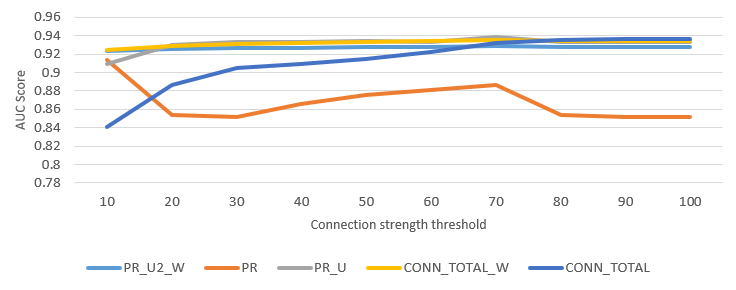
\includegraphics[width=\columnwidth]{ant_SD_LD.PNG}
\caption{Variation of AUC score when varying connection strength threshold for Ant. Results for structural and logical dependencies combined. }
\label{fig:plot_sd_ld_ant}
\centering
\end{figure}


\begin{figure}[H]
\centering
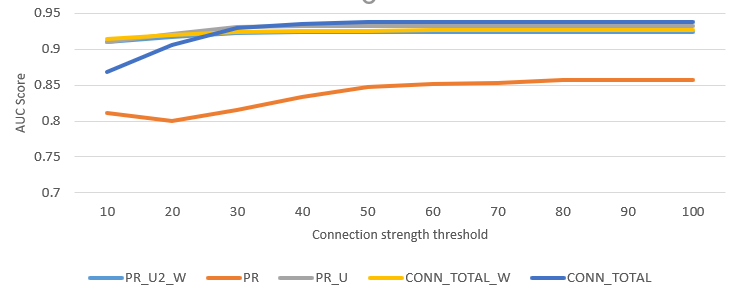
\includegraphics[width=\columnwidth]{tomcat_SD_LD.PNG}
\caption{Variation of AUC score when varying connection strength threshold for Tomcat. Results for structural and logical dependencies combined. }
\label{fig:plot_sd_ld_tomcat}
\centering
\end{figure}


\begin{figure}[H]
\centering
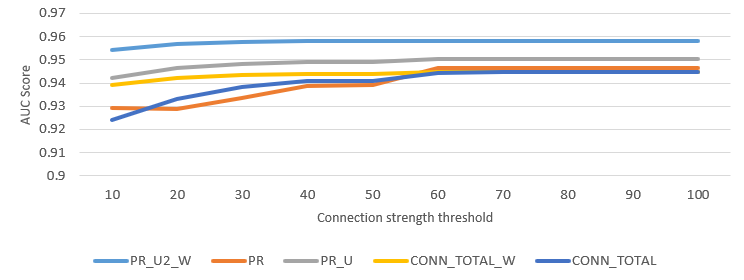
\includegraphics[width=\columnwidth]{hibernate_SD_LD.PNG}
\caption{Variation of AUC score when varying connection strength threshold for Hibernate. Results for structural and logical dependencies combined. }
\label{fig:plot_sd_ld_hibernate}
\centering
\end{figure}



\begin{figure}[H]
\centering
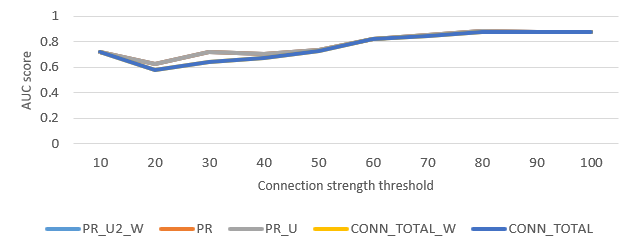
\includegraphics[width=\columnwidth]{ant_LD.PNG}
\caption{Variation of AUC score when varying connection strength threshold for Ant. Results for logical dependencies only. }
\label{fig:plot_ld_ant}
\centering
\end{figure}


\begin{figure}[H]
\centering
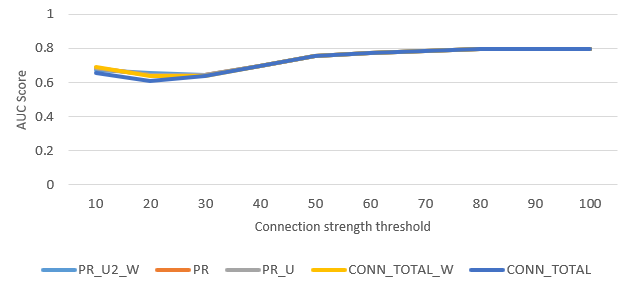
\includegraphics[width=\columnwidth]{tomcat_LD.PNG}
\caption{Variation of AUC score when varying connection strength threshold for Tomcat. Results for logical dependencies only. }
\label{fig:plot_ld_tomcat}
\centering
\end{figure}


\begin{figure}[H]
\centering
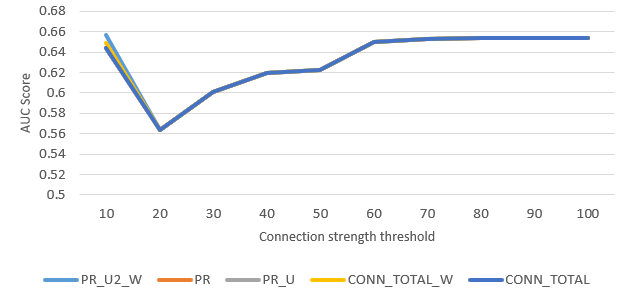
\includegraphics[width=\columnwidth]{hibernate_LD.PNG}
\caption{Variation of AUC score when varying connection strength threshold for Hibernate. Results for logical dependencies only.}
\label{fig:plot_ld_hibernate}
\centering
\end{figure}


The details of the systems are presented in two tables.  In table \ref{tab:overlap} are the overlappings between structural and logical dependencies expressed in percentages. Each column represents the percentage of logical dependencies that are also structural, for each column the logical dependencies are obtained by applying a different connection strength filter. The connection strength filter begins at 10, meaning that in at least 10 \% of the total commits involving two entities, the entities update together. We increase the connection strength filter by 10 up until we reach 100, meaning that in all the commits that involve one entity, the other entity is present also.


In table \ref{tab:ratio_sd_ld} are the ratio numbers between structural dependencies and logical dependencies. We added this table in order to highlight how different the total number of both dependencies is.


\begin{table}[!h]
\renewcommand{\arraystretch}{1}
\caption{Percentage of logical dependencies that are also structural dependencies}
\label{tab:overlap}
\centering
\scalebox{0.7}{
\begin{tabular}{|c|cccccccccc|}
\hline
System &	$\geq10\%$	&	$\geq20\%$		&	$\geq30\%$		&	$\geq40\%$		&	$\geq50\%$		&	$\geq60\%$		&	$\geq70\%$		&	$\geq80\%$		&	$\geq90\%$		&	$\geq100\%$ \\
\hline
Ant	&	25.202	&	34.419	&	36.385	&	34.656	&	33.528	&	33.333	&	28.659	&	33.333	&	35.294	&	35.294	\\
Tomcat Catalina	&	4.059	&	22.089	&	25.000	&	25.758	&	25.926	&	37.525	&	47.368	&	55.285	&	75.000	&	76.923	\\
Hibernate	&	6.546	&	26.607	&	29.565	&	32.374	&	32.543	&	45.170	&	44.980	&	42.473	&	42.473	&	42.473	\\
\hline
\end{tabular}
}
\end{table}



\begin{table}[!h]
\renewcommand{\arraystretch}{1}
\caption{Ratio between structural and logical dependencies (SD/LD)}
\label{tab:ratio_sd_ld}
\centering
\scalebox{0.7}{
\begin{tabular}{|c|cccccccccc|}
\hline
System &	$\geq10\%$	&	$\geq20\%$		&	$\geq30\%$		&	$\geq40\%$		&	$\geq50\%$		&	$\geq60\%$		&	$\geq70\%$		&	$\geq80\%$		&	$\geq90\%$		&	$\geq100\%$ \\
\hline
Ant	&	1.315	&	3.284	&	4.972	&	5.603	&	6.175	&	10.697	&	12.915	&	27.154	&	41.529	&	41.529	\\
Tomcat Catalina	&	0.120	&	0.923	&	1.313	&	1.531	&	1.619	&	3.177	&	7.092	&	13.146	&	67.375	&	124.385	\\
Hibernate	&	1.037	&	6.391	&	10.037	&	14.947	&	18.940	&	54.248	&	83.442	&	111.704	&	111.704	&	111.704	\\

\hline
\end{tabular}
}
\end{table}

In figures \ref{fig:plot_sd_ld_ant}, \ref{fig:plot_sd_ld_tomcat} and \ref{fig:plot_sd_ld_hibernate} are the measurements obtained by using structural and logical dependencies combined. 
In all three figures, the measurements at the beginning are smaller than the rest. Once with the increasing of the threshold value also the measurements begin to increase. Meaning that better results for key class detection are found. 
The best measurements are when the threshold value is between 40 and 60, after that, the measurements tend to decrease a little bit and stay at that fixed value. 

A possible explanation of the results fluctuation and then capping is that if we are looking at table \ref{tab:ratio_sd_ld} we can see that at the beginning, the total number of logical dependencies used is close to the number of existing structural dependencies. The high volume of logical dependencies introduced might cause an erroneous detection of the key classes, in consequence, smaller measurements. 
When the threshold begins to be more restrictive and the total number of logical dependencies used begins to decrease, the key classes detection starts to improve. This improvement stops after the threshold value reaches 60\%. If we look again at table \ref{tab:ratio_sd_ld} we can see that after 60\% the number of structural dependencies outnumbers the number of logical dependencies up to 124 times in some cases. In addition, if we look at table \ref{tab:overlap} we can see that the remaining logical dependencies overlap a lot with the structural dependencies, so we are not introducing too much new information.

 So, the number of logical dependencies used is so small that it doesn't influence the key class identification. Since the structural dependencies used don't change, we obtain the same results for different threshold values. 



In figures \ref{fig:plot_ld_ant}, \ref{fig:plot_ld_tomcat} and \ref{fig:plot_ld_hibernate} are the measurements obtained by using only logical dependencies.
Initially, we expected to see a Gaussian curve, but instead, we see a bell curve.  We think that in the beginning, we use a high number of logical dependencies in key class detection, among those logical dependencies is an important number of key classes and also an important number of other classes. But the number of other classes does not influence the key classes detection. When we start to increase the value of the threshold and filter more the logical dependencies, we also filter some of the initial detected key classes and remain with a significant number of other classes. In this case, the other classes that remain influence the measurements, causing the worst-performing solutions. 
Some of the key classes are strongly connected in the versioning system, and even for higher threshold values don't get filtered out. Meanwhile, the rest of the classes that are not key classes get filtered out for higher threshold values which leads to better performing measurements when the threshold value are above 60\%. 



\section{Comparison of the extracted data with fan-in and fan-out metric}
\label{sec:metrics}

Fan-in and fan-out are coupling metrics. The fan-in of entity A is the total number of entities that call functions of A. The fan-out of A is the total number of entities called by A \cite{5507329}.


In tables \ref{tab:measurementsfan:ant}, \ref{tab:measurementsfan:catalina}, and \ref{tab:measurementsfan:hibernate} we can find the metrics detalis for each documented key class of each system.
The first column represents the name of each key class, the second column represents the fan\_in values for each key class, the third column represents the fan\_out values, the fourth column represents the number of entities that call functions of that key class plus the number of entities that are called by the key class (fan\_in and fan\_out combined), and the fifth column represents the number of logical dependencies in which an entity is involved. 

For Ant, we can see in table \ref{tab:measurementsfan:ant} that all the key classes have logical dependencies with other classes. The LD\_NUMBER means the number of logical dependencies of an entity. The key classes with the most LD number are Project and IntrospectionHelper, these two entities can be found also in table \ref{tab:measurementstop:ant} in which we did a top 10 entities that have a logical dependency with other entities. This means that some key classes are involved in software change quite often and can be observed via system history.

\begin{table}[!h]
\renewcommand{\arraystretch}{1}
\caption{Measurements for Ant key classes}
\label{tab:measurementsfan:ant}
\centering
\scalebox{0.8}{
\begin{tabular}{|c|ccccc|}
\hline
Nr.	&	Classname	&	FAN\_IN	&	FAN\_OUT	&	FAN\_TOTAL	&	LD\_NUMBER\\
\hline
1	&	Project	&	191	&	23	&	214	&	157	\\
2	&	Target	&	28	&	6	&	34	&	78	\\
3	&	UnknownElement	&	17	&	13	&	30	&	90	\\
4	&	RuntimeConfigurable	&	17	&	13	&	30	&	118	\\
5	&	IntrospectionHelper	&	18	&	24	&	42	&	143	\\
6	&	Main	&	1	&	13	&	14	&	82	\\
7	&	TaskContainer	&	11	&	1	&	12	&	21	\\
8	&	ProjectHelper2\$ElementHandler	&	1	&	12	&	13	&	30	\\
9	&	Task	&	110	&	7	&	117	&	88	\\
10	&	ProjectHelper	&	16	&	8	&	24	&	101	\\
\hline
\end{tabular}
}
\end{table}


For Tomcat Catalina, same as for Ant, we can see in table \ref{tab:measurementsfan:catalina} that all the key classes have logical dependencies.  The key classes with the most LD number are StandardContext and Request, these two entities can also be found in table \ref{tab:measurementstop:catalina} in which we did a top 10 entities that have the most logical dependencies with other entities for Tomcat Catalina.

For Hibernate things are a little bit different, as we can see in table \ref{tab:measurementsfan:hibernate},  key classes like Criterion, Projection, or Transaction have 0 logical dependencies, meaning that those key classes are not involved in any software change. One possible explanation for this is that for Hibernate the architecture is designed in such way that the core is not often touched by change. 


\begin{table}[!h]
\renewcommand{\arraystretch}{1}
\caption{Measurements for Tomcat Catalina key classes.}
\label{tab:measurementsfan:catalina}
\centering
\scalebox{0.8}{
\begin{tabular}{|c|ccccc|}
\hline
Nr.	&	Classname	&	FAN\_IN	&	FAN\_OUT	&	FAN\_TOTAL	&	LD\_NUMBER \\
\hline
1	&	Context	&	74	&	8	&	82	&	126	\\
2	&	Request	&	48	&	28	&	76	&	215	\\
3	&	Container	&	51	&	8	&	59	&	64	\\
4	&	Response	&	38	&	12	&	50	&	90	\\
5	&	StandardContext	&	11	&	38	&	49	&	216	\\
6	&	FANector	&	23	&	9	&	32	&	89	\\
7	&	Session	&	29	&	2	&	31	&	28	\\
8	&	Valve	&	29	&	2	&	31	&	19	\\
9	&	Wrapper	&	29	&	1	&	30	&	36	\\
10	&	Manager	&	25	&	3	&	28	&	31	\\
11	&	Host	&	26	&	1	&	27	&	44	\\
12	&	Service	&	20	&	6	&	26	&	51	\\
13	&	Engine	&	23	&	2	&	25	&	1	\\
14	&	Realm	&	18	&	6	&	24	&	21	\\
15	&	CoyoteAdapter	&	1	&	22	&	23	&	140	\\
16	&	StandardHost	&	8	&	15	&	23	&	88	\\
17	&	LifecycleListener	&	21	&	1	&	22	&	3	\\
18	&    StandardEngine	&	2	&	19	&	21	&	57	\\
19	&	Pipeline	&	19	&	2	&	21	&	20	\\
20	&	Server	&	16	&	4	&	20	&	49	\\
21	&	HostConfig	&	3	&	15	&	18	&	79	\\
22	&	StandardWrapper	&	5	&	13	&	18	&	92	\\
23	&	StandardService	&	3	&	12	&	15	&	81	\\
24	&	Catalina	&	2	&	13	&	15	&	94	\\
25	&	Loader	&	14	&	1	&	15	&	18	\\
26	&	StandardServer	&	2	&	12	&	14	&	94	\\
27	&	StandardPipeline	&	1	&	10	&	11	&	62	\\
28	&	Bootstrap	&	3	&	3	&	6	&	41	\\	
\hline
\end{tabular}
}
\end{table}

\begin{table}[!h]
\renewcommand{\arraystretch}{1}
\caption{Measurements for Hibernate key classes.}
\label{tab:measurementsfan:hibernate}
\centering
\scalebox{0.8}{
\begin{tabular}{|c|ccccc|}
\hline
Nr.	&	Classname	&	FAN\_IN	&	FAN\_OUT	&	FAN\_TOTAL	&	LD\_NUMBER \\
\hline
1	&	SessionFactoryImplementor	&	438	&	43	&	481	&	51	\\
2	&	Type	&	444	&	5	&	449	&	0	\\
3	&	Table	&	89	&	29	&	118	&	82	\\
4	&	SessionImplementor	&	52	&	12	&	64	&	14	\\
5	&	Criteria	&	45	&	12	&	57	&	15	\\
6	&	Column	&	46	&	10	&	56	&	20	\\
7	&	Session	&	31	&	21	&	52	&	52	\\
8	&	Query	&	12	&	28	&	40	&	0	\\
9	&	Configuration	&	1	&	38	&	39	&	115	\\
10	&	SessionFactory	&	24	&	12	&	36	&	33	\\
11	&	Criterion	&	30	&	3	&	33	&	0	\\
12	&	Projection	&	11	&	3	&	14	&	0	\\
13	&	FANectionProvider	&	12	&	2	&	14	&	0	\\
14	&	Transaction	&	11	&	1	&	12	&	0	\\
				
\hline
\end{tabular}
}
\end{table}


%%%%%%%%%%%%%%%%%%%%%%%%%%%%%%%%%%%%%%%%%%%%%%%%%%%%%%%%%%%%%%%%%%%%%%%%%%%%%

In tables \ref{tab:measurementstop:ant}, \ref{tab:measurementstop:catalina}, and \ref{tab:measurementstop:hibernate} we can find the top 10 entities with logical dependencies. The first column represents the name of each top 10 entity, the second column represents the fan\_in values, the third column represents the fan\_out values, the fourth column represents the fan\_in and fan\_out combined, and the fifth column represents the number of logical dependencies in which the entity is involved.


We did these top 10 tables to offer an overview of the highest registered numbers for LD for each system. As we mentioned before, some of the key classes are also present in these tables, but not all of them.

In table \ref{tab:measurementstop:hibernate} we can find the top 10 measurements for Hibernate, most of the table is occupied by inner classes of AbstractEntityPersister. This is expected behavior since class AbstractEntityPersister is also present. This behavior is caused by the impossibility to separate the updates done for a class from its inner classes in the versioning system. So, each time AbstractEntityPersister records a change, also the inner classes are considered to have changed.
\begin{table}[!h]
\renewcommand{\arraystretch}{1}
\caption{Top 10 measurements for Ant. }
\label{tab:measurementstop:ant}
\centering
\scalebox{0.8}{
\begin{tabular}{|c|ccccc|}
\hline
Nr.	&	Classname	&	FAN\_IN	&	FAN\_OUT	&	FAN\_TOTAL	&	LD\_NUMBER \\
\hline
1	&	\cellcolor{lightorange}Project	&	191	&	23	&	214	&	157	\\
2	&	Project\$AntRefTable	&	1	&	2	&	3	&	157	\\
3	&	Path	&	39	&	13	&	52	&	147	\\
4	&	Path\$PathElement	&	3	&	2	&	5	&	147	\\
5	&	\cellcolor{lightorange}IntrospectionHelper	&	18	&	24	&	42	&	143	\\
6	&	IntrospectionHelper\$AttributeSetter	&	8	&	1	&	9	&	143	\\
7	&	IntrospectionHelper\$Creator	&	3	&	5	&	8	&	143	\\
8	&	IntrospectionHelper\$NestedCreator	&	7	&	1	&	8	&	143	\\
9	&	Ant	&	2	&	15	&	17	&	136	\\
10	&	Ant\$Reference	&	3	&	1	&	4	&	136	\\
\hline
\end{tabular}
}
\end{table}

\begin{table}[!h]
\renewcommand{\arraystretch}{1}
\caption{Top 10 measurements for Tomcat Catalina. }
\label{tab:measurementstop:catalina}
\centering
\scalebox{0.8}{
\begin{tabular}{|c|ccccc|}
\hline
Nr.	&	Classname	&	FAN\_IN	&	FAN\_OUT	&	FAN\_TOTAL	&	LD\_NUMBER \\
\hline
1	&	\cellcolor{lightorange}StandardContext	&	11	&	38	&	49	&	216	\\
2	&	StandardContext\$ContextFilterMaps	&	0	&	0	&	0	&	216	\\
3	&	StandardContext\$NoPluggabilityServletContext	&	0	&	0	&	0	&	216	\\
4	&	\cellcolor{lightorange}Request	&	48	&	28	&	76	&	215	\\
5	&	Request\$SpecialAttributeAdapter	&	0	&	0	&	0	&	215	\\
6	&	ApplicationContext	&	3	&	22	&	25	&	158	\\
7	&	ApplicationContext\$DispatchData	&	0	&	0	&	0	&	158	\\
8	&	ContextConfig	&	3	&	26	&	29	&	143	\\
9	&	ContextConfig\$DefaultWebXmlCacheEntry	&	0	&	0	&	0	&	143	\\
10	&	ContextConfig\$JavaClassCacheEntry	&	0	&	0	&	0	&	143	\\
\hline
\end{tabular}
}
\end{table}


\begin{table}[!h]
\renewcommand{\arraystretch}{1}
\caption{Top 10 measurements for Hibernate. }
\label{tab:measurementstop:hibernate}
\centering
\scalebox{0.8}{
\begin{tabular}{|c|ccccc|}
\hline
Nr.	&	Classname	&	FAN\_IN	&	FAN\_OUT	&	FAN\_TOTAL	&	LD\_NR \\
\hline
1	&	AvailableSettings	&	1	&	0	&	1	&	205	\\
2	&	AbstractEntityPersister	&	9	&	143	&	152	&	190	\\
3	&	AbstractEntityPersister\$CacheEntryHelper	&	0	&	0	&	0	&	190	\\
4	&	AbstractEntityPersister\$InclusionChecker	&	0	&	0	&	0	&	190	\\
5	&	AbstractEntityPersister\$NoopCacheEntryHelper	&	0	&	0	&	0	&	190	\\
6	&	AbstractEntityPersister\$ReferenceCacheEntryHelper	&	0	&	0	&	0	&	190	\\
7	&	AbstractEntityPersister\$StandardCacheEntryHelper	&	0	&	0	&	0	&	190	\\
8	&	AbstractEntityPersister\$StructuredCacheEntryHelper	&	0	&	0	&	0	&	190	\\
9	&	Dialect	&	265	&	104	&	369	&	176	\\
10	&	SessionFactoryImpl\$SessionBuilderImpl	&	1	&	25	&	26	&	167	\\
\hline
\end{tabular}
}
\end{table}

Overall, by looking at the comparisons between FAN\_IN, FAN\_OUT, FAN\_TOTAL, and the logical dependencies in which a class is involved we could not determine a direct connection between them. Nither we can say that one influences the other.  We consider that even though the metrics are not related directly, they could be all used together to get a better view of the system connections.


\chapter{Logical dependencies in architectural reconstruction}

We explore using code co-changes as input for software clustering for architectural reconstruction. Since structural dependencies are the most commonly used dependencies in software clustering, we investigate whether integrating them with code co-changes provides better results than using either dependency type alone.

Our experiments are applied to four open-source Java projects from GitHub. For each project, we apply three distinct clustering algorithms (Louvain, Leiden, and DBSCAN) and evaluate their performance using two clustering evaluation metrics. These metrics allow a comparison between clustering based solely on code co-changes and clustering that integrates both co-changes and structural dependencies, offering a better understanding of how these co-changes influence software architecture reconstruction.


\section{Introduction}
\label{sec:introduction_clustering}

Software systems often need more documentation. Even if there was original documentation at the beginning of development, it may become outdated over the years. Additionally, the original developers may leave the company, taking with them knowledge about how the software was designed. This situation challenges the teams when it comes to maintenance or modernization. In this context, recovering the system's architecture is essential. Understanding the system's architecture helps developers evaluate better and understand the nature and impact of changes they must make. One technique to help in reconstructing the system architecture is software clustering. Software clustering involves creating cohesive groups (modules) of software entities based on their dependencies and interactions.

Among the dependencies that can be used for software clustering are structural dependencies (relationships between entities based on code analysis), lexical dependencies (relationships based on naming conventions), and code co-changes/logical dependencies (relationships between entities extracted from the version control system), and others.

This paper assesses the impact of logical dependencies in software clustering alone and combination with structural dependencies. The structural dependencies are used as they are extracted from static code analysis, while the logical dependencies are filtered co-changes obtained from the version control system \cite{b15}. The co-changes are filtered to enhance their reliability and remove noise caused by large commits with many files unrelated to development activities (e.g., formatting changes) or rare co-changes that may not indicate a true dependency \cite{b1}.

The following research questions guide our investigation:

\begin{itemize}
\item \textbf{RQ1:} Does using structural dependencies (SD) combined with logical dependencies (LD) improve software clustering results compared to traditional approaches using only structural dependencies (SD)?
\item \textbf{RQ2:} Can using only logical dependencies (LD) produce good software clustering results?
\item \textbf{RQ3:} How do different filtering settings for logical dependencies (LD) impact clustering results, and which filtering settings provide the best performance?
\end{itemize}

To answer these research questions, we apply three different clustering algorithms (Louvain, Leiden, and DBSCAN) to different open-source projects. We then evaluate the results using two metrics: MQ (Modularization Quality) \cite{b10} and MoJoFM (Move and Join e\textbf{F}fectiveness \textbf{M}easure) \cite{mojofm}. The MoJoFM metric is used for external evaluation, evaluating against the perspective of the system's architect or developers. The MQ metric is used for internal evaluation based on the software structure itself. These two metrics allow us to compare the effectiveness of using structural and logical dependencies alone and combined. This comparison helps clarify how different dependencies and filtering choices affect clustering results.



\section{Related work}
\label{sec:related_work}

Several studies have explored the use of different types of dependencies in software clustering, applying different algorithms to improve clustering results and using various metrics to evaluate the results obtained.

Tzerpos and Holt developed ACDC (Algorithm for Comprehension-Driven Clustering). This pattern-driven clustering algorithm uses subsystem structures such as source file patterns, directory patterns, system graph patterns, and support library patterns to detect similarities and create clusters \cite{acdc}. For result evaluation, the authors introduced the MoJo metric, which counts the minimum number of move and join operations required to transform one clustering result into another, assessing how close one clustering solution is to another \cite{b3}, \cite{tzerpos1}. Later, Wen and Tzerpos introduced the MoJoFM metric, an enhanced version of the original MoJo distance metric for more effective measurements, as presented in more detail in subsection \ref{subsec:mojofm} \cite{mojofm}.

Corazza et al. \cite{lexical-dep}, \cite{corazza2} used lexical dependencies derived from code comments, class names, attribute names, and parameter names, applying Hierarchical Agglomerative Clustering (HAC) to group-related entities. For evaluating the results, the authors used a metric based on the MoJo distance metric and NED (Non-Extremity Cluster Distribution), which measures that the formed clusters are not too large or too small.

Andritsos and Tzerpos ~\cite{tzerpos1} used structural dependencies and nonstructural attributes, such as file names and developer names, and proposed the LIMBO algorithm, a hierarchical clustering algorithm for clustering software systems. They used the MoJo distance metric to evaluate the algorithm's output.

Anquetil et al.~\cite{b14} also used lexical information, including file names, routine names, included files, and comments. They applied an n-gram-based clustering approach to detect semantic similarities between entities and evaluated the results using precision and recall metrics.

Maletic and Marcus \cite{maletic} propose an approach to software clustering that uses semantic dependencies extracted using Latent Semantic Indexing (LSI), a technique for identifying similarities between software components. They apply the minimal spanning tree (MST) algorithm for clustering and evaluate the results using metrics based on both semantic and structural information.

Wu et al. \cite{wu} conducted a comparative study of six clustering algorithms using structural dependencies on five software systems. Four of the algorithms are based on agglomerative clustering, one on program comprehension patterns, and one algorithm is a customized version of Bunch \cite{b10}. The performance of these algorithms was evaluated using the MoJo metric and NED (Non-Extreme Distribution).

Mancoridis and Mitchell ~\cite{b10}, \cite{b2}, \cite{bunch} developed the Bunch tool for software clustering and used structural dependencies as input. The tool applies clustering algorithms to the structural dependency graph and outputs the system's organization. For evaluation, the authors introduced the Modularization Quality (MQ) metric, described in more detail in Section \ref{subsec:mq}, and is also used in our current experiments as an evaluation metric.


Prajapati et al.~\cite{b18} propose a many-objective SBSR (search-based software remodularization) approach with an improved definition of objective functions based on lexical, structural, and change-history dependencies. The authors evaluate their approach on several open-source software systems using the MoJoFM metric for external evaluation and the MQ metric for internal evaluation.

Şora et al.~\cite{SoraSem13}, \cite{SoraConti} developed the ARTs (Architecture Reconstruction Tool Suite) for their experiments on improving software architecture reconstruction through clustering. The tool suite implements various clustering algorithms, such as minimum spanning tree-based, metric-based, search-based, and hierarchical clustering, primarily using structural dependencies as input. The research focuses on identifying the right factors for direct coupling between classes, indirect coupling, and layered architecture. The results of applying these different factors are evaluated using the MoJo distance metric.

Silva et al.~\cite{b16} investigated using solely co-change dependencies as input for the Chameleon algorithm, an agglomerative hierarchical clustering method, to identify clusters. For evaluation, the authors used distribution maps to compare the clusters generated from co-change dependencies with the system's package structure.


%%%%%%%%%%%%%%%%%%%%%%%%%%%%%%%%%%%%%%%%%%%%%%%%%%%%%


\section{Methodology and implementation}
\label{sec:methodology_implementation}

In this section, we present the methodology used to evaluate the impact of logical dependencies on the quality of software clustering solutions.

First, we describe the clustering algorithms used in our experiments: Louvain, Leiden, and DBSCAN. Next, we introduce the evaluation metrics used to assess the quality of the clustering results. Finally, we present the workflow and implementation of the tool developed for this research, which is built to process structural and logical dependencies, apply the selected clustering algorithms, and compute the evaluation metrics.

\subsection{Clustering algorithms}
\subsubsection{Louvain}
\label{subsubsec:louvain}

The Louvain algorithm was originally developed by Blondel et al. and is used to find community partitions (clusters) in large networks. The algorithm begins with a weighted network of N nodes, initially assigning each node to its own cluster, resulting in N clusters. For each node, the algorithm evaluates the modularity gained from moving the node to the cluster of each of its neighbors. Based on the results, the node is moved to the cluster with the maximum positive modularity gain. This process is repeated for all nodes until no further improvement in modularity is possible \cite{b8}, \cite{b9}.

\subsubsection{Leiden}
\label{subsubsec:leiden}

The Leiden algorithm, developed by Traag et al., is an improvement over the Louvain algorithm for community detection in large networks. Like Louvain, the Leiden algorithm begins with each node assigned to its own cluster and iteratively moves nodes between clusters to optimize modularity. However, the Leiden algorithm addresses some problems of the Louvain method, particularly regarding poorly connected communities and runtime performance issues \cite{leiden} \cite{scikit}.

The Leiden algorithm introduces a refinement phase that ensures communities are locally optimally clustered and well-connected. This refinement step distinguishes the Leiden algorithm from Louvain.


\subsubsection{DBSCAN}
\label{subsubsec:dbscan}

The Density-Based Spatial Clustering of Applications with Noise (DBSCAN) algorithm, introduced by Ester et al., is a density-based clustering algorithm for identifying clusters of arbitrary shape and detecting noise in data \cite{dbscan}, \cite{scikit}.

DBSCAN operates based on two main parameters:

\begin{itemize}
\item \textbf{Eps}: It defines the radius within which to search for neighboring points.
\item \textbf{MinPts}: The minimum number of points required for a dense region. It determines the minimum number of neighbors a point should have to be considered a core point.
\end{itemize}

The algorithm classifies points into three categories:

\begin{enumerate}
\item \textbf{Core Points}: Points that have at least \textit{MinPts} neighbors within a radius of \textit{Eps}. These points are located in the interior of a cluster.
\item \textbf{Border Points}: Points that have fewer than \textit{MinPts} neighbors within a radius of \textit{Eps} but are in the Eps-neighborhood of a core point. They are located on the edge of a cluster.
\item \textbf{Noise}: Points that are neither core points nor border points.
\end{enumerate}

The DBSCAN algorithm starts by visiting an arbitrary point in the dataset. If the point is a core point, the algorithm starts a new cluster and retrieves all reachable points from this core point. All points are then marked as part of the cluster. If the point is a border point, it moves to the next point in the dataset. This process is repeated until all points have been visited.

DBSCAN can be applied for software clustering by considering software entities as data points. A distance measure based on dependency weights can be used to compute the neighborhood between entities.

\subsection{Clustering result evaluation}
\label{subsec:evaluation_def}

We evaluate the clustering results using two metrics: the Modularity Quality (MQ) metric and the Move and Join Effectiveness Measure (MoJoFM) metric. Each provides a different perspective on the quality of the clustering solutions.

\subsubsection{Modularity Quality metric}
\label{subsec:mq}

Mancoridis et al. introduced the Modularity Quality (MQ) metric to evaluate the modularization quality of a clustering solution based on the interaction between modules (clusters) \cite{b101},\cite{b10}. It evaluates the difference between connections within clusters and connections between different clusters.

The MQ of a graph partitioned into \( k \) clusters, where \( A_i \) is the Intra-Connectivity of the \( i \)-th cluster and \( E_{ij} \) is the Inter-Connectivity between the \( i \)-th and \( j \)-th clusters, is calculated using Equation \eqref{eq:mq} \cite{b2}.

\begin{equation}
MQ = \left( \frac{1}{k} \sum_{i=1}^{k} A_i \right) - \left( \frac{1}{k(k-1)} \sum_{i,j=1}^{k} E_{ij} \right)
\label{eq:mq}
\end{equation}

The MQ metric's value ranges between -1 and 1. A value of -1 means that the clusters have more connections between the clusters than within the clusters, while a value of 1 means that there are more connections within clusters than between clusters. A good clustering solution should have an MQ value close to 1, since this indicates that the clusters are more cohesive internally and have fewer connections to other clusters.

The MQ metric is useful because it does not require additional input besides the clustering result. It relies on the structure of the clustered entities and their interactions.

\subsubsection{MoJoFM metric}
\label{subsec:mojofm}
Wen and Tzerpos introduced the MoJoFM metric to evaluate the similarity between two different software clustering results \cite{mojofm}. The metric is based on the MoJo metric, which measures the absolute minimum number of \textit{Move} and \textit{Join} operations required to transform one clustering solution into another \cite{b3}, \cite{mojofm}. However, MoJoFM provides a similarity measure ranging between 0\% and 100\%, where 100\% indicates identical clustering solutions.

The MoJoFM metric is calculated using Equation \eqref{eq:mojofm}:

\begin{equation}
\text{MoJoFM}(A, B) = \left(1 - \frac{\text{mno}(A, B)}{\max(\text{mno}(\forall A, B))}\right) \times 100\%
\label{eq:mojofm}
\end{equation}

Where:

\begin{itemize}
\item $\text{mno}(A, B)$ is the minimum number of \textit{Move} and \textit{Join} operations required to transform clustering solution $A$ into clustering solution $B$.
\item $\max(\text{mno}(\forall A, B))$ is the maximum possible number of such operations required to transform any clustering $A$ into clustering $B$.
\end{itemize}

To use the metric, we first need to generate a reference clustering solution for comparison. We manually created this reference based on our analysis of the codebase.

Using the MoJoFM metric, we can evaluate the similarity between the generated and reference clustering solutions. This metric is useful when combining multiple dependencies because it measures the similarity between the obtained clustering solutions and the same reference.


\subsection{Tool workflow for software clustering and evaluation}
\label{subsec:tool_workflow}


\begin{figure}[t!]
  \centering
  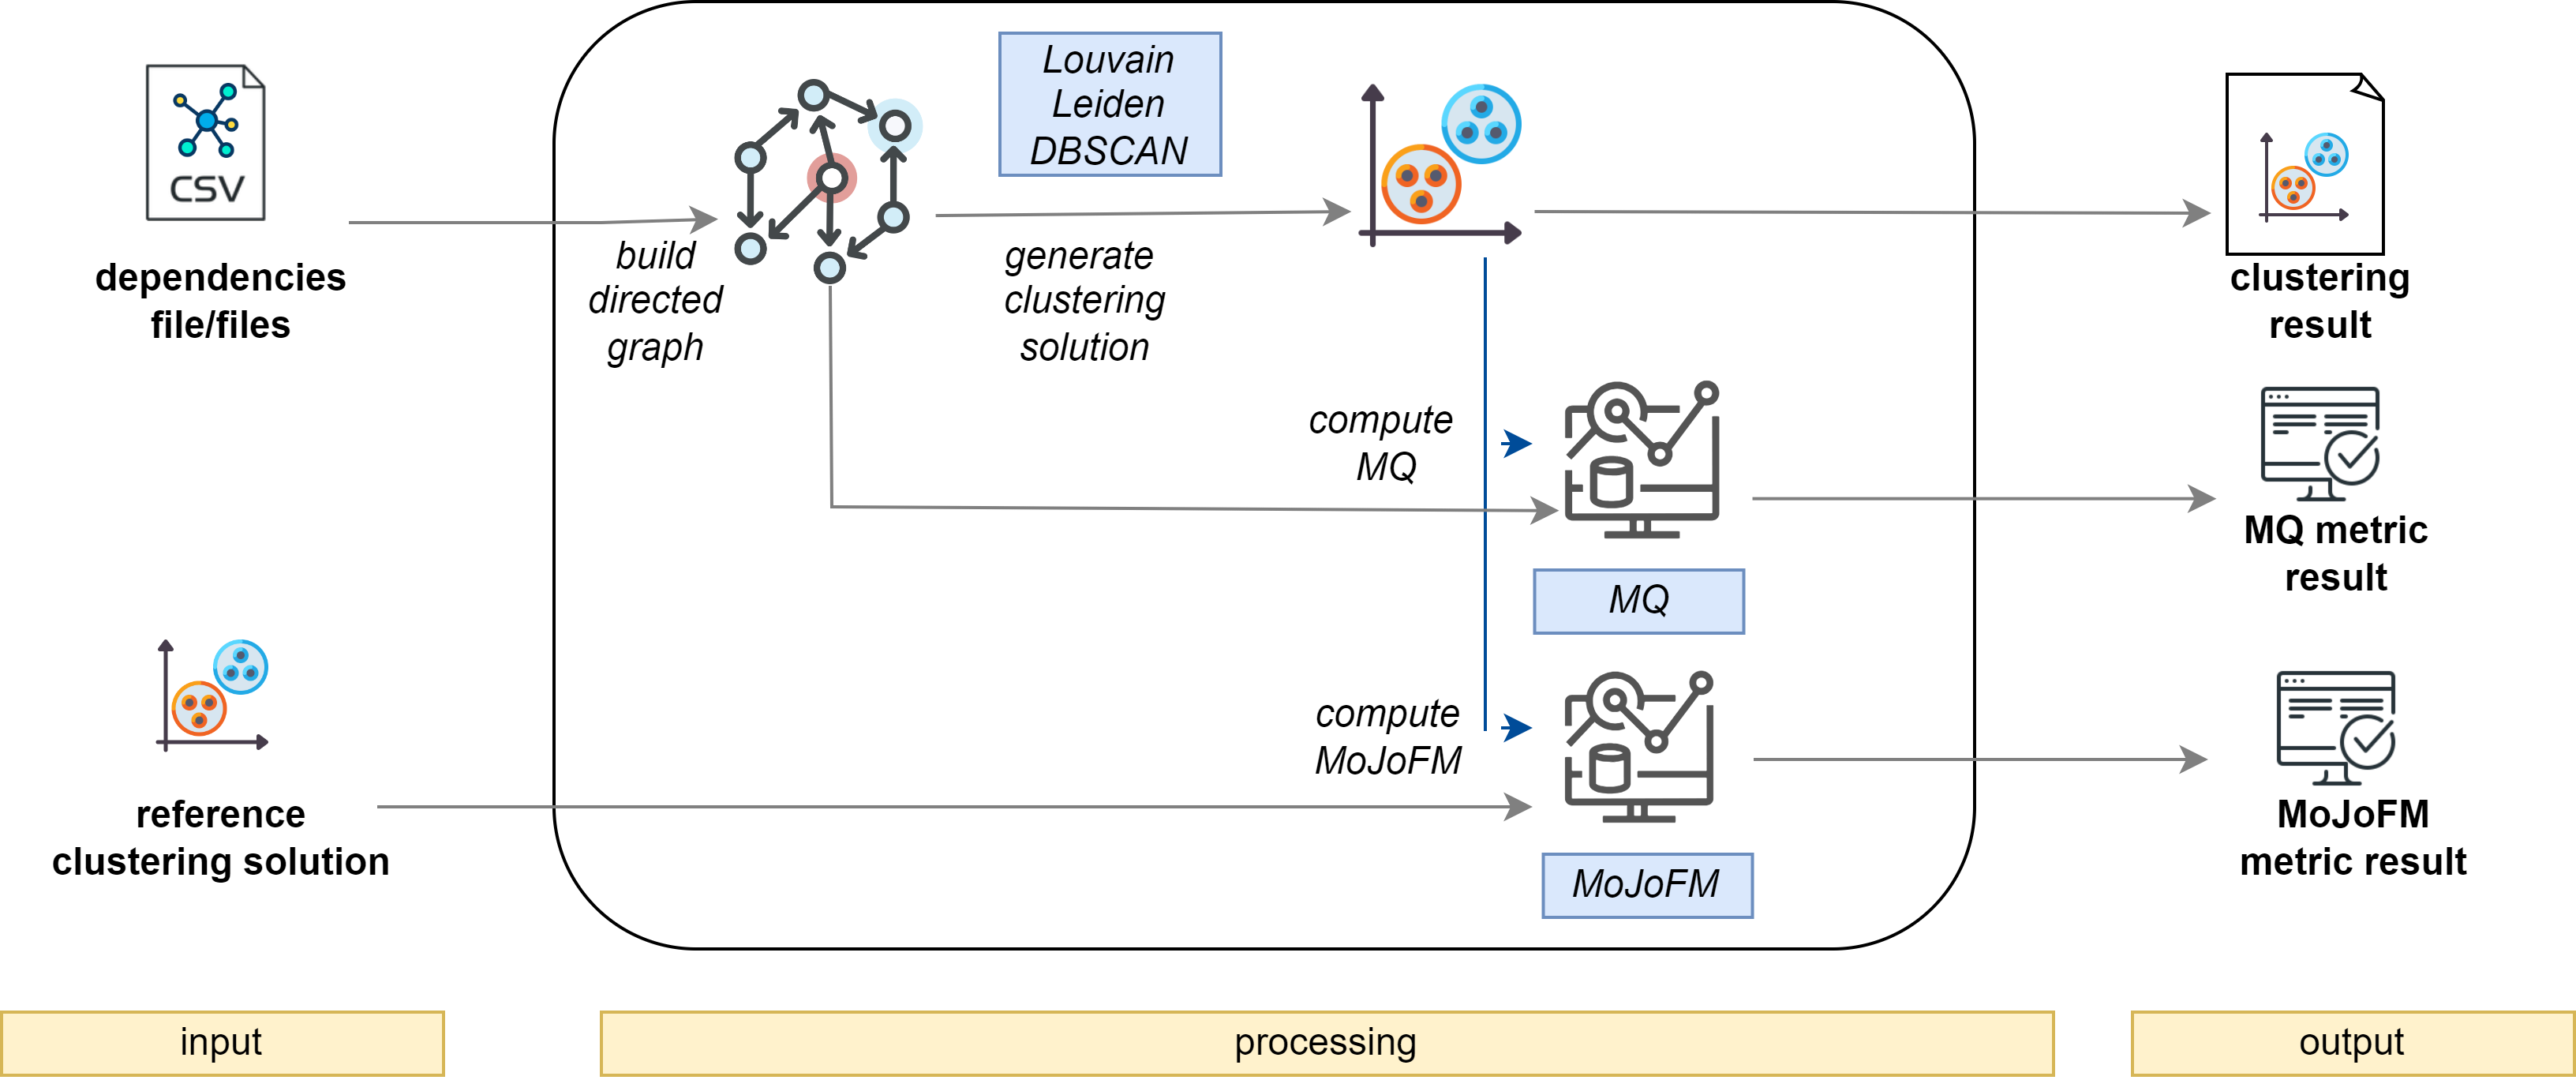
\includegraphics[width=\columnwidth]{workflow-tool.png}
  \caption{ Tool workflow overview: input, processing and output.}
  \label{fig:tool}
\end{figure}

To evaluate how logical dependencies impact the quality of clustering solutions, we developed a Python tool capable of using any type of dependency, either alone or combined with other types of dependencies, as long as it is provided in CSV format. The tool clusters and evaluates software clustering solutions using the MQ or MoJoFM metrics.



\subsubsection{Input}

The tool takes one or multiple dependency CSV files as input and the reference solution required for the MoJoFM metric. We designed the tool to accept multiple dependency files so that we can generate clustering solutions based on either a single type of dependency (structural or logical) or a combination of both.

Since the MoJoFM metric requires a reference solution to evaluate the obtained clustering solutions, we manually inspected the code and created reference clustering solutions, which we then provided as input for the tool.

\subsubsection{Processing}

The dependencies are saved in the CSV file in the following format: \texttt{antecedent of a dependency, consequent of a dependency, weight}. The tool reads each line, adds the antecedent and consequent as nodes in a directed graph, and creates an edge between them, with the weight from the CSV file becoming the edge weight. The edge weights are summed if multiple dependency files are processed and the same dependency is found in multiple files.

The workflow of applying the clustering algorithms and performing the evaluations is shown in Figure \ref{fig:tool}. After all dependencies are read, the directed graph is passed to the clustering algorithms: Louvain, Leiden, and DBSCAN. Each algorithm generates its own clustering result. The results from each algorithm are then evaluated using the MQ metric and the MoJoFM metric. The MQ metric requires the directed graph and the clustering result, while the MoJoFM metric requires the reference clustering solution provided as input and the clustering result.


\subsubsection{Output}

After applying each clustering algorithm and completing both evaluations, we export the clustering result, the number of clusters from the clustering solution, and the MQ and MoJoFM metrics values.


%%%%%%%%%%%%%%%%%%%%%%%%%%%%%%%%%%%%%%%%%%%%%%%%%%%%%%%%%%

\section{Data set used in experimental analysis}

\begin{table}[!h]
\renewcommand{\arraystretch}{1}
\centering
\caption{Overview of projects used in experimental analysis}
\label{tab:project_info}
\scalebox{0.7}{
\begin{tabular}{|c|c|c|c|p{3cm}|}
\hline
\textbf{Project Name} & \textbf{Release Tag} & \textbf{Commits} & \textbf{GitHub Repository Link} & \textbf{Repository Description} \\ \hline
Apache Ant & 1.10.13 & 14,917 & https://github.com/apache/ant & Java build tool for automating software tasks. \\ \hline
Apache Tomcat & 8.5.93 & 22,698 & https://github.com/apache/tomcat & Java web server and servlet container. \\ \hline
Hibernate ORM & 6.2.14 & 16,609 & https://github.com/hibernate/hibernate-orm & Java ORM framework for database management. \\ \hline
Gson & gson-parent-2.10.1 & 1,772 & https://github.com/google/gson & Java library for JSON serialization and deserialization. \\ \hline
\end{tabular}
}
\end{table}

In Table \ref{tab:project_info}, we have synthesized all the information about the four projects used in our experiments. The 'Project Name' column contains the names of the software projects sourced from GitHub. The 'Release Tag' column contains the specific release tag of the project that was analyzed. We processed all the commits for logical dependency extraction, from the first commit to the commit associated with the specified tag. We extracted the dependencies from the code of that specific tag for structural dependencies. The 'Number of Commits' column provides the total number of commits used for logical dependencies extraction. The 'GitHub Repository Link' column includes the URL link to the project's repository on GitHub. Finally, the 'Repository Description' column briefly describes the project's purpose and functionality.

We mainly chose projects with more than 10,000 commits in their commit history so that the logical dependencies extraction can be done on a more extensive information base. However, we selected Gson, which has a relatively small commit history (1,772 commits), to determine if our experiments work with a smaller information base.

Table \ref{tab:commit_statistics} presents the commit statistics for the studied projects. The columns represent the percentage of commits with under 5 files modified, between 5 and 10 files, between 10 and 20 files, and above 20 files modified. We can observe that most commits have under 5 files changed, with Apache Tomcat having more than 90\% of the commits with less than 5 files changed. On the opposite side, only a few commits involve more than 20 files changed, Hibernate ORM having the highest percentage at 8.39\%. 

\begin{table}[ht]
    \centering
    \caption{Commit statistics for studied projects}
    \label{tab:commit_statistics}
\scalebox{0.7}{
    \begin{tabular}{|l|c|c|c|c|c|}
        \hline
	 \textbf{Project Name} & \multicolumn{4}{c|}{\textbf{{Number of files changed} }}  \\ 
	\cline{2-5}
         & \textbf{Under 5} & \textbf{5-10} & \textbf{10-20} & \textbf{Above 20} \\ \hline
        Apache Ant & 83.83\% & 7.50\% & 4.17\% & 4.50\% \\ 
        Apache Tomcat & 90.95\% & 5.44\% & 2.04\% & 1.58\%  \\ 
        Hibernate ORM & 71.74\% & 12.37\% & 7.50\% & 8.39\%  \\ 
        Gson & 83.63\% & 9.85\% & 3.70\% & 2.81\%  \\ \hline
    \end{tabular}
}
\end{table}

\section{Experimental plan and results}
\label{sec:experiment}


\subsection{Experimental plan}
\label{subsec:plan}

\subsubsection{Tool runs}

To assess the impact of logical dependencies and to answer the research questions from section \ref{sec:introduction_clustering}, we run the tool presented in Section \ref{subsec:tool_workflow} in three different scenarios for all the projects from table \ref{tab:project_info}. All three scenarios are illustrated in Fig. \ref{fig:scenatrio}.

In the first scenario, we run the tool once, providing only the system's structural dependencies as input for the clustering algorithm.

In the second scenario, we run the tool ten times, using only logical dependencies as input. We perform ten runs because we generate logical dependencies with different threshold values for the strength filter. We start with a threshold of 10 and increase it in steps of 10 up to 100, where 100 is the maximum value for the threshold.

In the third scenario, we combine logical with structural dependencies. Similar to the second scenario, we ran the tool ten times using structural and logical dependencies generated with different strength thresholds.

\begin{figure}[t!]
  \centering
  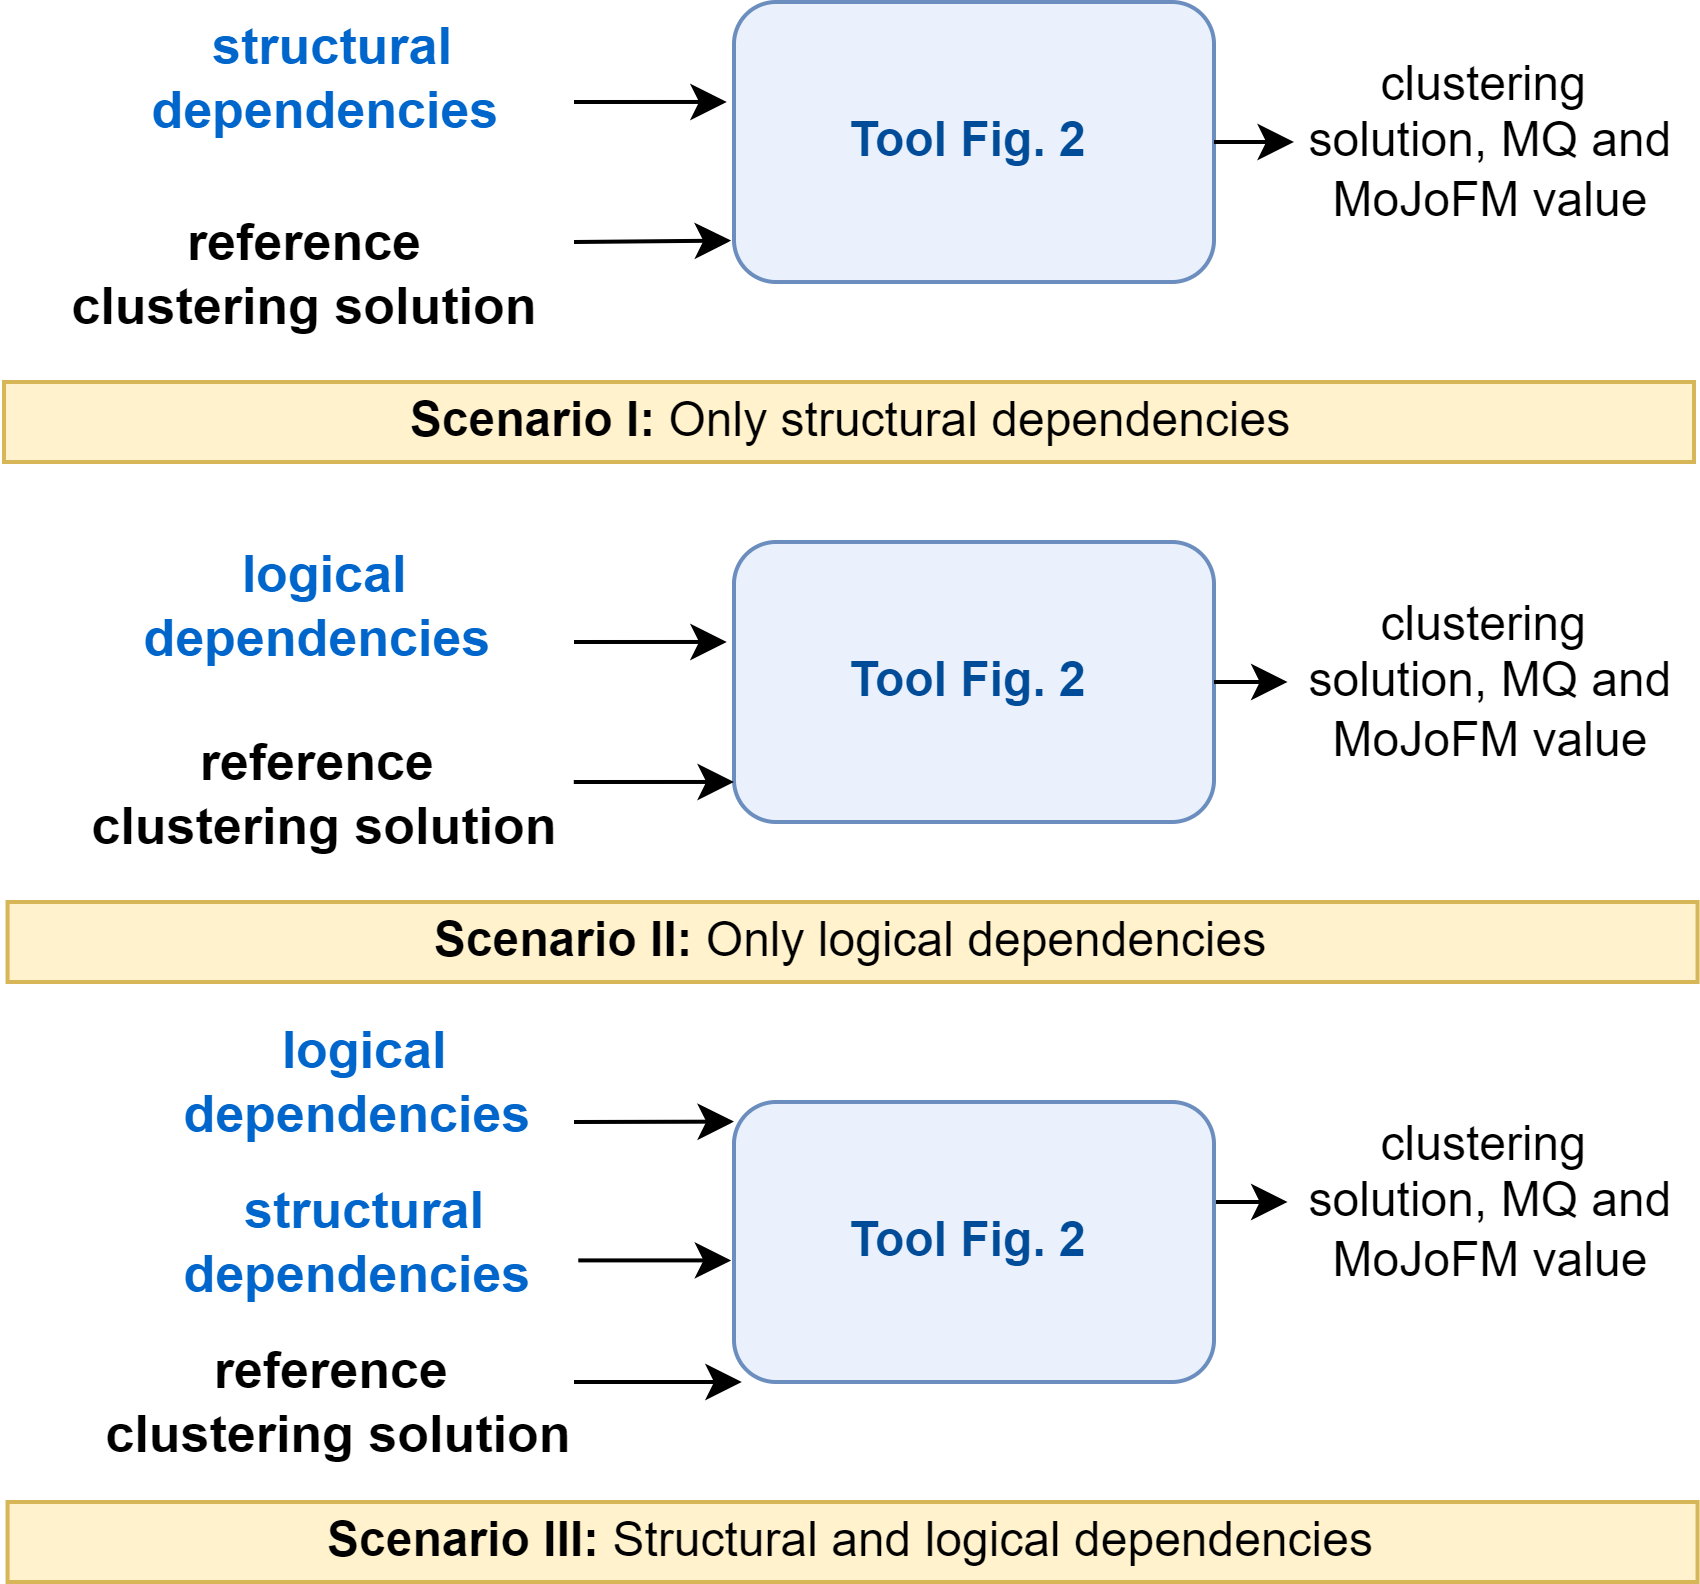
\includegraphics[width=\columnwidth]{scenario.png}
  \caption{ Experimental scenarios for analyzing the impact of logical dependencies on clustering quality}
  \label{fig:scenatrio}
\end{figure}

\subsection{Results}
\label{subsec:results}

The experimental results are presented in this subsection in four tables, each corresponding to a different project. Table \ref{tab:clustering_results_ant} presents the results for Apache Ant, Table \ref{tab:clustering_results_tomcat} presents the results for Apache Tomcat, Table \ref{tab:clustering_results_hibernate} presents the results for Hibernate ORM, and Table \ref{tab:clustering_results_gson} presents the results for Gson.

Each table includes the following columns:
\begin{itemize}
\item \textbf{Dependency Type:} The types of dependencies used are as follows: SD for Structural Dependencies, LD for Logical Dependencies, and SD+LD for their combination. The strength threshold used is specified in parentheses right after LD.
\item \textbf{Entities Count:} The total number of software entities (such as classes, interfaces, enums) involved in clustering.
\item \textbf{System Coverage:} Considering that the total number of entities extracted from the codebase — which represents the entities forming structural dependencies (SD) — constitutes the entire set of entities in the system (the first line of each table), we calculated the percentage of entities present in the filtered logical dependencies (LD) relative to the total number of known codebase entities.
\item \textbf{Louvain/ Leiden/ DBSCAN:} The clustering algorithms used in the experiments.
\item \textbf{Nr. of Clusters:} The number of clusters from the clustering solution.
\item \textbf{MQ (Modularization Quality):} The result obtained when applying the MQ evaluation metric to the clustering solution.
\item \textbf{MoJoFM:} The result obtained when applying the MoJoFM evaluation metric to the clustering solution.
\end{itemize}

The rows in each table represent different dependency types and strength filter thresholds used in the clustering experiments.



\begin{table}[htbp]
\centering
\caption{Clustering results based on different dependency types and strength filter thresholds for repository: https://github.com/apache/ant}
\label{tab:clustering_results_ant}
\resizebox{\textwidth}{!}{
\begin{tabular}{|l|c|c|ccc|ccc|ccc|}
\hline
 \textbf{Dependency} &  \textbf{Entities} & \textbf{System} & \multicolumn{3}{c|}{\textbf{Louvain}} & \multicolumn{3}{c|}{\textbf{Leiden}} & \multicolumn{3}{c|}{\textbf{DBSCAN}} \\
\cline{4-12}
\textbf{Type (strength } &  \textbf{Count} & \textbf{Coverage} & \textbf{Nr. of } & \textbf{MQ} & \textbf{MojoFM} & \textbf{Nr. of} & \textbf{MQ} & \textbf{MojoFM} & \textbf{Nr. of} & \textbf{MQ} & \textbf{MojoFM}  \\
\textbf{threshold)} &  & \textbf{(\%)} & \textbf{clusters} & & & \textbf{clusters} & &  & \textbf{clusters} & &\\
\hline
\rowcolor[HTML]{ECECEC} \textbf{SD} & 517 & 100.00 & 14 & 0.114 & 46.02 & 14 & 0.101 & 52.99 & 34 & 0.144 & 25.1  \\
\textbf{LD (10)} & 320 & 61.89 & 55 & 0.506 & 65.57 & 55 & 0.506 & 65.57 & 30 & 0.435 & 39.02 \\
\textbf{LD (20)} & 215 & 41.58 & 53 & 0.547 & 68 & 53 & 0.547 & 68 & 23 & 0.505 & 53.5 \\
\textbf{LD (30)} & 174 & 33.65 & 44 & 0.558 & 71.7 & 44 & 0.558 & 71.7 & 19 & 0.585 & 50 \\
\textbf{LD (40)} & 152 & 29.40 & 40 & 0.580 & 71.53 & 40 & 0.580 & 71.53 & 19 & 0.602 & 53.06 \\
\textbf{LD (50)} & 138 & 26.69 & 35 & 0.604 & 73.98 & 35 & 0.604 & 73.98 & 17 & 0.633 & 56.1 \\
\textbf{LD (60)} & 120 & 23.21 & 34 & 0.587 & 70.48 & 34 & 0.587 & 70.48 & 14 & 0.650 & 51.43 \\
\textbf{LD (70)} & 106 & 20.50 & 32 & 0.577 & 71.43 & 32 & 0.577 & 71.43 & 11 & 0.661 & 51.65 \\
\textbf{LD (80)} & 92 & 17.79 & 29 & 0.576 & 70.13 & 29 & 0.576 & 70.13 & 9 & \cellcolor[HTML]{FEF9E4}0.709 & 50.65 \\
\textbf{LD (90)} & 79 & 15.28 & 24 & 0.606 & 71.88 & 24 & 0.606 & 71.88 & 8 & 0.705 & 56.6 \\
\textbf{LD (100)} & 64 & 12.37 & 19 & \cellcolor[HTML]{fef9e4}0.611 & \cellcolor[HTML]{fef9e4}75.51 & 19 & \cellcolor[HTML]{fef9e4}0.611 & \cellcolor[HTML]{fef9e4}75.51 & 6 & 0.691 & \cellcolor[HTML]{fef9e4}56.93 \\
\hline
\textbf{SD+LD (10)} & 517 & 100.00 & 18 & \cellcolor[HTML]{fef9e4}0.355 & \cellcolor[HTML]{fef9e4}55.18 & 15 & 0.254 & \cellcolor[HTML]{fef9e4}54.98 & 37 & 0.147 & 25.9 \\
\textbf{SD+LD (20)} & 517 & 100.00 & 17 & 0.318 & 52.39 & 19 & \cellcolor[HTML]{fef9e4}0.365 & 53.78 & 32 & 0.149 & \cellcolor[HTML]{fef9e4}26.49 \\
\textbf{SD+LD (30)} & 517 & 100.00 & 16 & 0.282 & 53.19 & 16 & 0.265 & 54.78 & 30 & \cellcolor[HTML]{FEF9E4}0.159 & 24.5 \\
\textbf{SD+LD (40)} & 517 & 100.00 & 17 & 0.340 & 51.99 & 17 & 0.317 & 53.19 & 31 & 0.146 & 24.7 \\
\textbf{SD+LD (50)} & 517 & 100.00 & 15 & 0.248 & 52.59 & 19 & 0.298 & 56.77 & 31 & 0.146 & 24.7 \\
\textbf{SD+LD (60)} & 517 & 100.00 & 16 & 0.244 & 50.8 & 16 & 0.271 & 54.38 & 32 & 0.155 & 25.1 \\
\textbf{SD+LD (70)} & 517 & 100.00 & 15 & 0.238 & 51.00 & 18 & 0.281 & 52.99 & 32 & 0.155 & 25.1 \\
\textbf{SD+LD (80)} & 517 & 100.00 & 13 & 0.246 & 45.22 & 15 & 0.255 & 45.82 & 32 & 0.155 & 25.1 \\
\textbf{SD+LD (90)} & 517 & 100.00 & 14 & 0.258 & 46.02 & 16 & 0.268 & 47.01 & 32 & 0.155 & 25.1 \\
\textbf{SD+LD (100)} & 517 & 100.00 & 15 & 0.214 & 50.8 & 15 & 0.227 & 50.4 & 32 & 0.155 & 25.1 \\
\hline
\end{tabular}
}
\end{table}



\begin{table*}[htbp]
\centering
\caption{Clustering results based on different dependency types and strength filter thresholds for repository: https://github.com/apache/tomcat}
\label{tab:clustering_results_tomcat}
\resizebox{\textwidth}{!}{
\begin{tabular}{|l|c|c|ccc|ccc|ccc|}
\hline
 \textbf{Dependency} &  \textbf{Entities} & \textbf{System} & \multicolumn{3}{c|}{\textbf{Louvain}} & \multicolumn{3}{c|}{\textbf{Leiden}} & \multicolumn{3}{c|}{\textbf{DBSCAN}} \\
\cline{4-12}
\textbf{Type (strength } &  \textbf{Count} & \textbf{Coverage} & \textbf{Nr. of } & \textbf{MQ} & \textbf{MojoFM} & \textbf{Nr. of} & \textbf{MQ} & \textbf{MojoFM} & \textbf{Nr. of} & \textbf{MQ} & \textbf{MojoFM}  \\
\textbf{threshold)} &  & \textbf{(\%)} & \textbf{clusters} & & & \textbf{clusters} & &  & \textbf{clusters} & &\\
\hline
\rowcolor[HTML]{ECECEC} \textbf{SD} & 662 & 100.00 & 26 & 0.186 & 77.76 & 24 & 0.184 & 76.99 & 43 & 0.142 & 73.31  \\
\textbf{LD (10)} & 406 & 61.33 & 42 & 0.505 & 72.47 & 42 & 0.505 & 72.47 & 60 & 0.393 & 67.93 \\
\textbf{LD (20)} & 303 & 45.77 & 45 & 0.538 & 68.26 & 45 & 0.538 & 67.24 & 41 & 0.510 & 72.7 \\
\textbf{LD (30)} & 249 & 37.61 & 46 & 0.532 & 69.87 & 46 & 0.532 & 69.87 & 32 & 0.561 & 80.33 \\
\textbf{LD (40)} & 208 & 31.42 & 42 & 0.590 & 69.70 & 42 & 0.591 & 70.71 & 28 & 0.572 & 83.84 \\
\textbf{LD (50)} & 198 & 29.91 & 44 & 0.604 & 70.21 & 44 & 0.604 & 70.21 & 22 & 0.631 & 85.11 \\
\textbf{LD (60)} & 177 & 26.74 & 45 & 0.601 & 70.66 & 45 & 0.601 & 70.66 & 18 & 0.662 & 85.63 \\
\textbf{LD (70)} & 164 & 24.77 & 45 & 0.598 & 75.32 & 45 & 0.598 & 75.32 & 17 & 0.676 & 88.96 \\
\textbf{LD (80)} & 127 & 19.18 & 36 & 0.618 & 79.49 & 36 & 0.618 & 79.49 & 15 & 0.713 & \cellcolor[HTML]{fef9e4}89.74 \\
\textbf{LD (90)} & 116 & 17.52 & 32 & 0.623 & 81.13 & 32 & 0.623 & 81.13 & 14 & 0.718 & 89.62 \\
\textbf{LD (100)} & 110 & 16.62 & 30 & \cellcolor[HTML]{fef9e4}0.640 & \cellcolor[HTML]{fef9e4}85.00 & 30 & \cellcolor[HTML]{fef9e4}0.640 & \cellcolor[HTML]{fef9e4}85.00 & 13 & \cellcolor[HTML]{fef9e4}0.735 & 89.00 \\
\hline
\textbf{SD+LD(10)} & 662 & 100.00 & 28 & \cellcolor[HTML]{fef9e4}0.324 & 78.99 & 28 & 0.324 & 78.99 & 40 & 0.161 & \cellcolor[HTML]{fef9e4}74.23 \\
\textbf{SD+LD(20)} & 662 & 100.00 & 31 & 0.287 & 78.22 & 30 & 0.320 & \cellcolor[HTML]{fef9e4}80.06 & 50 & 0.189 & 73.31 \\
\textbf{SD+LD(30)} & 662 & 100.00 & 32 & 0.296 & \cellcolor[HTML]{fef9e4}79.92 & 32 & 0.277 & 75.77 & 45 & \cellcolor[HTML]{fef9e4}0.209 & 73.47 \\
\textbf{SD+LD(40)} & 662 & 100.00 & 34 & 0.292 & 79.91 & 32 & \cellcolor[HTML]{fef9e4}0.326 & 78.22 & 43 & 0.198 & 73.47 \\
\textbf{SD+LD(50)} & 662 & 100.00 & 33 & 0.294 & 76.53 & 35 & 0.301 & 76.23 & 43 & 0.196 & 73.31 \\
\textbf{SD+LD(60)} & 662 & 100.00 & 35 & 0.304 & 77.15 & 33 & 0.286 & 76.84 & 41 & 0.177 & 73.62 \\
\textbf{SD+LD(70)} & 662 & 100.00 & 34 & 0.282 & 76.69 & 34 & 0.292 & 77.45 & 41 & 0.166 & 73.62 \\
\textbf{SD+LD(80)} & 662 & 100.00 & 34 & 0.283 & 76.23 & 33 & 0.282 & 76.38 & 42 & 0.153 & 73.47 \\
\textbf{SD+LD(90)} & 662 & 100.00 & 31 & 0.311 & 78.99 & 31 & 0.311 & 78.99 & 43 & 0.153 & 73.31 \\
\textbf{SD+LD(100)} & 662 & 100.00 & 31 & 0.311 & 78.83 & 31 & 0.305 & 78.37 & 43 & 0.153 & 73.31 \\
\hline
\end{tabular}
}
\end{table*}




\begin{table*}[htbp]
\centering
\caption{Clustering results based on different dependency types and strength filter thresholds for repository: https://github.com/hibernate/hibernate-orm}{https://github.com/hibernate/hibernate-orm}
\label{tab:clustering_results_hibernate}
\resizebox{\textwidth}{!}{
\begin{tabular}{|l|c|c|ccc|ccc|ccc|}
\hline
 \textbf{Dependency} &  \textbf{Entities} & \textbf{System} & \multicolumn{3}{c|}{\textbf{Louvain}} & \multicolumn{3}{c|}{\textbf{Leiden}} & \multicolumn{3}{c|}{\textbf{DBSCAN}} \\
\cline{4-12}
\textbf{Type (strength } &  \textbf{Count} & \textbf{Coverage} & \textbf{Nr. of } & \textbf{MQ} & \textbf{MojoFM} & \textbf{Nr. of} & \textbf{MQ} & \textbf{MojoFM} & \textbf{Nr. of} & \textbf{MQ} & \textbf{MojoFM}  \\
\textbf{threshold)} &  & \textbf{(\%)} & \textbf{clusters} & & & \textbf{clusters} & &  & \textbf{clusters} & &\\
\hline
\rowcolor[HTML]{ECECEC} \textbf{SD} & 4414 & 100.00 & 30 & 0.09 & 52.23 & 23 & 0.071 & 52.44 & 373 & 0.128 & 46.32  \\
\textbf{LD (10)} & 1450 & 32.85 & 44 & 0.389 & 57.22 & 45 & 0.39 & 58.22 & 99 & 0.395 & 57.08 \\
\textbf{LD (20)} & 1325 & 30.02 & 66 & 0.397 & 62.66 & 66 & 0.397 & 62.66 & 151 & 0.378 & 63.36 \\
\textbf{LD (30)} & 1222 & 27.68 & 66 & 0.38 & 62.45 & 67 & 0.38 & 63.04 & 148 & 0.378 & 65.42 \\
\textbf{LD (40)} & 915 & 20.73 & 84 & 0.417 & 63.68 & 85 & 0.412 & 63.56 & 110 & 0.382 & 66.9 \\
\textbf{LD (50)} & 900 & 20.39 & 84 & 0.409 & 64.56 & 84 & 0.409 & 64.56 & 105 & 0.386 & 67.02 \\
\textbf{LD (60)} & 848 & 19.21 & 82 & 0.406 & 63.26 & 81 & 0.41 & 63.39 & 104 & 0.379 & 65.13 \\
\textbf{LD (70)} & 459 & 10.40 & 89 & 0.516 & \cellcolor[HTML]{fef9e4}69.08 & 89 & 0.516 & \cellcolor[HTML]{fef9e4}69.08 & 41 & 0.467 & 58.21 \\
\textbf{LD (80)} & 450 & 10.19 & 91 & 0.506 & 68.64 & 91 & 0.506 & 68.64 & 39 & 0.479 & \cellcolor[HTML]{fef9e4}60.49 \\
\textbf{LD (90)} & 432 & 9.79 & 92 & 0.492 & 66.93 & 92 & 0.492 & 66.93 & 40 & 0.473 & 58.66 \\
\textbf{LD (100)} & 356 & 8.07 & 81 & \cellcolor[HTML]{fef9e4}0.524 & 65.92 & 81 & \cellcolor[HTML]{fef9e4}0.524 & 65.92 & 29 & \cellcolor[HTML]{fef9e4}0.537 & 58.2 \\
\hline
\textbf{SD+LD (10)} & 4414 & 100.00 & 19 & 0.096 & 53.93 & 19 & 0.099 & 52.28 & 282 & 0.121 & 46.01 \\
\textbf{SD+LD (20)} & 4414 & 100.00 & 21 & 0.126 & 52.85 & 23 & 0.122 & 56.21 & 309 & \cellcolor[HTML]{fef9e4}0.135 & 47.4 \\
\textbf{SD+LD (30)} & 4414 & 100.00 & 26 & 0.121 & 55.76 & 26 & 0.15 & 54.54 & 317 & 0.135 & \cellcolor[HTML]{fef9e4}49.45 \\
\textbf{SD+LD (40)} & 4414 & 100.00 & 27 & \cellcolor[HTML]{fef9e4}0.182 & \cellcolor[HTML]{fef9e4}54.57 & 28 & \cellcolor[HTML]{fef9e4}0.163 & \cellcolor[HTML]{fef9e4}55.89 & 350 & 0.134 & 49.35 \\
\textbf{SD+LD (50)} & 4414 & 100.00 & 26 & 0.16 & 52.37 & 24 & 0.147 & 53.31 & 350 & 0.134 & 49.37 \\
\textbf{SD+LD (60)} & 4414 & 100.00 & 26 & 0.161 & 52.35 & 27 & 0.153 & 53.19 & 352 & 0.135 & 49.31 \\
\textbf{SD+LD (70)} & 4414 & 100.00 & 28 & 0.139 & 52.78 & 29 & 0.154 & 54.34 & 366 & 0.13 & 47.13 \\
\textbf{SD+LD (80)} & 4414 & 100.00 & 28 & 0.142 & 52.83 & 28 & 0.147 & 53.35 & 366 & 0.13 & 47.72 \\
\textbf{SD+LD (90)} & 4414 & 100.00 & 28 & 0.136 & 52.62 & 30 & 0.153 & 53.83 & 365 & 0.13 & 47.72 \\
\textbf{SD+LD (100)} & 4414 & 100.00 & 30 & 0.128 & 52.78 & 28 & 0.114 & 55.23 & 365 & 0.128 & 47.75 \\
\hline
\end{tabular}
}
\end{table*}






\begin{table*}[htbp]
\centering
\caption{Clustering results based on different dependency types and strength filter thresholds for repository: https://github.com/google/gson}{https://github.com/google/gson}
\label{tab:clustering_results_gson}
\resizebox{\textwidth}{!}{
\begin{tabular}{|l|c|c|ccc|ccc|ccc|}
\hline
 \textbf{Dependency} &  \textbf{Entities} & \textbf{System} & \multicolumn{3}{c|}{\textbf{Louvain}} & \multicolumn{3}{c|}{\textbf{Leiden}} & \multicolumn{3}{c|}{\textbf{DBSCAN}} \\
\cline{4-12}
\textbf{Type (strength } &  \textbf{Count} & \textbf{Cover} & \textbf{Nr. of } & \textbf{MQ} & \textbf{MojoFM} & \textbf{Nr. of} & \textbf{MQ} & \textbf{MojoFM} & \textbf{Nr. of} & \textbf{MQ} & \textbf{MojoFM}  \\
\textbf{threshold)} &  & \textbf{(\%)} & \textbf{clusters} & & & \textbf{clusters} & &  & \textbf{clusters} & &\\
\hline
\rowcolor[HTML]{ECECEC} \textbf{gson SD} & 210 & 100.00 & 10 & 0.139 & 53.47 & 9 & 0.129 & 55.94 & 23 & 0.127 & 51.88 \\
\textbf{gson LD (10)} & 66 & 31.43 & 10 & 0.565 & 62.07 & 9 & 0.572 & 60.34 & 19 & 0.399 & 68.97 \\
\textbf{gson LD (20)} & 50 & 23.81 & 11 & 0.547 & 64.29 & 11 & 0.547 & 64.29 & 9 & 0.523 & 59.52 \\
\textbf{gson LD (30)} & 41 & 19.52 & 12 & 0.544 & 63.64 & 12 & 0.544 & 63.64 & 6 & 0.606 & 66.67 \\
\textbf{gson LD (40)} & 31 & 14.76 & 8 & \cellcolor[HTML]{fef9e4}0.635 & \cellcolor[HTML]{fef9e4}69.57 & 8 & \cellcolor[HTML]{fef9e4}0.635 & \cellcolor[HTML]{fef9e4}69.57 & 6 & \cellcolor[HTML]{fef9e4}0.612 & \cellcolor[HTML]{fef9e4}69.57 \\
\textbf{gson LD (50)} & 31 & 14.76 & 8 & 0.600 & 69.57 & 8 & 0.600 & 69.57 & 6 & 0.565 & 60.87 \\
\textbf{gson LD (60)} & 28 & 13.33 & 8 & 0.552 & 65.00 & 8 & 0.552 & 65.00 & 5 & 0.584 & 60.00 \\
\textbf{gson LD (70)} & 26 & 12.38 & 7 & 0.579 & 66.67 & 7 & 0.579 & 66.67 & 5 & 0.586 & 55.56 \\
\textbf{gson LD (80)} & 18 & 8.57 & 5 & 0.590 & 60.00 & 5 & 0.590 & 60.00 & 4 & 0.544 & 40.00 \\
\textbf{gson LD (90)} & 18 & 8.57 & 5 & 0.590 & 60.00 & 5 & 0.590 & 60.00 & 4 & 0.544 & 40.00 \\
\textbf{gson LD (100)} & 18 & 8.57 & 5 & 0.590 & 60.00 & 5 & 0.590 & 60.00 & 4 & 0.544 & 40.00 \\
\hline
\textbf{gson SD+LD(10)} & 210 & 100.00 & 11 & \cellcolor[HTML]{fef9e4}0.317 & \cellcolor[HTML]{fef9e4}64.36 & 11 & \cellcolor[HTML]{fef9e4}0.317 & \cellcolor[HTML]{fef9e4}64.36 & 20 & \cellcolor[HTML]{fef9e4}0.172 & \cellcolor[HTML]{fef9e4}63.86 \\
\textbf{gson SD+LD(20)} & 210 & 100.00 & 11 & 0.259 & 61.39 & 11 & 0.259 & 61.39 & 17 & 0.136 & 53.96 \\
\textbf{gson SD+LD(30)} & 210 & 100.00 & 11 & 0.277 & 61.39 & 11 & 0.277 & 61.39 & 20 & 0.136 & 55.94 \\
\textbf{gson SD+LD(40)} & 210 & 100.00 & 10 & 0.277 & 61.39 & 10 & 0.277 & 61.39 & 20 & 0.135 & 55.94 \\
\textbf{gson SD+LD(50)} & 210 & 100.00 & 10 & 0.270 & 60.40 & 11 & 0.270 & 60.89 & 20 & 0.135 & 55.94 \\
\textbf{gson SD+LD(60)} & 210 & 100.00 & 9 & 0.296 & 61.39 & 10 & 0.290 & 61.88 & 20 & 0.135 & 55.94 \\
\textbf{gson SD+LD(70)} & 210 & 100.00 & 8 & 0.295 & 59.41 & 8 & 0.295 & 59.41 & 20 & 0.135 & 55.94 \\
\textbf{gson SD+LD(80)} & 210 & 100.00 & 7 & 0.267 & 58.91 & 8 & 0.263 & 59.41 & 21 & 0.134 & 55.45 \\
\textbf{gson SD+LD(90)} & 210 & 100.00 & 7 & 0.267 & 58.91 & 7 & 0.267 & 58.91 & 21 & 0.134 & 55.45 \\
\textbf{gson SD+LD(100)} & 210 & 100.00 & 7 & 0.267 & 58.91 & 8 & 0.263 & 59.41 & 21 & 0.134 & 55.45 \\
\hline
\end{tabular}
}
\end{table*}


\begin{table}[htbp]
\centering
\begin{tabular}{|c|c|c|c|c|}
\hline
\textbf{Dependency type} & \textbf{Ant} & \textbf{Tomcat} & \textbf{Hibernate} & \textbf{Gson} \\ \hline
\rowcolor[HTML]{ECECEC}\textbf{SD}     & 5.91  & 6.91  & 5.41  & 5.24  \\
\textbf{LD(10)} & 11.17 & 12.82 & 2.45  & 14.15 \\
\textbf{LD(20)} & 16.01 & 19.65 & 3.00  & 19.10 \\ 
\textbf{LD(30)} & 18.08 & 23.56 & 3.27  & 27.58 \\ 
\textbf{LD(40)} & 19.08 & 25.57 & 4.63  & 29.85 \\ 
\textbf{LD(50)} & 19.94 & 26.31 & 4.80  & 29.97 \\ 
\textbf{LD(60)} & 24.26 & 28.91 & 5.14  & 33.93 \\ 
\textbf{LD(70)} & 26.70 & 30.35 & 9.53  & 34.37 \\ 
\textbf{LD(80)} & 30.83 & 35.33 & 10.18 & 43.00 \\ 
\textbf{LD(90)} & 32.11 & 36.90 & 10.47 & 43.00 \\ 
\textbf{LD(100)} & 33.93 & 37.04 & 12.00 & 43.00 \\
 \hline
\end{tabular}
\caption{Average weights of Structural Dependencies (SD) and Logical Dependencies (LD).}
\label{tab:systems_weights}
\end{table}


To better understand the impact of different dependency types on software clustering, we also analyzed the average weights assigned to structural dependencies (SD) and logical dependencies (LD) across the studied projects. Table \ref{tab:systems_weights} presents these average dependency weights. The first row shows the average weights for SD, which remain constant across all strength thresholds, while the other rows show the average weights for logical dependencies at different strength thresholds.



\section{Evaluation}
\label{sec:evaluation}

The overall analysis of all the results from subsection \ref{subsec:results} indicates that combining structural and logical dependencies (SD+LD) provides better clustering solutions than using structural dependencies (SD) alone, covering 100\% of the system, meaning that no entity is missed during cluster generation. On the other hand, logical dependencies (LD) alone result in better clustering quality metrics compared to both SD and SD+LD, but they do not cover the entire system.

The best results for SD+LD are observed with a strength threshold between 10-40\%. For LD only, the best results are obtained at a 100\% strength threshold. The overall trend shows that for LD only, the MQ metric increases in value with a higher strength threshold, indicating more cohesive clusters, while the MoJo metric decreases, indicating that fewer transformations are needed to reach the expected clustering. For SD+LD, the best MQ and MoJo values are obtained at lower strength thresholds, and then both metrics indicate a less effective clustering solution obtained with higher strength thresholds.

We analyze each project in detail in the sections below and address the research questions.

\subsection{Detailed evaluation}

\subsubsection{Apache Ant}

The clustering results for Apache Ant (Table \ref{tab:clustering_results_ant}) show that the combined structural and logical dependencies (SD+LD) achieved the best values with a strength threshold between 10\% and 30\%. The highest value for the MQ metric is reached with Leiden at a strength threshold of 20\%, and the highest value for MoJoFM is also reached with Leiden at a strength threshold of 10\%.

Compared with the SD-only results, all SD+LD clustering solutions for all algorithms show better MQ metric values, with the highest MQ value for SD+LD being more than three times greater than the corresponding SD-only value. Similarly, the MoJoFM metric shows better results than SD-only. However, it does not always outperform the MoJoFM metric applied to SD-only data.

Logical dependencies (LD) alone produced the highest MQ and MoJoFM values at the 100\% strength threshold for both Leiden and Louvain, with the obtained metric values being higher than those of SD-only and SD+LD. However, the percentage of entities covered is significantly lower (LD(100) covers only 12.37\% of the system).
If we look at LD(10), where there is a 61.89\% coverage of the system, which is more compared to LD(100), both metrics still perform better than SD-only and SD+LD(10). However, there is still a gap until 100\% coverage.

From the clustering algorithm performance point of view, Leiden obtains the best evaluation metrics for all scenarios, followed by Louvain and DBSCAN.

One interesting observation is that, based on the LD-only results, where the metrics results improved with higher strength thresholds, the SD+LD results did not follow the same pattern. On the opposite, the SD+LD metric results decline with a higher strength threshold. An explanation for this behavior may lie in the overlap between structural and logical dependencies. As presented in Figure \ref{fig:ant_correlation}, the number of LD decreases with a stricter strength threshold compared to the number of SD, and the overlap between the two types of dependencies increases.

\begin{figure}[t!]
\centering
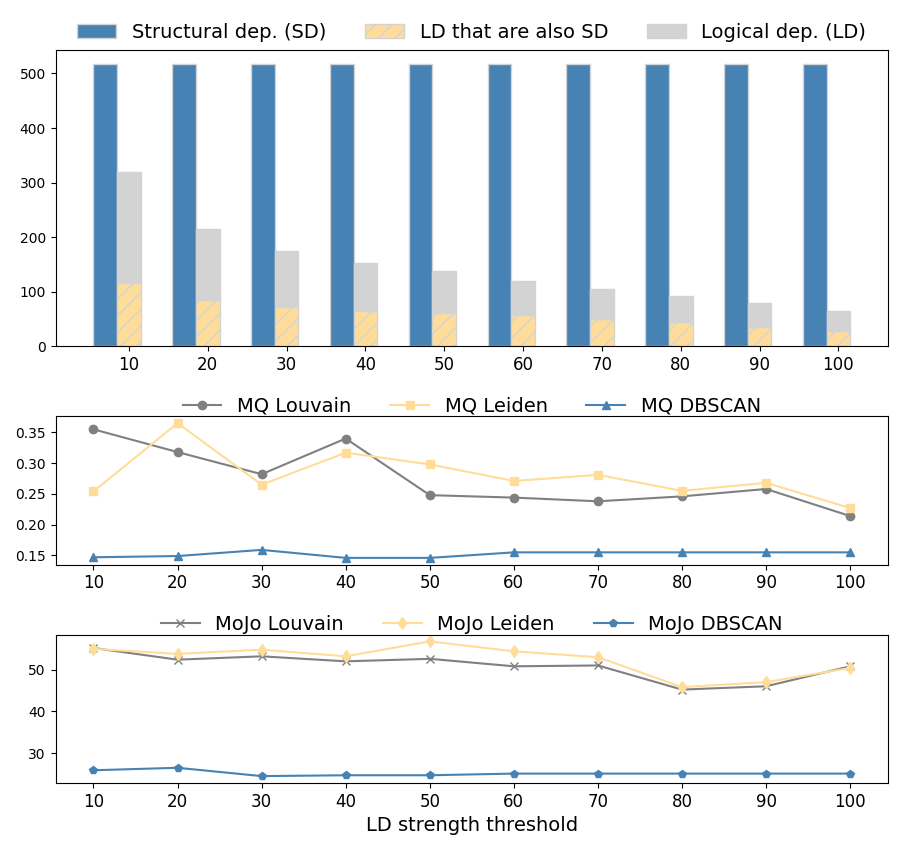
\includegraphics[width=\columnwidth]{ant_correlation.png}
\caption{Apache Ant: Overlap between structural and logical dependencies and its correlation with clustering metrics.}
\label{fig:ant_correlation}
\end{figure}

In our previous works, we studied how these two types of dependencies overlap \cite{b4}, \cite{DepSACI}. The reason behind those studies was to check how much new information we can get from using logical dependencies and how much is already present via structural dependencies.

Our overall findings were that with stricter filtering of logical dependencies, we obtain a higher percentage of overlap between the two dependencies, reaching at most 50\% of logical dependencies that are also structural dependencies.

So, we consider that the reason why SD+LD clustering solutions decline in performance with a higher strength threshold is that less and less new additional information is added to the system (logical dependencies that are not structural dependencies), causing the clustering solution to start resembling the performance of the SD-only solution. In Figure \ref{fig:ant_correlation}, we can see that LD(10) represents 61\% of the quantity of SD, while LD(100) is only at 12\%, with half of them being duplicated with SD.

\subsubsection{Apache Tomcat}

For Apache Tomcat (Table \ref{tab:clustering_results_tomcat}), the best results for SD+LD were obtained with strength thresholds between 10\% and 40\% across all algorithms. The Leiden algorithm achieved the best result for the MQ metric at a strength threshold of 40\%, while the best MoJoFM result was obtained at a threshold of 20\%, also with the Leiden algorithm. Compared with the SD-only results, the peak MQ values almost double the SD-only values. Like Apache Ant, the MQ values for all strength thresholds are higher than those for SD-only. While MoJoFM is not better for all thresholds, it still improves compared with the SD-only results.

The LD-only results show the highest MQ and MoJoFM values at LD(100) for the Louvain and Leiden algorithms. However, as with the Apache Ant results, coverage remains an issue. LD(100) covers only 16.62\% of the system, lower than the coverage from SD-only or SD+LD combinations. On the other hand, LD(10), which covers 61.33\% of the system, still has better clustering solutions compared to SD-only, based on both MQ and MoJoFM results.

We observe the same decline in results with a stricter strength threshold for SD+LD. As with the previous system, these results can again be connected to the percentage of LD that also overlaps with SD and the decreasing number of LD compared to SD once the strength threshold becomes stricter. As shown in Figure \ref{fig:catalina_correlation}, LD filtered with a 10\% strength threshold overlaps with SD by approximately 22\%, while at a 100\% strength threshold, the overlap increases to approximately 39\%.

\begin{figure}[t!]
\centering
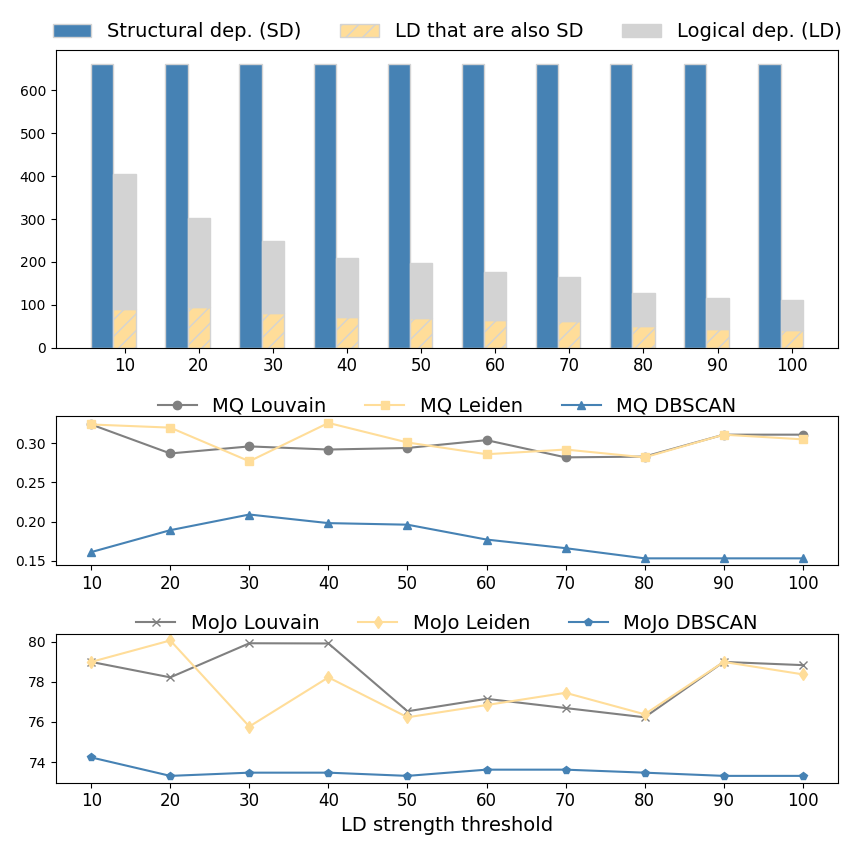
\includegraphics[width=\columnwidth]{catalina_correlation.png}
\caption{Apache Tomcat: Overlap between structural and logical dependencies and its correlation with clustering metrics.}
\label{fig:catalina_correlation}
\end{figure}

To ensure that the decline in performance for SD+LD with a stricter strength threshold is indeed caused by the fact that LD are significantly fewer than SD, and SD duplicates that part of them at higher thresholds, we added an additional experiment to our study. In this experiment, whose results can be found in Table \ref{tab:clustering_results_multiplication}, we increased the weights associated with LD(100) for Apache Tomcat to confirm that we are dealing with an LD quantity problem rather than a weight problem.

Therefore, in this experiment, we increased the weight assigned to each logical dependency filtered with a 100\% strength threshold from the Apache Tomcat system by values ranging from 1 to 5 and re-ran scenario III from Fig. \ref{fig:scenatrio}.


To maintain consistency, we used the same columns as in the other result tables (\ref{tab:clustering_results_ant}, \ref{tab:clustering_results_tomcat}, \ref{tab:clustering_results_hibernate}, \ref{tab:clustering_results_gson}), with the addition of two new columns:
\begin{itemize}
\item \textbf{Multiplication Factor:} The value by which each logical dependency weight is multiplied.
\item \textbf{Avg Weight:} The average weight assigned to each type of dependency used.
\end{itemize}

\begin{table}[htbp]
\centering
\caption{Impact of multiplication factors on clustering results for LD(100) in Apache Tomcat}
\label{tab:clustering_results_multiplication}
\resizebox{\textwidth}{!}{
\begin{tabular}{|l|c|c|ccc|ccc|ccc|}
\hline
\textbf{Multiplication} & \multicolumn{2}{c|}{\textbf{Avg. weight}} & \multicolumn{3}{c|}{\textbf{Louvain}} & \multicolumn{3}{c|}{\textbf{Leiden}} & \multicolumn{3}{c|}{\textbf{DBSCAN}} \\
\cline{4-12}
\textbf{Factor} & \textbf{SD} & \textbf{LD} & \textbf{Nr. of} & \textbf{MQ} & \textbf{MojoFM} & \textbf{Nr. of} & \textbf{MQ} & \textbf{MojoFM} & \textbf{Nr. of} & \textbf{MQ} & \textbf{MojoFM} \\
&  &  & \textbf{clusters} & &  & \textbf{clusters} & && \textbf{clusters} &  & \\
\hline
1 & 6.91  & 37.04  & 31 & 0.311 & 78.83 & 31 & 0.305 & 78.37 & 43 & 0.153 & 73.31 \\
2 & 6.91  & 74.08  & 33 & 0.295 & 73.57 & 30 & 0.301 & 72.33 & 43 & 0.153 & 73.31 \\
3 & 6.91  & 111.12 & 34 & 0.313 & 74.19 & 33 & 0.309 & 72.80 & 43 & 0.153 & 73.31 \\
4 & 6.91  & 148.16 & 34 & 0.312 & 73.88 & 33 & 0.312 & 72.49 & 43 & 0.153 & 73.31 \\
5 & 6.91  & 185.20 & 34 & 0.306 & 73.88 & 33 & 0.308 & 72.18 & 43 & 0.153 & 73.31 \\
\hline
\end{tabular}

}
\end{table}


In Table \ref{tab:systems_weights}, which presents the average weights associated with the dependencies across all systems, we can see that for Tomcat, the average weight for LD(10) is already almost double the SD average weight. For LD(100), the average weight is approximately five times higher than that of SD.

Based on the metric values obtained for multiplication factors of 2 to 5, we can see that after increasing the weights assigned to LD, the metric values improve only slightly, with changes recorded at the second decimal: a 0.02 improvement for Louvain and 0.07 for Leiden. The results for DBSCAN remain unchanged due to the fixed values of MinPts and Eps and the already high LD weights for LD(100).

We can conclude from the experiment with weights that the issue is the quantity of dependencies. SD outnumbers LD, making LD information less impactful on the clustering solution.


\subsubsection{Hibernate ORM}

Hibernate ORM is the second largest system after Apache Tomcat regarding the number of commits analyzed, with 16,609 commits considered for LD extraction. Additionally, it is the largest in terms of system size, with 4,414 entities (Table \ref{tab:project_info}).

Based on the results from Table \ref{tab:clustering_results_hibernate}, the SD+LD combination with a strength threshold of 40 performs best for this system. Louvain achieves the best MQ metric at this threshold, while Leiden achieves the best MoJoFM metric.

LD-only produced the best MQ values at 100\% strength and the best MoJoFM values at 70\% strength for both Louvain and Leiden. Compared to the previous systems, where both best values were recorded at the same strength threshold, Hibernate shows an earlier peak for MoJoFM. The system coverage is likely a factor contributing to this. Hibernate  LD[100] covers only 8.07\% of the system, the lowest percentage among all systems studied. This low percentage can be linked to the number of commits compared to the number of entities. For Apache Tomcat, there were 22,698 commits and 662 entities, while for Hibernate, there were 16,609 commits and 4,414 entities. This indicates that not all entities had a chance to be updated in the version control system.

This observation is also reflected in Table \ref{tab:systems_weights}, where Hibernate has the lowest average weights for LD compared to SD across all systems. In other systems, LD(10) starts with almost double the average weight compared to SD, while Hibernate's LD(10) average weight is less than half of the SD average weight.

\begin{figure}[t!]
  \centering
  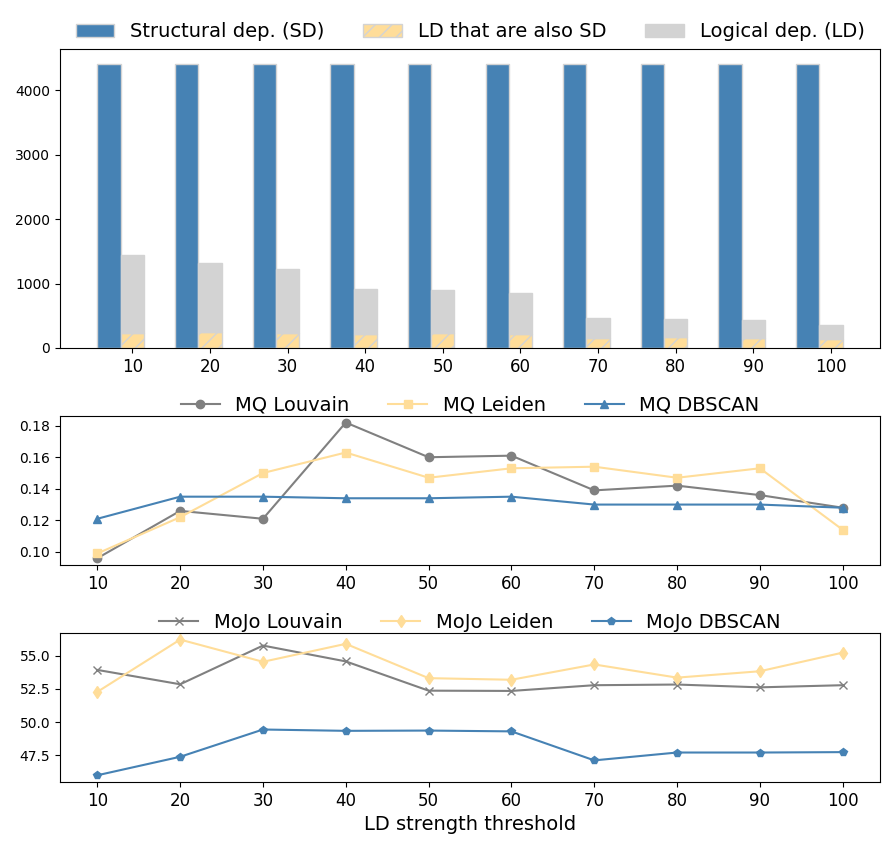
\includegraphics[width=\columnwidth]{hibernate_correlation.png}
  \caption{Hibernate ORM: Overlap between structural and logical dependencies and its correlation with clustering metrics.}
  \label{fig:hibernate_correlation}
\end{figure}

Hibernate has the lowest overlap percentage between LD and SD, as shown in Figure \ref{fig:hibernate_correlation}. Similar to the other systems, the performance for MQ and MoJoFM decreases for SD+LD as the strength threshold becomes stricter.

The results for Hibernate highlight the challenge of achieving better clustering in larger systems with fewer commits relative to their size.


\subsubsection{Google Gson}


\begin{figure}[t!]
  \centering
  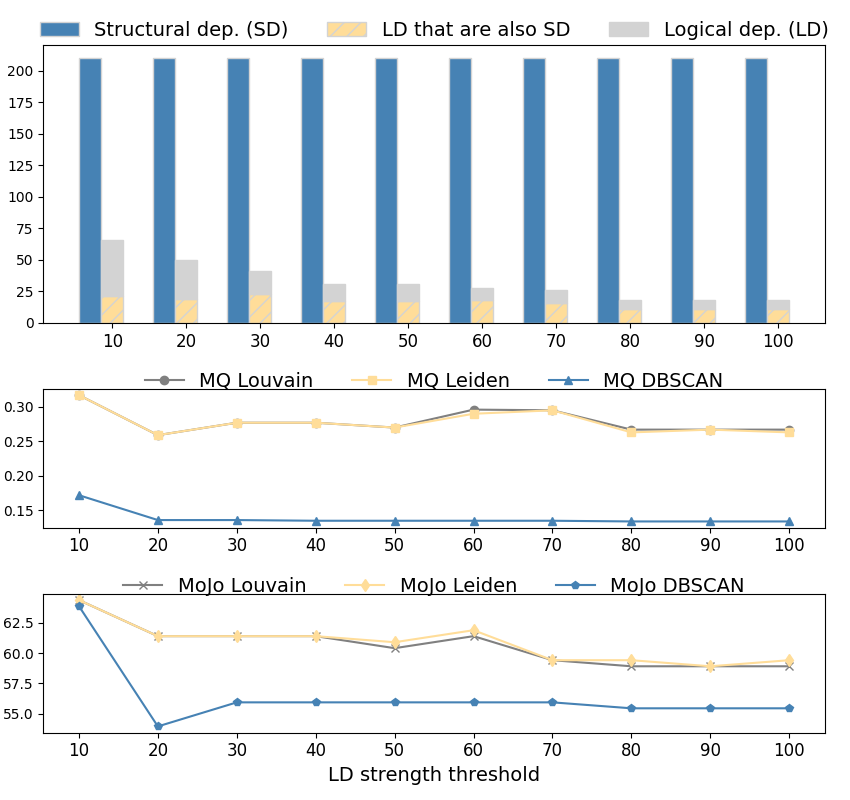
\includegraphics[width=\columnwidth]{gson_correlation.png}
  \caption{Google Gson: Overlap between structural and logical dependencies and its correlation with clustering metrics.}
  \label{fig:gson_correlation}
\end{figure}

Gson has the smallest number of commits analyzed, with 1,772 commits considered for LD extraction, and it is also the smallest in terms of system size, with 210 entities involved in clustering (Table \ref{tab:project_info}).

Based on the results from Table \ref{tab:clustering_results_gson}, the SD+LD combination with a strength threshold of 10 achieved the best results for both MQ and MoJoFM. Like Apache Ant and Tomcat, all SD+LD combinations achieve better MQ values than SD-only.

LD-only produced the best results for MQ at 40\% strength for both Louvain and Leiden, and the best MoJoFM value was also observed at the same threshold for both algorithms. It is the only system where the best MQ result for LD-only occurs at a lower strength threshold than 100\%. This is due to the very low number of entities remaining in the system at 100\% (only 18 out of 210).

In this particular system, it is more visible that the Leiden clustering algorithm does not improve the Louvain algorithm in some scenarios. This observation is based on the fact that the values obtained for both MQ and MoJoFM metrics are the same in most cases for the Gson system for both algorithms.

It can also be observed that Gson has identical metric values for MQ and MoJoFM across multiple strength thresholds. Again, the small number of commits and the size of the system contribute to the stability of these metrics.

Gson also has relatively high overlap rates between LD and SD compared to the other systems, as shown in Figure \ref{fig:gson_correlation}. Despite the constant values, the trend of decreasing performance for SD+LD with stricter strength filtering for LD is also present in Gson.

The results for this system highlight the difficulty of achieving better clustering solutions using logical dependencies in smaller systems with fewer commits. However, even for a small system like Gson, an improvement is still visible when using logical dependencies.


\subsection{Discussion on Ant clustering}
\label{discussion_ant}

Based on the results from Table \ref{tab:clustering-results2}, we can observe that the combined approach of structural dependencies and logical dependencies gives the highest Modularity Quality (MQ) metric of 0.227 with a strength threshold of 30\%, which is an improvement over the 0.08 MQ metric obtained when considering only structural dependencies.

Beyond the positive result indicated by the MQ metric, we searched for further validation by human software engineering expert opinion. After thoroughly studying and understanding the analyzed system source code and documentation, we evaluated the remodularization proposals resulting from the two clustering solutions.

The two clustering solutions compared are the clustering solution obtained only from structural dependencies, in comparison to the clustering solution obtained from using both structural and logical dependencies, filtered with a threshold of 30\% for strength.

The clustering solution relying solely on structural dependencies consists of 12 clusters, while the solution using both structural and logical dependencies consists of 15 clusters. Both solutions involve the same number of entities (517). The entities listed below are placed in different clusters:

\begin{itemize}
    \item taskdefs.Available\$FileDir
    \item taskdefs.Concat and its inner classes taskdefs.Concat\$1, taskdefs.Concat\$MultiReader, taskdefs.Concat\$ TextElement
    \item taskdefs.Javadoc\$AccessType
    \item util.WeakishReference and its inner class util.WeakishReference\$HardReference
    \item taskdefs.Replace and its inner classes taskdefs.Replace\$ NestedString, taskdefs.Replace\$Replacefilter
\end{itemize}

The migration of entities between clusters is illustrated in Figure \ref{fig:clustersmigration}. Given that the inner classes are shifted from one cluster to another in the same way as the outer class, we omitted the inner classes from the diagram.

As the cluster number itself is not significant and may vary across different script runs (labels might vary), we will refer to each individual cluster resulting from structural dependencies as \textit{Cluster A} and to the ones resulting from both logical and structural dependencies as \textit{Cluster B}.

\begin{figure}
\centering
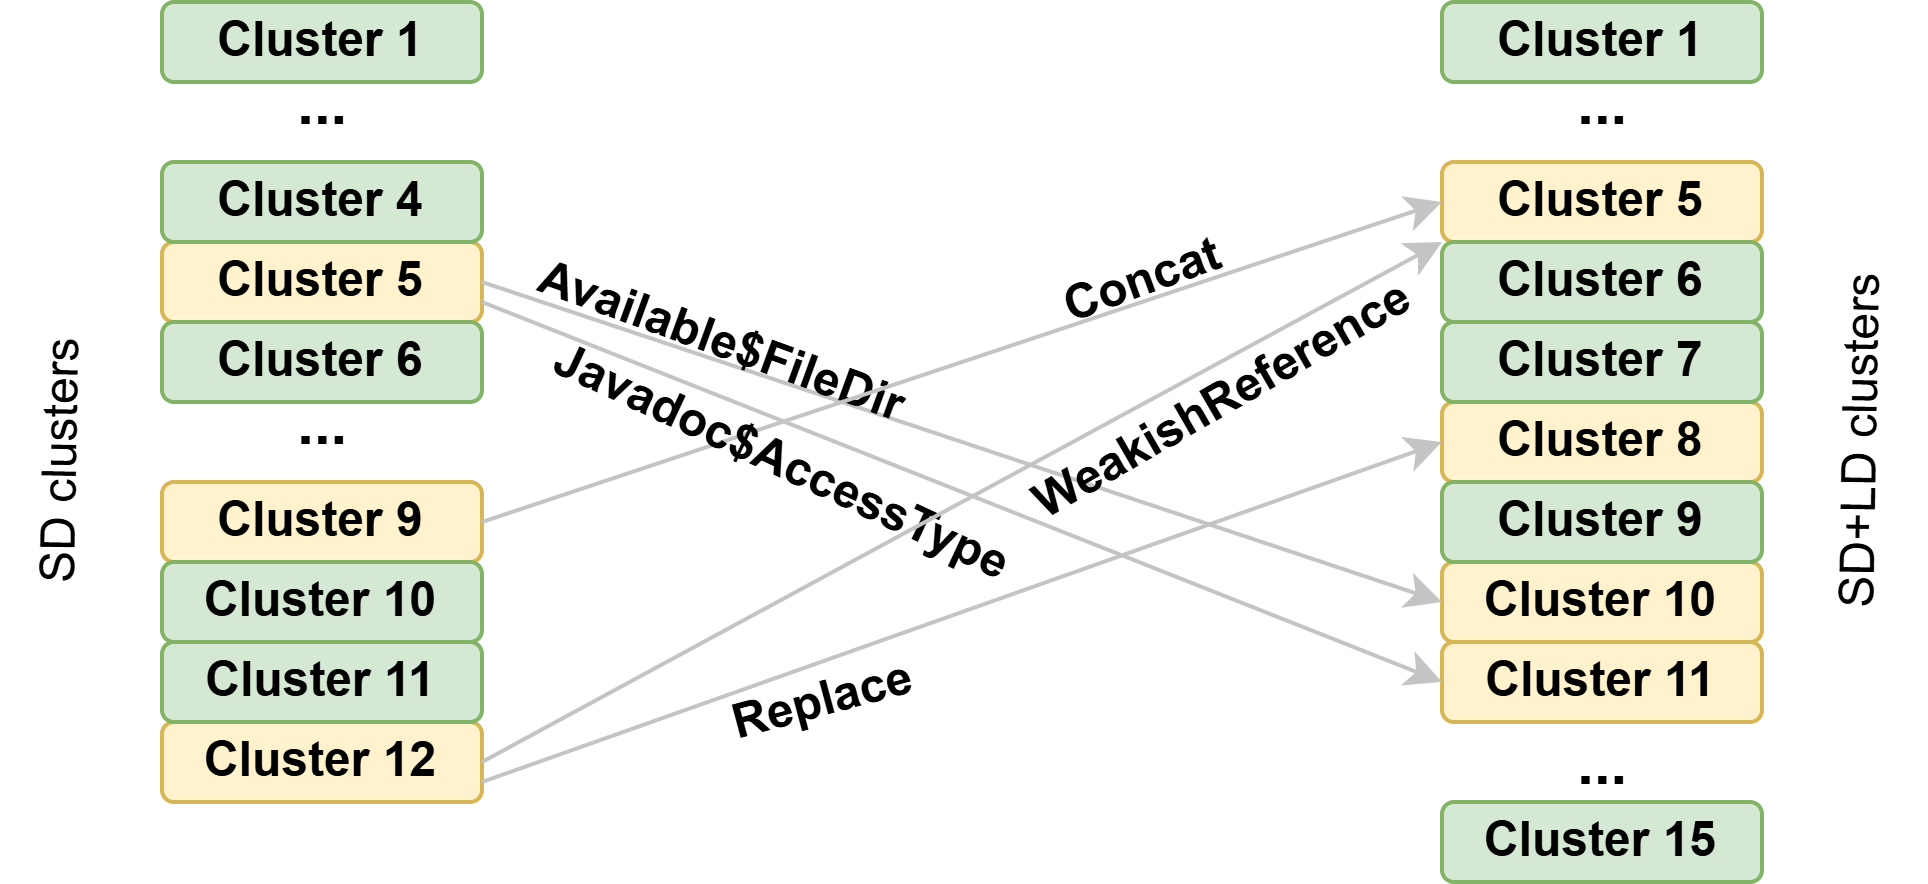
\includegraphics[width=\columnwidth]{clusters.png}
\caption{Migration of entities between clusters}
\label{fig:clustersmigration}
\centering
\end{figure}

\subsubsection{taskdefs.Concat and its inner classes}

To have a better overview of how and why entities are transferred between clusters, we depicted Concat's logical and structural connections in Figure \ref{fig:dep_concat}. Additionally, Figure \ref{fig:clusterAconcat} illustrates connections within Cluster A, while Figure \ref{fig:clusterBconcat} does the same for Cluster B.

In Cluster A, the Concat class and its inner classes (Concat\$1, Concat\$MultiReader, Concat\$TextElement) are placed together with conditions like Available, And, Or, IsTrue, Equals, IsReference, Contains.

On the other hand, in Cluster B, they are placed with classes associated with file manipulation and archive operations such as Ear, Jar, War, and Zip, as well as utility classes for file handling like FileUtils and JavaEnvUtils, and entities for zip file processing (ZipEntry, ZipFile). This placement is due to the logical dependencies that Concat class has with FileUtils and FileSet in the versioning system.

To assess whether the placement of Concat in Cluster B is better than in Cluster A, we referred to the official Ant documentation. According to the documentation: "This class contains the 'concat' task, used to concatenate a series of files into a single stream" \cite{ant_concat}. Therefore, judging by its usage and purpose according to the documentation, positioning the Concat class along with its inner classes in Cluster B is more suitable than in Cluster A.


\begin{figure}
\centering
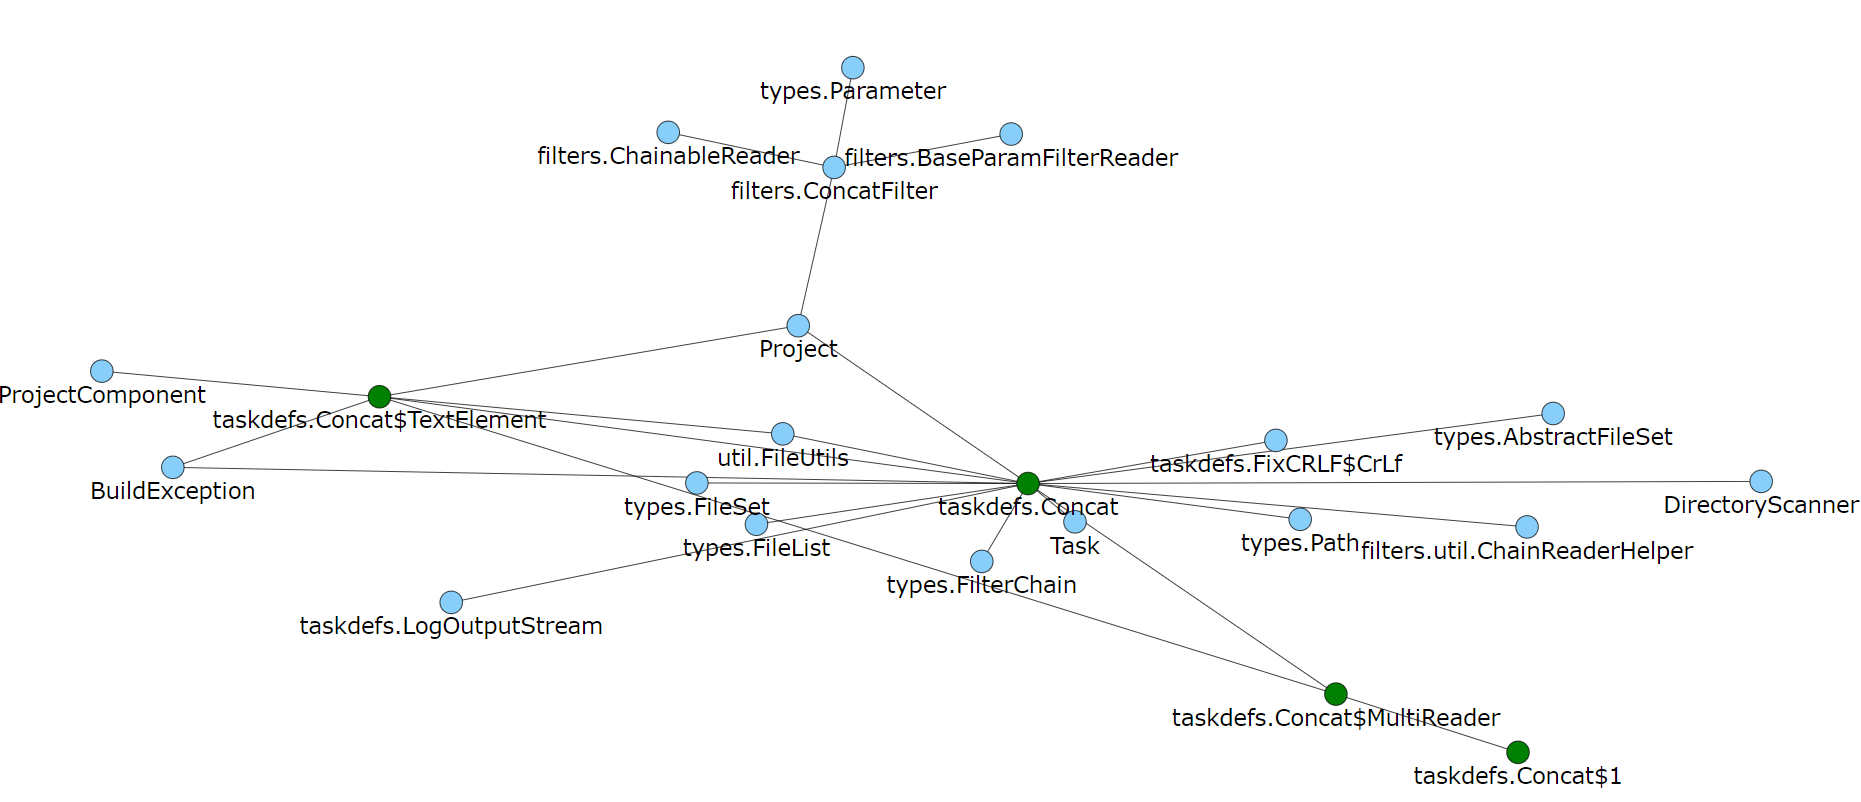
\includegraphics[width=\columnwidth]{dep_concat.png}
\caption{Dependencies (LD and SD) of Concat class}
\label{fig:dep_concat}
\centering
\end{figure}


\begin{figure}
\centering
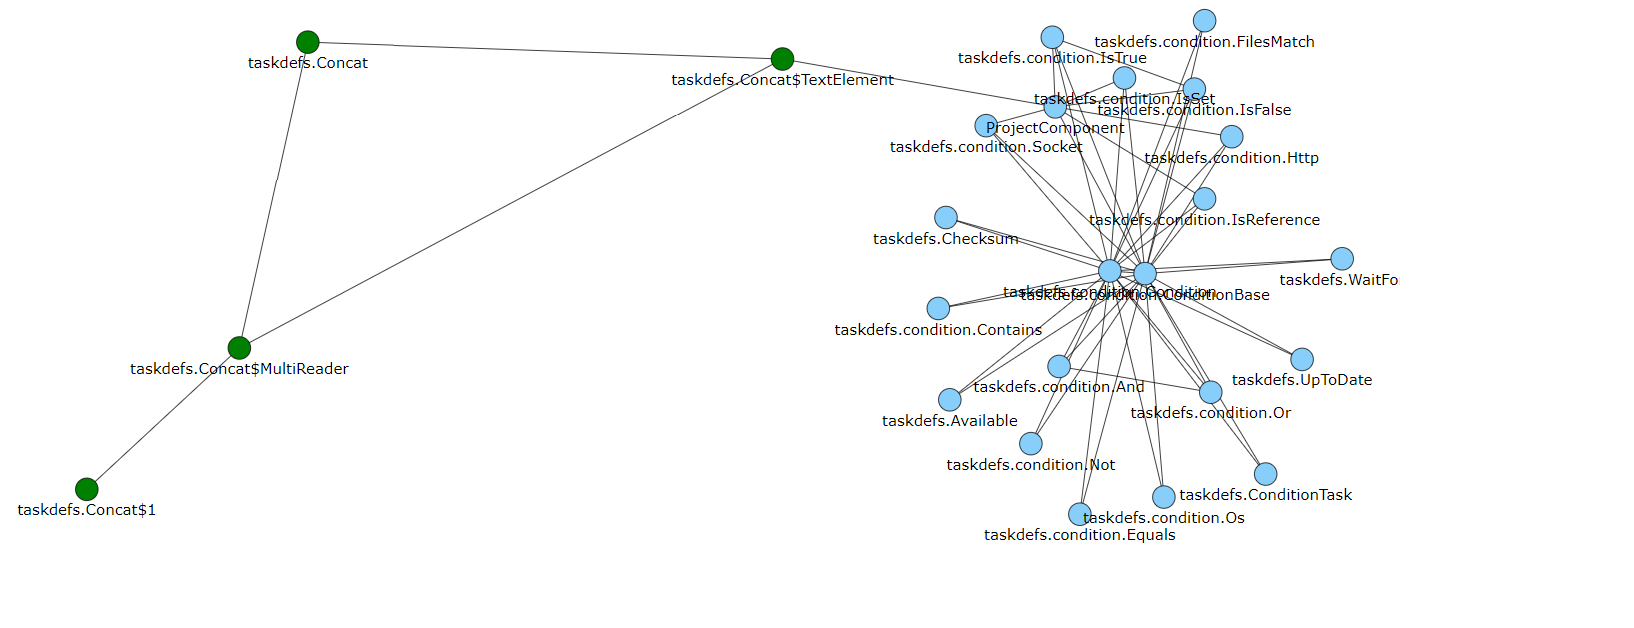
\includegraphics[width=\columnwidth]{cluster_concatSD.PNG}
\caption{Placement of Concat in ClusterA (SD); cluster size: 25}
\label{fig:clusterAconcat}
\centering
\end{figure}


\begin{figure}
\centering
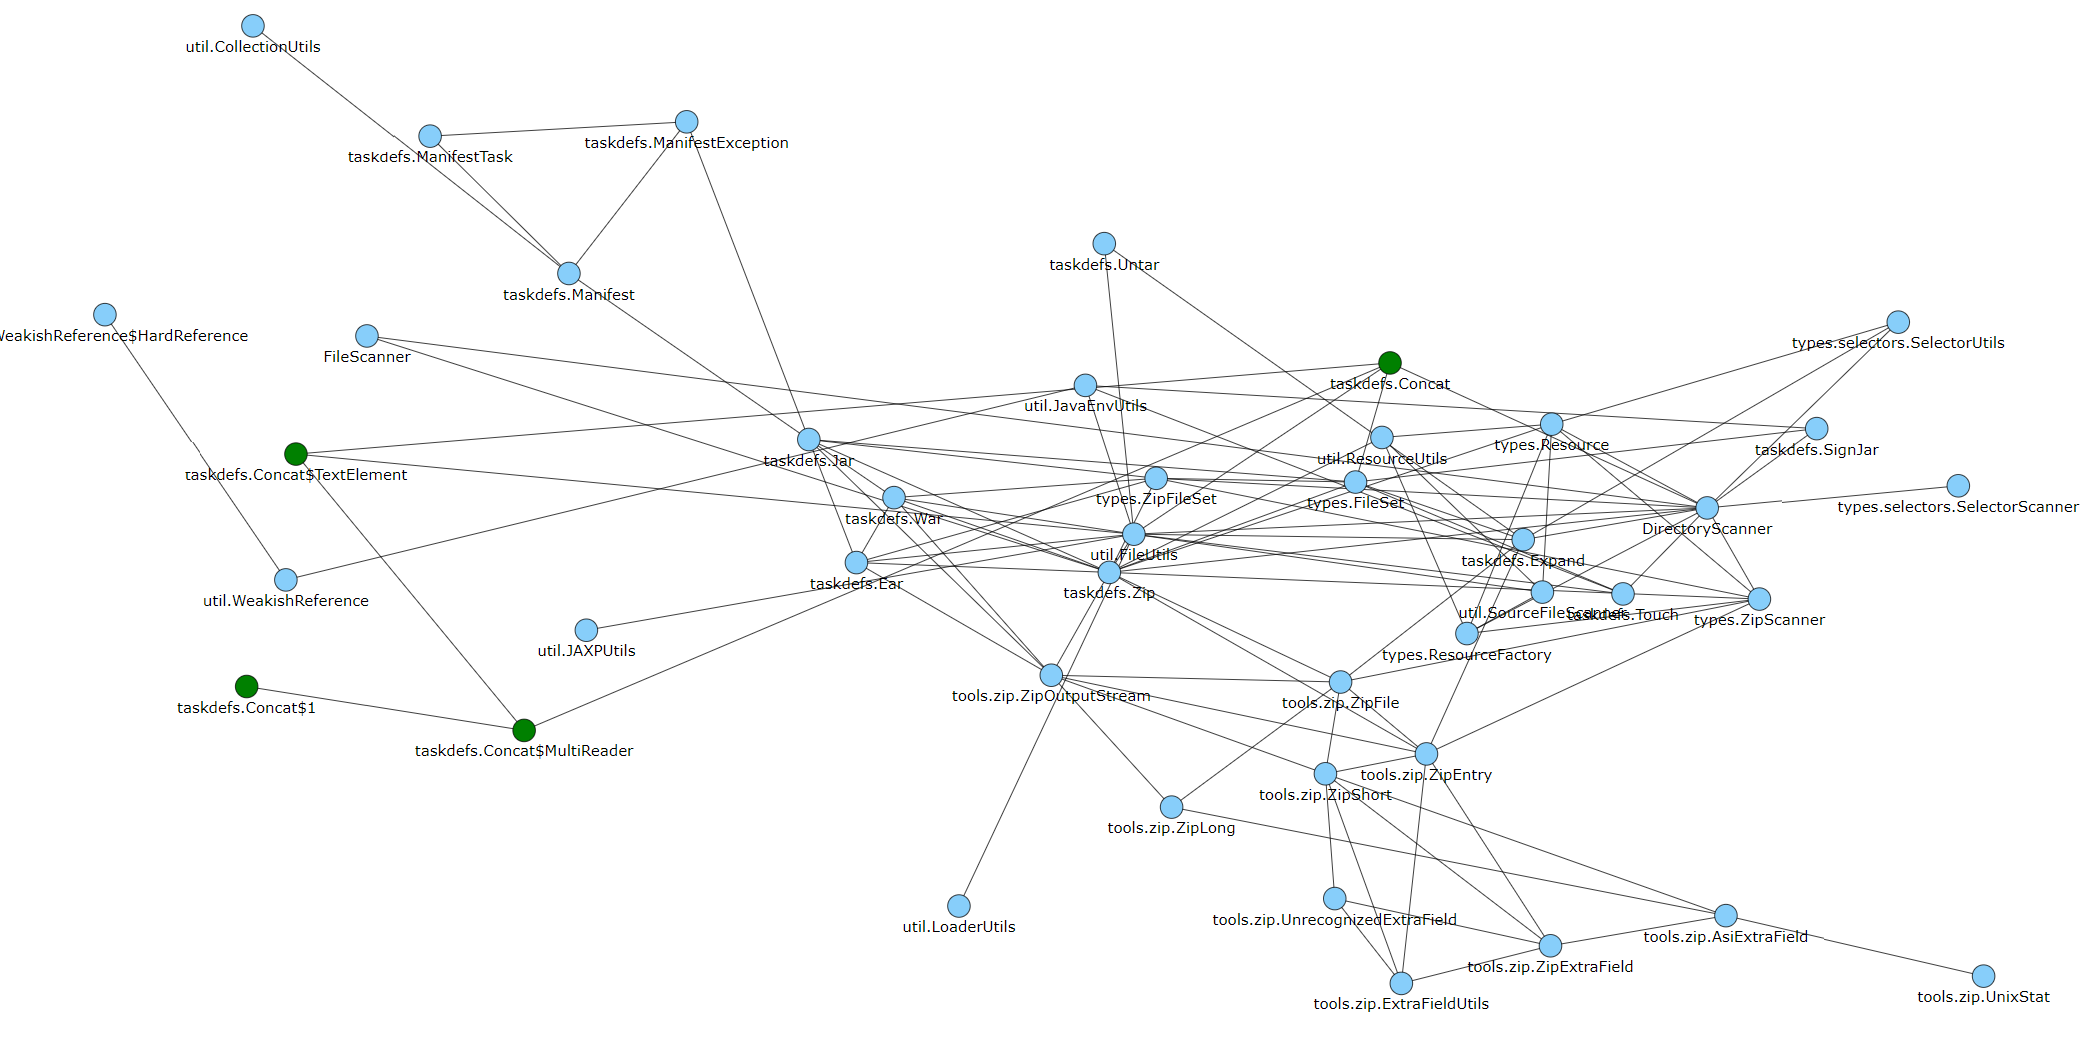
\includegraphics[width=\columnwidth]{cluster_concatSDLD.PNG}
\caption{Placement of Concat in ClusterB (SD and LD); cluster size: 52}
\label{fig:clusterBconcat}
\centering
\end{figure}

\subsubsection{taskdefs.Available\$FileDir}

In Cluster A the entity 'taskdefs.Available\$FileDir' is in the same cluster with entities that are related to the build process (ProjectHelper, TaskAdapter, ComponentHelper), but not with entities that have any relation to condition checks or file existence evaluations or with its outer class. 

Cluster B contains entities that are related to condition checking (And, Contains, Equals, Or, UpToDate), and also with the outer class of 'taskdefs.Available\$FileDir',  'taskdefs.Available'. The movement of entities from Cluster A to Cluster B was influenced by the logical dependencies between 'taskdefs.Available' and 'taskdefs.Available\$FileDir'.

The documentation description for 'taskdefs.Available' states: "Will set the given property if the requested resource is available at runtime. This task may also be used as a condition by the condition task."\cite{ant_concat}.
This reinforces its placement in Cluster B, which is centered around task definitions and conditions related to build processes.



\subsubsection{ taskdefs.Replace and its inner classes}

\begin{figure}
\centering
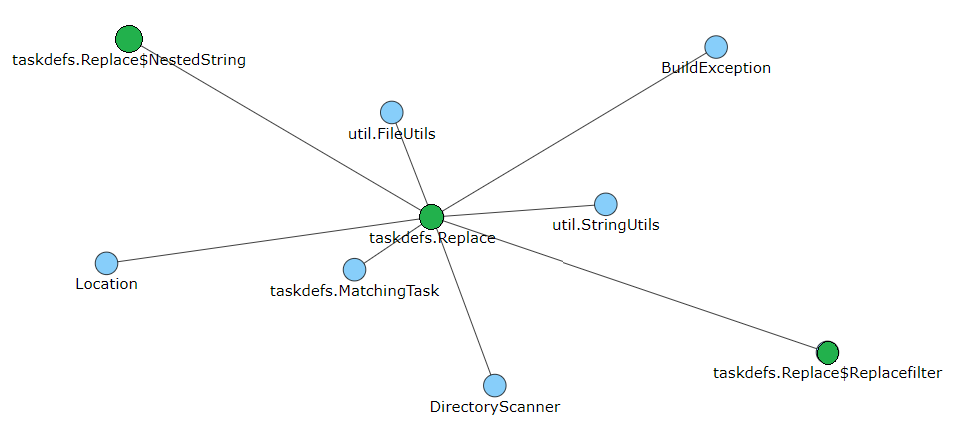
\includegraphics[width=\columnwidth]{dep_replace.png}
\caption{Ant dependencies (LD and SD) of Replace and its inner classes}
\label{fig:dep_replace}
\centering
\end{figure}

\begin{figure}
\centering
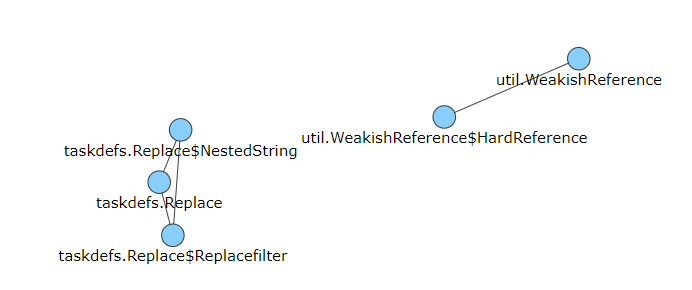
\includegraphics[width=\columnwidth]{cluster_replaceSD.PNG}
\caption{Placement of Replace in ClusterA (SD); cluster size: 5}
\label{fig:clusterAreplace}
\centering
\end{figure}


\begin{figure}
\centering
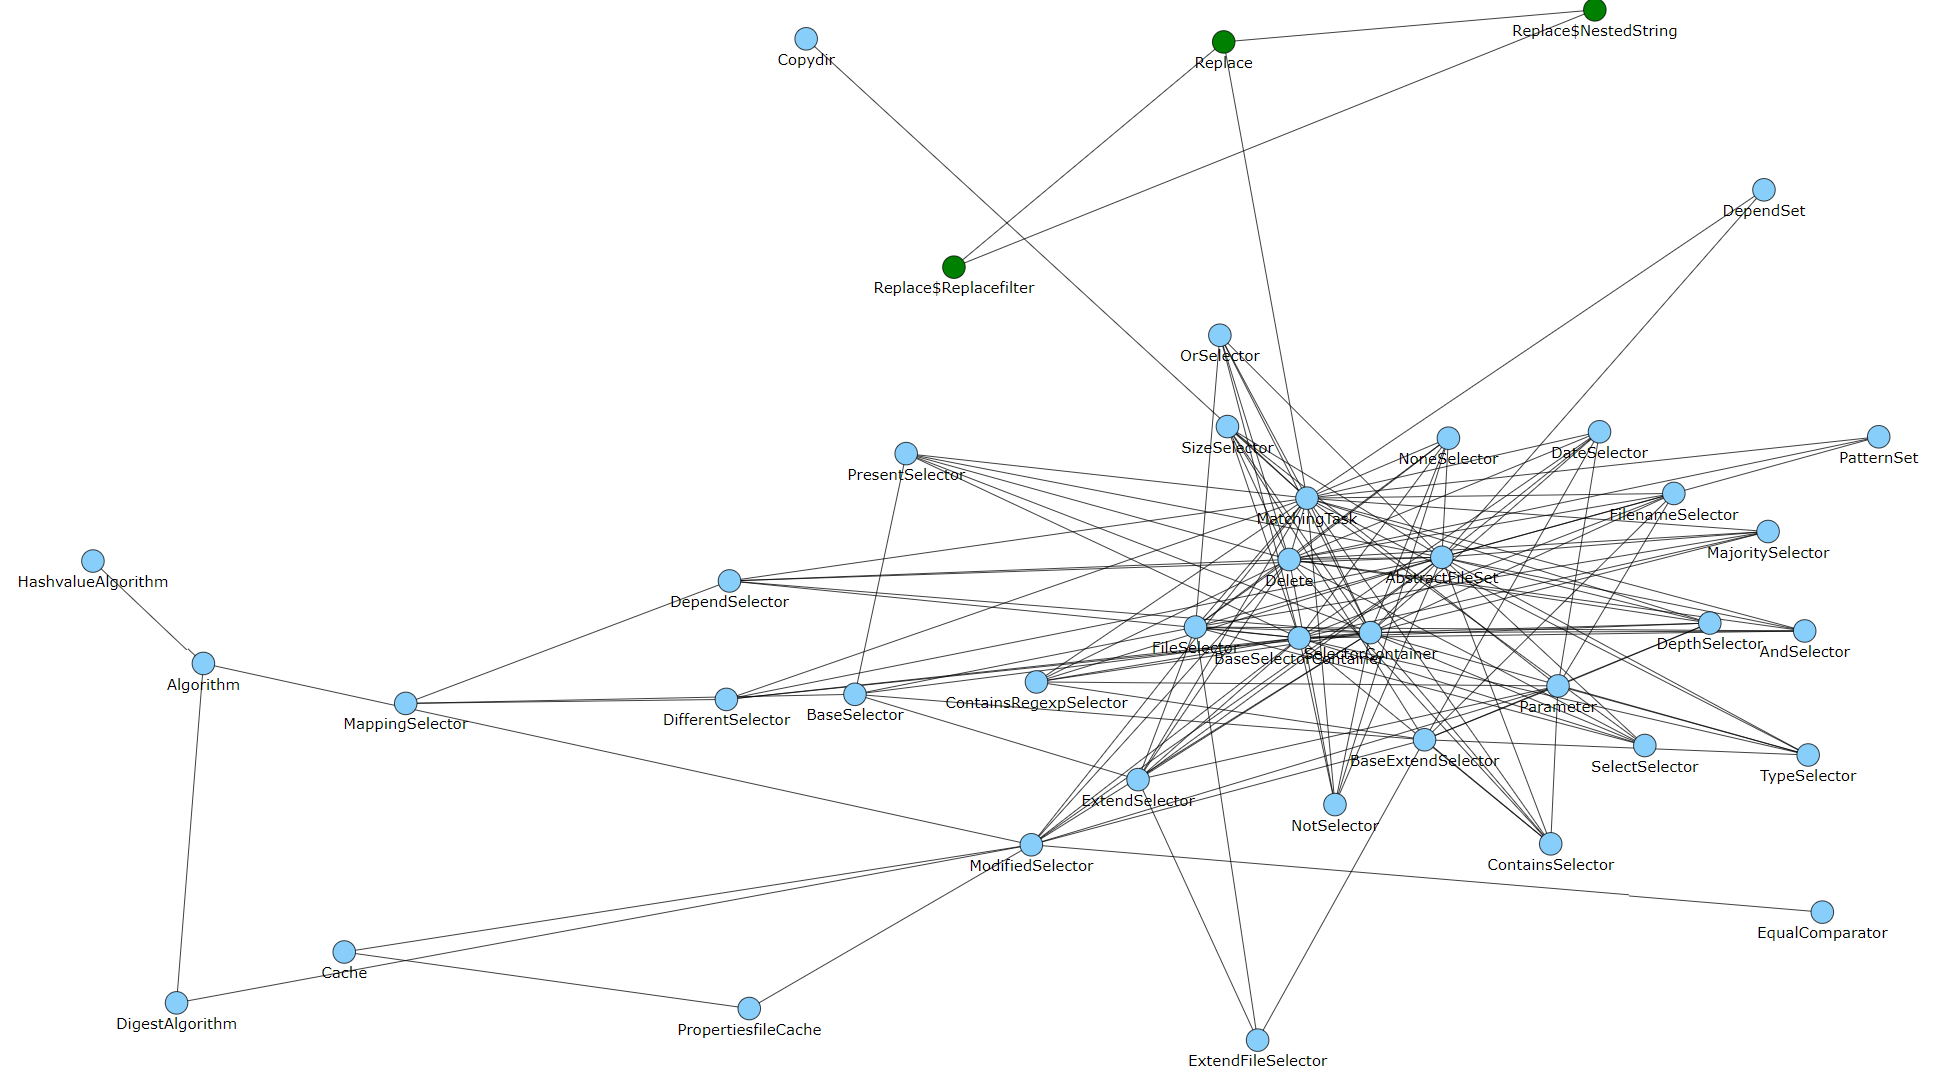
\includegraphics[width=\columnwidth]{cluster_replaceSDLD.PNG}
\caption{Placement of Replace in ClusterB (SD and LD); cluster size: 42}
\label{fig:clusterBreplace}
\centering
\end{figure}


We depicted the logical and structural connections of Replace in Figure \ref{fig:dep_replace}. Figure \ref{fig:clusterAreplace} illustrates connections within Cluster A, while Figure \ref{fig:clusterBreplace} does the same for Cluster B.

Replace and its inner classes are placed in Cluster B with entities with which they share common functionality and purpose, such as Copydir, Delete, DependSet, or MatchingTask. These entities are involved in similar tasks and operations. On the other hand, the placement in Cluster A, with WeakishReference and its inner class doesn't seem good, as these entities are completly unrelated.  

The movement of entities from Cluster A to Cluster B was influenced by the strong logical dependency between 'taskdefs.Replace' and 'taskdefs.MatchingTask'.

The cluster from figure \ref{fig:clusterAreplace} is the 12th cluster from the clustering solution based on structural dependencies. This particular cluster is essentially comprised of two unrelated entities: Replace and WeakishReference. Due to their logical dependencies, both entities are grouped within larger clusters that share similar functionalities in the SD and LD solution \cite{icstcc-2024}.


\subsection{Research questions and findings}

In this section, we will answer our research questions based on the results of our experiments. 

\textit{ \textbf{RQ1:} Does using structural dependencies (SD) combined with logical dependencies (LD) improve software clustering results compared to traditional approaches using only structural dependencies (SD)?} 

Based on the results from all four systems analyzed, the combination of SD and LD performed better than SD-only according to the MQ and MoJoFM metrics, confirming that using SD+LD improves software clustering results. Across different strength thresholds, SD+LD achieved higher MQ and MoJoFM values for all clustering algorithms, indicating better modularization. 
The filtering thresholds applied to logical dependencies influence the effectiveness of combining SD and LD. Lower strength thresholds (10\% to 40\%) resulted in better MQ and MoJoFM values across all clustering algorithms compared with higher thresholds.

At higher strength thresholds, the MQ and MoJoFM results decline. This decline occurs because stricter strength thresholds significantly reduce the amount of logical dependencies. This reduction leads to fewer new relationships introduced into the clustering process. Our previous research on the overlap between SD and LD showed that higher strength thresholds correlate with increased overlap between the two dependencies. This overlap indicates that at higher strength thresholds, not much new information is added to the system besides what is already introduced by structural dependencies, reducing the impact of logical dependencies on clustering results.

However, when considering a lower strength threshold, the relationship between the system size and the number of commits in the version history becomes an important factor.

In the case of Hibernate, a stricter strength threshold was needed to achieve the best metric values compared to other systems. Although the metrics obtained at a 10\% strength threshold for LD are better than SD-only, the system reached peak metric values at 40\% threshold across all algorithms.

With 16,609 commits and 4,414 entities, Hibernate has a significantly lower average number of commits per entity than Ant (14,917 commits and 517 entities) or Tomcat (22,698 commits and 662 entities). This lower ratio means that each entity in Hibernate is, on average, involved in fewer commits. As a result, the co-change data extracted for logical dependencies are sparser and contain more noise at lower strength thresholds.

A stricter strength threshold (e.g., 40\%) filters out these weaker logical dependencies.

In contrast, systems like Ant and Tomcat, with higher ratios of commits to entities, obtain better results with logical dependencies at a 10\% strength threshold because entities participate in more commits on average.

In conclusion, with an appropriate threshold, combining SD with LD leads to better clustering results than using SD alone.


\textit{\textbf{RQ2:} Can using only logical dependencies (LD) produce good software clustering results?} 

Using LD-only produced good clustering results, especially at higher strength thresholds. LD(100) produced the highest MQ and MoJoFM values for most systems compared with SD-only and SD+LD. However, the coverage of LD-only is significantly lower at these higher thresholds. For all systems, after filtering with 100\% strength threshold, the system coverage of the remaining logical dependencies is less than 17\% of the total known dependencies in the system.

Thus, while LD(100) provides the highest metric results compared to SD+LD and SD-only, it represents only a small subset of the system's dependencies.

On the other hand, LD(10) has, in most of the cases, better metric results than those for SD-only and SD+LD with better system coverage. Apache Ant and Tomcat LD(10) cover more than 60\% of the system, while for Hibernate and Gson, the coverage is slightly above 30\%. 

Therefore, LD(10) can be an alternative to SD-only or SD+LD, especially if structural dependencies are not available.

It is also important to consider that LD-only performance at higher strength thresholds depends on the system's characteristics, such as the number of commits and entities. For Gson project, the performance at a 100\% strength threshold is not as good as for the other systems, reaching its peak at a 40\% threshold. This is due to the low number of entities remaining at higher thresholds, with only 18 entities at the 80\% to 100\% strength thresholds, and the relatively small number of commits considered.

In summary, while LD-only can produce good clustering results, especially at higher strength thresholds, its limited coverage reduces its usability, as the clustering is intended for the entire system, not just a small subset. LD-only offers a good alternative to SD-only at lower strength thresholds, providing acceptable coverage.

\textit{ \textbf{RQ3:} How do different filtering settings for logical dependencies (LD) impact clustering results, and which filtering settings provide the best performance?}

The impact of different filtering settings on clustering performance was observed across all systems. For LD-only clustering, lower strength thresholds like 10\% provided good system coverage but had lower MQ and MoJoFM values compared to higher thresholds like 100\%, where the best metric results were often achieved. However, at these higher thresholds, the system coverage was significantly reduced.

The best performance was generally observed with strength thresholds between 10\% and 40\% for the combination of SD and LD (SD+LD). At these thresholds, the clustering solutions achieved higher MQ and MoJoFM values than SD alone.

It is important to select the optimal filtering threshold. Logical dependencies filtered with lower strength thresholds include more relationships, introducing more knowledge that could improve clustering results. However, a too-low threshold may sometimes introduce noise, especially in systems with a low commits-to-entities ratio. On the other hand, higher thresholds significantly reduce noise but can exclude valuable dependencies and decrease coverage.

The optimal filtering threshold may vary depending on system characteristics ( number of commits, size of the system), so it is important to consider these factors when filtering logical dependencies.




\newpage
\addcontentsline{toc}{section}{References}
\nocite{*}
\bibliographystyle{unsrt}
\bibliography{references}

\end{document}
